\documentclass[bachelor,english]{infothesis}
% possible types: bachelor, master, zula (seminar, practical)
% Für Seminararbeiten und Praktikumsberichte die Vorlage my-seminar-praktikum.tex verwenden!
% possible languages: english, german

\usepackage[utf8]{inputenc}
\usepackage[T1]{fontenc}
\usepackage{lmodern}
\usepackage{svg}
\usepackage{pythonhighlight}
\usepackage{longtable}

\graphicspath{{figures/}}


%%%%%%%%%%%%%%%%%%%%%%%%%%%%%%%%%%%%%%%%%%%%%%%%%%%%%%%%%%%%%%%%%%%%%%%%%%
%%%%%%%%%%%%% Bitte nur ab hier Änderungen vornehmen %%%%%%%%%%%%%%%%%%%%%

\title{Reinforcement Learning for Control of Flying Drones} 

\author{Johannes M. Tölle} 

\submissiondate{06. 09. 2023} 

\supervisors{% Geben Sie die Namen aller Betreuer ab, getrennt durch das Makro '\and'
%Prof.\ Dr.\ Günther Waxenegger-Wilfing \and
%Prof.\ Dr-Ing.\ Sergio Montenegro \and
Prof.\ Dr.\ Carlo D'Eramo
} 

\renewcommand{\contentsname}{Table of Contents}
\renewcommand{\listfigurename}{List of Figures}
\renewcommand{\listtablename}{List of Tables}
%\renewcommand{\listalgorithmname}{List of Algorithms}

\newenvironment{declaration}
{\chapter*{Declaration}}
{}


\begin{document}
%vspace*{12cm}\\
\topskip0pt
\vspace*{\fill}
\begin{center}
	\Huge
	\emph{"Success is walking from failure to failure with no loss of enthusiasm.\\
	\qquad \qquad \qquad- Winston Churchill"}
\end{center}
\vspace*{\fill}
\thispagestyle{empty}
\newpage
\pagenumbering{roman}
	
\begin{declaration}
	I certify that I have authored this thesis, including all attached materials,
	constantly and without the use of any other aids than those specified.\\
	All passages taken literally or analogously from published or unpublished works
	are clearly identified as such in each individual case, stating the source.\\
	The work has not yet been submitted in the same or a similar form as a thesis.\\
	I am aware that violations of this declaration and deliberate deception may lead to
	a grade of 5.0.\\
	\vspace*{12cm}\\
	Würzburg, \today 
	\hspace*{\fill}\begin{tabular}{@{}l@{}}\hline
	\makebox[4cm]{Johannes M. Tölle}
	\end{tabular}
\end{declaration}

\tableofcontents
\listoffigures
\listoftables
\listofalgorithms

\begin{abstract}
	\addcontentsline{toc}{chapter}{Abstract}
	The control of drones, also known as unmanned aerial vehicles (UAV), 
	is a difficult task which is of great interest to modern research.
	Modern UAVs are in need of reliable, precise, and robust flight control in order to
	be able to operate in a wide range of environments. Especially in harsh environments,
	the performance of classic controllers is far from optimal.
	Reinforcement Learning is known for its ability to create intelligent, robust
	controllers that can operate in harsh environments. In order to achieve this, the learning process
	should not get stuck in local optima and well generalize the complex problem. The use 
	of curricula in Reinforcement Learning has shown to improve the learning process, because
	of countering the exploration-exploitation trade-off.
	This work proposes a simple intelligent flight control based on 
	different intelligent controllers that were trained for
	a couple of UAV flight problems. Furthermore, it emphasizes the importance of 
	well-designed curricula on random goal modes based on a linear curricula automation approach (LCL).
	In addition, it aims at providing a general overview of intelligent flight
	control and promises ideas for future work in this designated area of research that can further improve 
	the performance.
\end{abstract}




%\thesistableofcontents




%%%%%%%%%%%%%%%%%%%%%%%%%%%%%%%%%%%%%%%%%%%%%%%%%%%%%%%%%%%%%%%%%%%%%%%%%%%%%%%%
\setcounter{page}{1}
\pagenumbering{arabic}
\chapter{Introduction}
	In the last decade, an increase of popularity in the area of automated flight
control could be observed. While a wide range of companies sell classic
drones like Quadrocopter, these are mostly remotely piloted and used for
hobby purposes.
However, automated flight control can simplify many jobs and in total a
lot of work can be accomplished more efficiently.
In addition, autonomous UAVs can even be used in a wider range of application,
because a pilot is not needed.
Therefore, autonomous UAVs can operate in misanthropic, harsh environments.
Also, there are environments that hinder direct piloting.\\
For example, in tunnel-like environments like sewers flight control has to be accurately
executed, because the tunnels can have small diameters. In addition,
the environment is not directly viewable and piloting relies on video material
that might be delayed and requires a given infrastructure. \\
Also, modern agriculture starts using drones for autonomous seed dropping or
as a low-cost remote sensing system. The variety of possible applications 
for autonomous UAVs is immense and is increasing til today.
As a consequence, also an increase of research could be observed - specializing 
on different aspects on this complex task.
One of these aspects is the accuracy of the drone: the ability to approach 
a defined waypoint and keep this position as accurately as possible if desired.
Also increasing the velocity of waypoint approaching has been researched.
For many tasks it is important to keep a steady flight in order to
use payloads like cameras effectively.
Therefore, high rotational velocities might not be preferred. 
With the use of Reinforcement Learning these aspects can be easily modelled
and used to construct an intelligent flight control.
This work focuses on a basic form of flight control: waypoint hovering.
\emph{Waypoint Hovering} can be described as approaching a waypoint as fast as 
possible and stay there independent of external influences that many harsh
environments show. It aims at comparing different approaches and showing
that RL can be used in order to create robust flight control.

\section{Related Work}
Most of the latest related work can be categorized into different sections,
because most autonomous UAV approaches split up the task into easier sub-tasks. 
\emph{Pathplanning} and \emph{Pathgeneration} deals with generating
an optimal path. A path can be described as a sequence of waypoints that models
a contiguous route threw 3D space. 
\emph{Sung et al.} (2018) \cite{kwak2018autonomous} proposes UAV flight control
based on a graph-based, generated path. The used hierarchical $A^*$ search
algorithms still relies on UAV flight data collected by pilots.
The generated path enables autonomous flight along shorter paths. 
\emph{Pathfollowing} is the task to reach each waypoint that is part of the path
with high accuracy. 
\emph{Nelson et al.} (2006) \cite{1657648} presents a Pathfollowing based
on vector fields for small UAVs that zeros the ground track heading error
and lateral following error asymptotically even in harsh environments. 
\emph{Indrawati et al.} (2015) 
\cite{indrawati2015waypoint}
used a Fuzzy Logic Controller for Waypoint Navigation that consists of 
a pitch control loop, a roll control loop and a vertical rate control loop.
Most of these approaches can be categorized as high level control approaches and
use the sensor data to generate or follow a path, but is not working directly
with the motors. They are based on the use of \emph{Attitude control} that controls 
the euler angles of the drone by directly sending motor signals.
The stability of the flight mostly relies on these attitude controllers.\\
\newline
\emph{Koch et al.} (2019) \cite{koch2019reinforcement} has shown that via 
Reinforcement Learning an intelligent agent can be learned that surpasses 
common attitude controller.
In addition, the authors have shown that this controller can be used as a part of 
a next generation flight control firmware called \emph{Neuroflight} \cite{koch2019neuroflight}.
Although \emph{Koch et al.} used its own simulation framework, mostly consisting
of \emph{Gazebo}, \emph{Penerati et al.} (2021) \cite{panerati2021learning} proposed
a simple Gym environment based on the Pybullet physics simulator \cite{coumans2021}.
This research will be an essential part of this work.\\
\newline
In Reinforcement Learning the used algorithms are of essential importance.
\emph{Schulman et al.} (2017) \cite{schulman2017proximal} proposed an onpolicy
algorithm called \emph{Proximal Policy Optimization} that defines a new surrogate objective.
\emph{Haarnoja et al.} (2018) \cite{haarnoja2018soft} proposed an offpolicy
algorithm called \emph{Soft Actor-Critic}. Both of these algorithms are used 
in this work.\\
Besides the algorithms, in RL a variety of research topics can be found.
With the use of \emph{Curriculum Learning} \cite{9207427} RL training can 
be significantly accelerated on multi-goal reaching tasks.
\emph{Florensa et al.} (2017) \cite{pmlr-v78-florensa17a} proposed a reversed
curriculum generation for RL with goal tasks, which makes the agent learn to reach a goal 
from a set of starting positions that increases in distance during the training process. 
Also, \emph{Baranes et al.} (2010) \cite{5651385} proposed a self adaptive goal generation, 
which allows a robot to learn it inverse kinematics.\\
The increase of performance is a main research topic. 
For example, Hierarchical RL \cite{botvinick2012hierarchical} aims at 
using a Hierarchy of models that individually solve sub problems.
When used in control tasks, explainability is an important research topic \cite{heuillet2021explainability},
because a stable control should be guaranteed.



\chapter{Basics}
	The task to perform autonomous Drone-Control may be described as a rather challenging task, 
because it combines a couple of different topics from various areas of computer science:\\
\emph{Quadrocotper} possess rather unique flight dynamics and their flight control is its own unique research topic with large requirements. 
In order to achieve accurate flight control it is crucial to use sensor data with a high accuracy, process and apply them in realtime to the actuators. 
At the same time there is research to improve the error tolerance of flight control and make it more adaptive to a change in the environment or the payload. These Errors can occur due to turbulent conditions like wind.\\
\emph{Reinforcement Learning} is a natural approach that is known to show more accurate results than the classic PID Controller in many use cases, 
because of the ability to approximate and generalize decision-making. 
In Addition, a control implemented with an intelligent agent that had been learned with RL 
is often more robust to environment changes and is capable of adaption to these changes. \\
Although training a real drone from the beginning on flight seems more intuitive, this shows some risks. 
The first learning episodes show a bad behaviour that may risk the real hardware of the drone. 
A Reinforcement Learning episode is in need of quite complex calculations that would overstrain the hardware. 
Also, there can be multiple parallel training episodes and simulation time must not be synced to the real world time. 
As a consequence of this the time the learning takes can be decreased at the cost of complexity to translate the simulation to the real world.\\
\newline
This chapter provides the needed basics in order to understand the idea of using RL for robust Drone-Control. 
Therefore, it provides a summary of the quadrocopter flight dynamics and sketches the autonomous quadrocopter concept. 
In addition, essential parts of conventional autonomous quadrocopter are explained. 
Then, the basic concept of Markov Decision Processes and RL are presented. 
At last, the used Physics Simulator is explained as well as the extension that can be used for RL quadrocopter problems.

\newpage


%%%%%%%%%%%%%%%%%%%%%%%%%%%%%%%%%%%%%%%%%%%%%%%%
\section{Quadrocopter Basics}

\begin{figure}
	\centering
	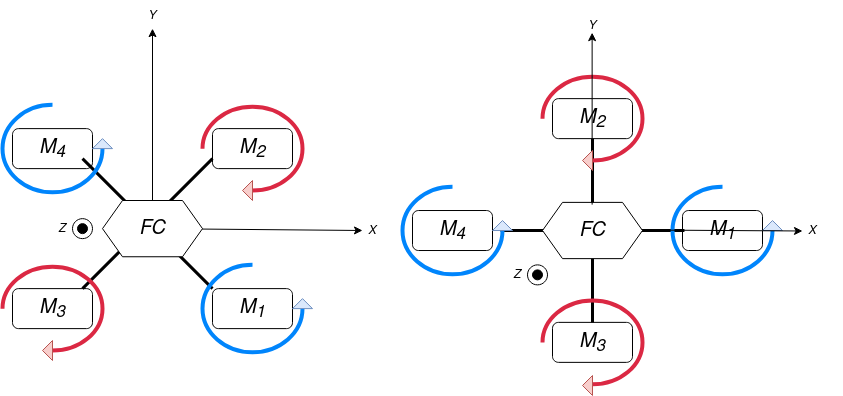
\includegraphics[width= \linewidth]{figures/quad.png} 
	\caption{"X" and "+" configuration of a quadrocopter with the motors ($M_1 ... M_4$), the flight controller($FC$) and the rotational movement of the corresponding propeller (red clockwise, blue counterclockwise)}
	\label{fig:quad}
\end{figure}

A quadrocopter is a modern aircraft with a wide range of applications which is immensely popular in modern society. 
Typically, a quadrocopter can be described as an aircraft with 6 degrees of freedom (DOF), 
which consist of 3 translational and 3 rotational DOF around the $x,y,z$ axis with the corresponding angle $\Theta, \phi, \psi$. \\
As a consequence it has the ability to maneuver in 3D space with all possible rotations, 
although some rotations like a rotation of $\pi$ around the $x$ Axis ($\Theta = \pi$) may cause an inevitable crash. \\
The heart of the quadrocopter is the flight controller ($FC$) which consists of sensors and a MCU that controls the flight. 
Besides, the aircraft possesses 4 motors with corresponding propellers. 
There are different configurations how the motors can be placed in relation to the axis. 
The two most common configuration, the "X" and "+" configuration, can be seen in the above figure. 
The "+" configuration places the motors alongside the x and y-axis. In contrast to that, each motor has an angle of $45^{\circ}$ to the x and y-axis in the "X" configuration.\\
Each of the propeller can be described by their rotational speed $\omega_i$ with $i \in [1...M]$ and spins either clockwise or counterclockwise (\cref{fig:quad}). 
Depending on the configuration of the motors,
the rotation speeds directly influence the \emph{Euler Angles} $\Theta, \phi, \psi$ and
the upward thrust $\tilde{f}$. However, hereafter the most common "X" configuration is used to explain the quadrocopter further.

\newpage 


\subsection{Quadrocopter Flight Dynamics}
The quadrocopter flight dynamics mainly depend on the rotational speed $\omega_i$ of the propellers, 
which mainly produce the translational  and rotational movements. 
Besides, the thrust factor $b$ which is a constant that mainly consists of propeller geometry and frame characteristics also influences the movement. 
Depending on the different $\omega_i, b$ an upward thrust $\tilde{f}$ and a rotation $u_{\Theta}, u_{\phi}, u_{\psi}$ is produced 
that can be comprehended with the following set of formulas:

\begin{align}
	u_{\tilde{f}} &= b \cdot \sum_{i=1}^{4}\omega_i^2 = b \cdot ( \omega_1^2 + \omega_2^2 + \omega_3^2 + \omega_4^2)\label{form:quad}\\
	u_{\Theta} &= b \cdot (\omega_1^2 - \omega_2^2 + \omega_3^2 - \omega_4^2) \label{form:quad2}\\
	u_{\phi} &= b \cdot (\omega_1^2 + \omega_2^2 - \omega_3^2 - \omega_4^2)\label{form:quad3}\\
	u_{\psi} &= b \cdot (\omega_1^2 - \omega_2^2 - \omega_3^2 + \omega_4^2)\label{form:quad4}
\end{align}

\subsubsection{Hover, Rise \& Fall} \label{sec:hover}
\emph{Hovering} can be described as holding a pose $p_{3D} = (x_p, y_p, z_p)$ above the ground, 
rising can be seen as increasing $z_p$ and falling as decreasing $z_p$. 
Therefore, the quadrocopter should not have a rotation on $x,y,z$ axis and mainly depends on \cref{form:quad}.  \\
The product of the thrust factor $b$ and the sum of the squared rotational speeds produces an upward thrust $\tilde{f}$. 
In order to hover equal rotational speeds must be applied to each motor/propeller in order to avoid a rotational movement, because:

\begin{align}
	u_{\Theta} &= b \cdot (\omega_1^2 - \omega_2^2 + \omega_3^2 - \omega_4^2) = b \cdot 0 = 0\\
	u_{\phi} &= b \cdot (\omega_1^2 + \omega_2^2 - \omega_3^2 - \omega_4^2) = b \cdot 0 = 0\\
	u_{\psi} &= b \cdot (\omega_1^2 - \omega_2^2 - \omega_3^2 + \omega_4^2)	= b \cdot 0 = 0
\end{align}
Since all rotational movements null itself, there is only an upward thrust as aerodynamic effect.
Depending on the upward force $F$ and gravitational Force $G$ the thrust produces the already mentioned movements:

\begin{itemize}
	\item $F < G$: Fall
	\item $F = G$: Hover
	\item $F > G$: Rising 
\end{itemize}

\newpage

\subsubsection{Roll}
\begin{figure}
	\centering
	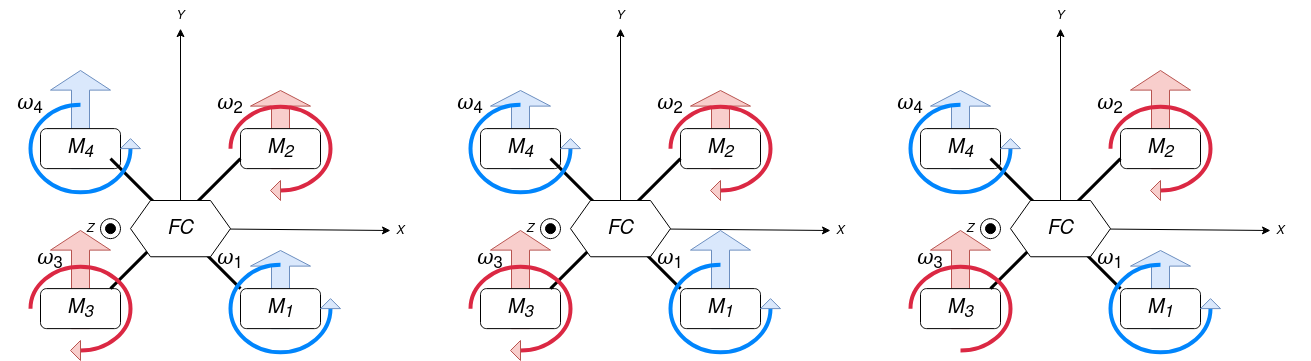
\includegraphics[width=\linewidth]{figures/move.png}
	\caption{Visualization of Roll, Pitch and Yaw rotational movement (from left to right) and the corresponding difference in the rotational speed $\omega_i$}
	\label{fig:move}
\end{figure}
In order to \emph{roll} (rotation around $y$ axis) the thrust on one side has to be greater than on the other side. For example,
increasing $\omega_3, \omega_4$ would lead to uneven distributed thrust. 
The left side of the aircraft experiences more thrust (\cref{fig:move}) and as a consequence the aircraft experiences a torque about the y-axis.
\cref{form:quad2} to \cref{form:quad4} also shows this aerodynamic effect:

\begin{align*}
	\omega_3^* &= \omega_4^* = n \cdot \omega_1 = n \cdot \omega_2 \qquad \qquad \quad \enspace  n > 1\\
	u_{\Theta} &= b \cdot ((\omega_1)^2 - (\omega_2)^2 + (\omega_3^*)^2 - (\omega_4^*)^2) = 0\\
	u_{\phi} &= b \cdot ((\omega_1)^2 + (\omega_2)^2 - (\omega_3^*)^2 - (\omega_4^*)^2) < 0 \\
	u_{\psi} &= b \cdot ((\omega_1)^2 - (\omega_2)^2 - (\omega_3^*)^2 + (\omega_4^*)^2)	= 0 \\
	u_f &= b \cdot ((\omega_1)^2 + (\omega_2)^2 + (\omega_3^*)^2 + (\omega_4^*)^2) > 0 
\end{align*}
\newline
Analogue a roll to the other side can be accomplished by increasing $\omega_1, \omega_2$, then $u_{\phi} > 0$. 
Since the pairs ($\omega_1, \omega_2$) and ($\omega_3, \omega_4$) each have one propeller that spins clockwise and one propeller that spins counterclockwise, 
the total torque of the quadrocopter does not change.\\
\cref{form:quad} shows that there still is an upward thrust, but due to the rotation of the aircraft the thrust force $F$ has a component in $x$ direction. 
This results in a translational movement along the $x$ axis.

\newpage

\subsubsection{Pitch}

A \emph{pitch} movement around $x$ axis works similar to a roll movement, 
just with another motor pair. 
In this case, the thrust at the front or at the back has to increase. 
For example, increasing $\omega_3, \omega_1$ would lead to a bigger thrust at the back 
and the corresponding torque (\cref{fig:move}). \cref{form:quad2} to \cref{form:quad4} also shows this aerodynamic effect:

\begin{align*}
	\omega_3^* &= \omega_1^* = n \cdot \omega_4 = n \cdot \omega_2 \qquad \qquad \quad \enspace  n > 1\\
	u_{\Theta} &= b \cdot ((\omega_1^*)^2 - (\omega_2)^2 + (\omega_3^*)^2 - (\omega_4)^2) > 0\\
	u_{\phi} &= b \cdot ((\omega_1^*)^2 + (\omega_2)^2 - (\omega_3^*)^2 - (\omega_4)^2) = 0 \\
	u_{\psi} &= b \cdot ((\omega_1^*)^2 - (\omega_2)^2 - (\omega_3^*)^2 + (\omega_4)^2)	= 0 \\
	u_f &= b \cdot ((\omega_1^*)^2 + (\omega_2)^2 + (\omega_3^*)^2 + (\omega_4)^2) > 0 
\end{align*}
\newline
Analogue a roll to the other side can be a done by increasing $\omega_2, \omega_4$, then $u_{\Theta} < 0$. 
The total torque also stays the same and the thrust force $F$ gets a component in $y$ direction. This results in a translational movement along the y-axis.


\subsubsection{Yaw}
A \emph{yaw} movement around $z$ axis is not implemented by using a difference in thrust like in the other rotational movements. 
Furthermore, differences in torque are used to accomplish yaw rotations (\cref{fig:move}). \\
For example, if $\omega_1, \omega_4$  increase, the quadrocopter rotates clockwise, 
because the sum of all torques has to stay the same. The external yaw rotation compensates the difference of the sum of the torques of the propeller. 
Besides, \cref{form:quad2} to \cref{form:quad4} shows this aerodynamic effect:

\begin{align*}
	\omega_4^* &= \omega_1^* = n \cdot \omega_3 = n \cdot \omega_2 \qquad \qquad \quad \enspace  n > 1\\
	u_{\Theta} &= b \cdot ((\omega_1^*)^2 - (\omega_2)^2 + (\omega_3)^2 - (\omega_4^*)^2) = 0\\
	u_{\phi} &= b \cdot ((\omega_1^*)^2 + (\omega_2)^2 - (\omega_3)^2 - (\omega_4^*)^2) = 0 \\
	u_{\psi} &= b \cdot ((\omega_1^*)^2 - (\omega_2)^2 - (\omega_3)^2 + (\omega_4^*)^2)	> 0 \\
	u_f &= b \cdot ((\omega_1^*)^2 + (\omega_2)^2 + (\omega_3)^2 + (\omega_4^*)^2) > 0 
\end{align*}
\newline
A counterclockwise yaw rotation can be executed by increasing $\omega_2, \omega_3$, then $u_{\psi} > 0$.
The thrust force $F$ has only a $z$ component. A yaw rotational movement does not result in a translational movement.

 \newpage
 
\subsection{Autonomous Quadrocopter} \label{sec: autoquad}
\begin{figure}
	\centering
	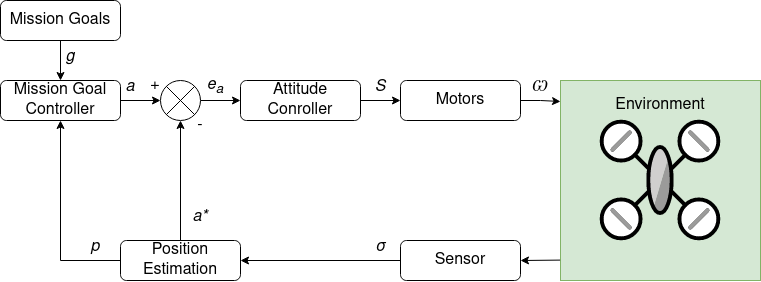
\includegraphics[width=\linewidth]{figures/autoquad.png}
	\caption{Sketch of an autonomous quadrocopter flight control system}
	\label{fig:autoquad}
\end{figure}
Autonomous quadrocopter are especially interesting research topics, because it helps to automate a lot of purposes. 
The general task can be in general defined as calculating the optimal motor signals $S = \{s_1, s_2, s_3, s_4\}$ 
based on the mission goals $g$ and the current pose $p = \{ p_{3D}^*, a^*\}$ in order to achieve a stable flight and satisfy the goals. 
Therefore, it consists of on \emph{inner} and an \emph{outer control loop}.\\
\newline
The inner loop controls the attitude based on the current desired attitude $a$ and the estimated attitude $a^*$. 
By subtracting these the attitude error $e_a$ can be used to calculate the signals $S$, which are most commonly pwm signals. 
The signals are then applied by the motors, which act as actuators and apply a rotational force to the propellers. 
As a consequence the propeller get the rotational speeds ${\Huge \omega } = \{ \omega_1, \omega_2, \omega_3, \omega_4 \}$ 
which directly influence the position of the drone in the environment. 
The state of the drone is captured by the sensor and the corresponding sensor values $\sigma$, which are falsified by noise and offsets. 
They are then used to estimate the attitude. \\
The outer loop controls mission goals based on the prior defined goals $g$ and the current estimated position $p$. 
These inputs are used in order to calculate the desired attitude $a$.\\
\newline
In general Control loops in software are always time discreet. For cascaded controllers like here the inner loop
is running at a higher frequency than the outer loop. 
This is crucial, because attitude control is very time sensitive and has to be implemented in real time. 
A bad or slow attitude control could lead to an unstable flight or in worst case it could crash and therefore automatically erase the possibility to achieve mission goals.\\

\newpage

\subsubsection{Attitude Controller \& Mixing} \label{sec:pid}
Common attitude controller often use \emph{PID controller}  as one of the most essential parts of nearly all commercial quadrocopter flight control. 
PID controller are linear feedback controller with a proportional part, an integral part and a differential part and can mathematically be described in two different ways:

\begin{align}
	u(t) &= K_p \cdot e(t) + K_i \cdot \int_{0}^{t} e(\tau) \enspace d\tau + K_d \cdot \frac{de(t)}{dt} \label{form:pid}\\
	u(t)^* &= K \cdot ( e(t) + \frac{1}{T_n} \cdot \int_{0}^{t} e(\tau) \enspace d\tau + T_v \cdot \frac{de(t)}{dt})
\end{align}
\newline
However, since both are mathematically the same just with other gain definitions \cref{form:pid} will be the relevant one hereafter. 
The control signal $u(t)$ is calculated with the use of the configurable constant gains $K_p, K_i, K_d$, which weigh the different parts of the controller.\\
Within a PID controller the proportional term considers the current error $e(t)$, 
the integral term considers the history of errors by integrating about them and 
the differential term estimates the future error by considering change of the error. 
Since the attitude control is time discrete in software, \cref{form:pid} must be transformed with the use of the sampling time period $\tilde{T}$:

\begin{align}
	u(t) &= K_p \cdot e(t) + K_i \cdot \tilde{T} \cdot \sum_{0}^{t}e(\tau) + K_d \cdot \frac{e(t) - e(t-1)}{\tilde{T}} \label{form:pid2}
\end{align}
\newline
In a quadrocopter there is a PID controller for each of the three axis(roll, pitch, yaw), 
which are all working parallel during an inner loop control cycle. 
Then mixing is used to translate the PID values of each axis to a pwm signal $s_i$ for each motor. 
This process uses a table, which consists of constants that describe the geometry of the frame. 
The throttle coefficient $f'$ and the mixer values of the motor $M_i$ ($m_{i,\phi}, m_{i,\Theta}, m_{i,\psi}$).

\begin{align}
	s_i &= f' \cdot (m_{i,\phi} \cdot u_{\phi} + m_{i, \Theta} \cdot u_{\Theta} + m_{i,\psi} \cdot u_{\psi}) \label{form:mix}
\end{align}
\newline
This implementation is modern state-of-the-art attitude control. It is easy to implement, 
because \cref{form:pid2} and \cref{form:mix} are simple equations and \cref{form:mix} is just in need of some constants. 
In addition, there are not many calculations, so the process can be implemented in realtime. 
Also, this classic approach shows close to ideal performance in stable environments.\\
However, \cite{koch2019reinforcement} shows that with RL an intelligent agent can be trained with the use of PPO (\cref{sec:ppo}) 
that outperforms a classic PID Attitude controller in harsh, unpredictable environments. 
%It also shows that an agent trained with the use of DDPG (\cref{sec:ddpg}) is not good enough for stable attitude control.

\newpage

\subsubsection{Position Estimation}
Position or state estimation can be accomplished in different ways. 
By the use of classic filters the sensor values are more accurately, although there still is a relevant error. 
\emph{Kalman Filters} are the common state-of-the-art solution for position estimation, because they are statistical optimal. 
Although the name suggests otherwise a Kalman Filter is not a classic filter, but a stochastic weighted combination of the state prediction and measurement. \\
At each step, the next position and the next measurement is predicted. 
Based on the prediction of the measurement and the real measurement an innovation is calculated and used in combination with the Kalman Filter Gain $K$ 
to calculate the next state. 
At the same time, the state has a covariance and the covariance of the next state is calculated. 
Then the covariance of the innovation and the Kalman Filter Gain $K$ is calculated and used to correct the covariance of the state.\\
The amount of calculations increases exponentially with the amount of used sensor values. As a consequence,
the use of sensors for the Kalman Filter is limited in realtime tasks. 
In addition, it is in need of linearization. As a consequence there is research to further enhance the filter.
For example, \cite{shi2022deep} shows Deep Kalman Filters, 
which combine the learning ability of deep learning method and the noise filtering ability of the classic Kalman Filter can further enhance trajectory estimation. 
Although it should be mentioned that the mentioned work uses external satellite images of moving targets. So, the use case is quite different, but in theory adaptable. 

\subsubsection{Pathfollowing Controller}
Pathfollowing Controller work in the outer control loop as Mission Goal Controller (\cref{fig:autoquad}) with the goal $g$ typically defined as a set of waypoints $\Lambda = \{\lambda_i \quad i \in [0...n]\}$. 
These waypoints can be defined in different ways:
\begin{itemize}
	\item  $\lambda_i = \{x,y,z\}$: classic point in 3D space
	\item  $\lambda_i = \{x,y,z,\Theta, \phi, \psi\}$: point in 3D space with attitude
	\item  $\lambda_i = \{x,y,z,t\}$: classic point in 3D space with time when it should be reached\\
	$\rightarrow$ would lead to a Trajectoryfollowing Controller
	\item  $\lambda_i = \{x,y,z,\Theta, \phi, \psi, t\}$: point in 3D space with attitude and time\\
	$\rightarrow$ would lead to a Trajectoryfollowing Controller
\end{itemize}
At the moment there is a wide range of different approaches for this task. Typically,
either straight line paths or circular orbit paths are implemented, depending on the use case.\\
For example, \cite{nelson2007vector} implemented a \emph{Vector Field Pathfollowing} with promising results, 
although \cite{6669680} shows that this accuracy is combined with large control effort. 
But there is also the possibility to use a PID like implementation or a classic carrot chasing algorithm.\\
%In this work, the implementation of Reinforcment Learning for a robust Pathfollowing Controller will  be explained and evaluated.

\newpage

%%%%%%%%%%%%%%%%%%%%%%%%%%%%%%%%%%%%%%%%%%%%%%%%
\section{Reinforcement Learning Basics}
\begin{figure}
	\centering
	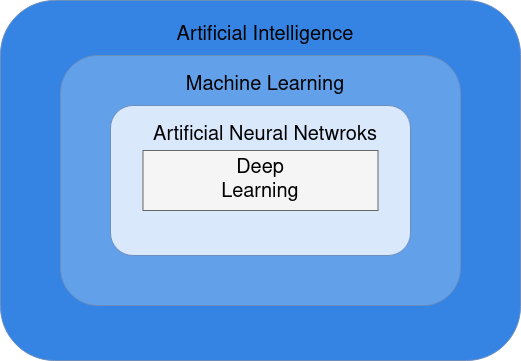
\includegraphics[width= 0.75 \linewidth]{figures/onion.png}
	\caption{Concept onion of Artificial Intelligence \cite{NN}}
	\label{fig:onion}
\end{figure}
In modern society the field of artificial intelligence is increasingly recognized and used. 
Be it transformer technologies such as ChatGPT or classic deep learning, artificial intelligence has applications in a variety of different fields of science and everyday life.\\
Therefore, before explaining RL the different terms and aspects of the different methods should be distinguished.\\
\emph{Artificial Intelligence} refers to an area in computer science, 
which deals with the simulation and application of behaviour that humans would define as intelligent. 
Although it is hard to define intelligence, there are some easy recognizable symptoms such as solving problems independently or human like interactions. 
The \emph{Turing Test} \cite{TT} represents an operative definition of intelligence. 
To sum it up, an algorithm passes the test, if a human, who previously asked written questions, 
can not determine whether the answer is given by the algorithm or a human. 
In order to pass this test, the algorithm is in need of different things:
\begin{itemize}
	\item \emph{Natural Language Processing (NLP)}: processing, interpretation, generation and output of natural language
	\item \emph{Knowledge Representation}: understanding the content of the question
	\item \emph{Logical Close}
	\item \emph{Machine Learning (ML)}: adapt to new context, recognize structures
\end{itemize}
With these definitions and \cref{fig:onion} it is easy to locate RL, 
which is an area of machine learning and often uses artificial neural networks in order to satisfy the designated task.

\newpage

\subsection{Classification of Machine Learning Areas}
\begin{figure}
	\centering
	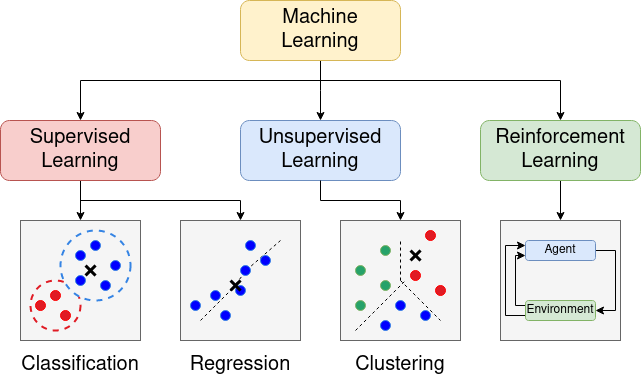
\includegraphics[width=\linewidth]{figures/mlpng.png}
	\caption{The main learning strategies of machine learning including the related approaches like classification and regression under the Supervised Learning, clustering under the Unsupervised Learning and a sketch of the Reinforcement Learning concept}
	\label{fig:ml}
\end{figure}
In general Machine Learning is seen as a subfield of artificial intelligence (\cref{fig:onion}), 
that deals with generating knowledge based on experience. 
ML programs learn patterns based on training data and then can perform tasks without being explicitly programmed to do so by generalizing unknown examples. 
\subsubsection{Supervised Learning}
\emph{Supervised Learning} builds a model based on labelled data, which contains the input and the matching output.
By iterative optimization supervised learning algorithms learn a function that can be used to predict the output associated with inputs. 
If learned correctly it also presents the output for inputs that were not a part of the training data set. 
In this case, the outputs should be analogue to the outputs of similar training data.\\
The two most common types of Supervised Learning algorithms are \emph{Classification} and \emph{Regression} (\cref{fig:ml}).\\
Classification algorithms are in need of outputs that are restricted to a limited set of categories. 
After training the model can determine which category belongs to a certain input.
Regression algorithms learn a model to estimate the relationship between a dependent and one or more independent variable 
and are used when the outputs may have a numerical value within a defined range.\\

\subsubsection{Unsupervised Learning}
\emph{Unsupervised Learning} builds a model with unlabeled data, which only contains the input data. 
In contrary to Supervised Learning the data set does not contain a preferred output for the given inputs. 
Unsupervised Learning aims at discovering a distribution of the data in order to gain new knowledge.\\
\emph{Clustering} (\cref{fig:ml}) discovers clusters within the given data and can therefore predict for new inputs the related cluster.

\subsubsection{Reinforcement Learning}
\emph{Reinforcement Learning} is an area of ML designated to modelling decision-making by finding a way to take an action in en environment in order to maximize the sum of rewards. 
It has proven successful in a wide range of different problems like game theory, control theory or swarm intelligence. 
The main difference of RL to the already mentioned areas of ML is that the action affects the environment and therefore the observation it receives. 
Also, it learns by the use of a reward signal.\\
The \emph{intelligent agent} is the decision maker and typically implemented with the use of a \emph{Neural Network} (\cref{sec:NN}). 
\cref{fig:rl} shows the basic idea: at each time step $t$ the agent takes an action $a_t$ based on the prior observed state $s_{t-1}$. 
Based on how good the action was he receives a reward $r_{t+1}$ and the new state $s_{t+1}$.
The reward signal can either depend on the state $(s_t)$, the state and the chosen action $(s_t, a_t)$ or the state, 
the chosen action and the transitioned state $(s_t, a_t, s_{t+1})$. It is always numerical and used to optimize the agent.
The environment $\epsilon$ receives at each time step the action $a_t$. 
Then, it simulates the state transition based on its implementation. 
It calculates the reward signal $r_{t+1}$ and returns it alongside with the observed transitioned state $s_{t+1}$. 
It should be mentioned that the observed state $s_t$ must not be the complete intern state of the environment $s_t^*$. 
Furthermore, it is only an observation and also can be defined as $o_t$.  
In general, the environment can be modelled with the use of a \emph{Markov Decision Process}.

\begin{figure}
	\centering
	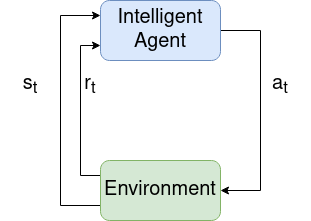
\includegraphics[width=0.4\linewidth]{figures/rl.png}
	\caption{The basic concept of RL: the agent takes an action based on the observed state and receives a numerical reward at each time step}
	\label{fig:rl}
\end{figure}

\newpage

\subsection{Markov Decision Process} \label{sec:MDP}
A \emph{Markov Decision Process} (MDP) is a time discreet stochastic control process, which constitutes a mathematical framework for modelling decision-making. 
A MDP is formally defined as a 5-Tupel $(S,A,R,P,p_0)$, where:
\begin{itemize}
	\item $S$ is the state space with the states $s_i \in S$ 
	\item $A$ is the action space with the actions $a_i \in A$
	\item $R$ is the reward function, mapping $S \times A \times S \to \mathbb{R}$\\
				with:\\
				$r_{t+1} = R(s_t)$, $r_{t+1} = R(s_t, a_t)$ or $r_{t+1} = R(s_t, a_t, s_{t+1})$
	\item $P$ is the state transition probability function mapping $T(s_t,a_t,a_{t+1}) \sim Pr(s_{t+1}|s_t,a_t)$
	\item $p_0$ is the starting state distribution 
\end{itemize}
The state space $S$ is a set of states $s$ and may be discreet or continuous. 
Analogue, the action space $A$ may be discreet or continuous. 
If there are final states the MDP is called \emph{finite MDP}, else \emph{continuing MDP}. \\
The reward function always returns a numerical reward. 
Like previously mentioned the reward may only depend on the state $s_t$ or state and action $a_t$, or state, action and transitioned state $s_{t+1}$. \\
When transitioning from one state to the next, the transitioning must not be deterministic. 
$P$ maps a probability to a transition $T(s_t,a_t,a_{t+1})$ from state $s_t$ to state $s_{t+1}$ by choosing the action $a_t$. 
But there also may be deterministic transitions. 
Then there only is one possible state to transition to and taking the related action will result in this transition with a probability of 1. 
In addition, the transitions always support the Markov property, that defines that transitions only depend on the most recent state and action. 
So the prior states $s_0 ... s_{t-1}$ are irrelevant for the current transition.\\
In addition, the starting state distribution defines which states may be the first state $s_0$. \\
\newline
By modelling a RL problem as a MDP, there is a mathematical basis to optimize the decision-making. 
Further, it defines the possible states and actions. Choosing a good reward function is the key to influence the decision-making. 
For example, by penalizing the transition to a bad state the agent will learn to avoid choosing the matching action. 
Analogue, a big positive reward can influence the decision-making.

\newpage

\subsubsection{Visualization}
\begin{figure}
	\centering
	\includegraphics[width=\linewidth]{figures/visMdp.png}
	\caption{Visualization of a simple MDP with 4 states ($s_0, s_1, s_2, s_3$) (blue nodes), 2 actions ($a_0, a_1$), 
	state-action edges (green) and action-state edges (dark red) containing a tuple (possibility, reward)}
	\label{fig:vismdp}
\end{figure}
A Markov Decision Process can be visualized with the help of a directed transition graph. 
The graph posses state nodes and action nodes. 
Each state node is connected with $n \in \mathbb{N}_0$ actions with directed state-action edges. 
Each action node is connected with $k \in \mathbb{N}$ states with action-state edges, that posses a probability $\alpha_i$. 
Since after taking in action there must be a transition, it follows that the sum of all the outgoing action-state edge probabilities must be equal to 1:

\begin{align}
	\sum_{i=0}^{k} \alpha_i &= 1
\end{align}
\newline
It is also possible that there is a state-action edge from state node $s_k$ to action node $a_n$ and an action-state edge from $a_n$ back to $s_k$. 
It is equivalent to taking an action that may cause no transition at all and the state stays the same. In addition, the graph may possess starting and ending states.\\
For example, \cref{fig:vismdp} shows a finite MDP with 4 states (blue nodes). 
$S_2$ is defined as starting state and since no action can be taken in state $s_3$, this is an ending state. 
If a state possesses multiple state-action edges like $s_0$ a decision has to be made. 
After choosing an action there may be multiple action state edges like action $a_1$ from state $s_0$. 
In this example there is a state transition to $s_1$ with a probability of $1-\beta$ that succeeds in a numerical reward of $-3$. 
Also, there is the possibility of $\beta$ to transition into $s_0$ which causes a reward of $1$.

\newpage

\subsection{V,Q Function \& The Bellman Equations}
In order to further define how the agent learns, there are a couple of functions, equations and helpful definitions. 
The \emph{policy} $\pi$ defines which action should be taken based on the current state and the \emph{trajectory} $\tau$ 
defines different possible sequence of transitions inside the MDP. 
In order to find the optimal trajectory there are different metrics defining an expected value to each state (\emph{V Function} \cref{sec:V}) and each state-action pair (\emph{Q Function} \cref{sec:Q}). 
With these functions different policies can be evaluated. 

\subsubsection{Policy}
The policy $\pi$ is a mapping from the state space $S$ to the action space $A$. Formally this mapping is described as
\begin{align*}
	S \to \mathbb{P}(A, \pi (a_t,s_t))
\end{align*}
\newline
and defines the probability of choosing the action $a_t$ in state $s_t$.\\
In many RL Algorithms \emph{Neural Networks} (\cref{sec:NN}) will be used to model the policy with 
the goal to approximate an optimal policy $\pi^*$ that maximizes the expected reward:
\begin{align*}
	\pi^* = \underset{\pi} {\arg \max} J(\pi)
\end{align*}

\subsubsection{Trajectory}
A sequence of states $s_0 ... s_{T+1}$ and the matching action $a_0 ... a_T$ is called a trajectory $\pi$ with the amount of steps $T$.
For example there could be the trajectory $\tau_1 = (s_2, a_0, s_0, a_1, s_1)$ for the visualized MDP (\cref{fig:vismdp}) with $T=2$ steps:
Since $s_2$ is defined as a starting state it is always the first state of the trajectory. 
By choosing $a_0$ there is a state transition to state $s_0$. Then there is a transition to state $s_1$ by choosing the action $a_1$. 
This trajectory $\tau_1$ could be achieved with the policy $\pi_1$ with $\pi_1(a_0|s_2) = 1, \pi_1(a_1|s_0) = 1$. 
This policy literally defines that in the state $s_2$ always the action $a_0$ should be taken and in state $s_0$ always the action $a_1$.
Further there can be described a probability that this trajectory $\tau$ occurs under the policy $\pi$.

\begin{align}
	P(\tau| \pi) = p_0(s_0)  \prod_{t=0}^{T-1} P(s_{t+1}s_t,a_t|) \pi (a_t|s_t) 
\end{align}
\newline
This is basically the product of the probabilities that the policy $\pi$ takes an action and that the action $a_t$ transitions the state to $s_{t+1}$. 
In the above example, this would result in

\begin{align*}
	P(\tau_1|\pi_1) = 1 \cdot \lambda \cdot 1 \cdot (1-\beta) = \lambda \cdot (1-\beta)
\end{align*} 

\newpage

\subsubsection{Discounted \& Undiscounted Reward}
In \emph{finite}, episodic MDPs with ending states, the sum of the rewards is easy to calculate for a trajectory $\tau$ with the use of the amount of steps $T$.

\begin{align}
	R(\tau) = \sum_{t=0}^{T-1}r_{t+1}
\end{align}
\newline
It was already discussed in \cref{sec:MDP} that a MDP may be infinite and continuing. 
As consequence the undiscounted reward, that was defined in the above may diverge, because there is no ending state. 
In order to counter the diverging of the sum a discount factor $\gamma \in [0...1]$ is used. 
The idea behind is to weigh future rewards. With increasing future step $t$ the weigh factor decreases exponentially. 
As a consequence the sum of the rewards converges and is called discounted reward.

\begin{align} \label{form:direw}
	R(\tau)_t &= \sum_{k=0}^{\infty} \gamma^k \cdot r_{t+k+1} \\
	&= r_{t+1} + \gamma \cdot r_{t+2} + \gamma^2 \cdot r_{t+3} + ... 
\end{align}
\newline
\cref{form:direw} shows how the discounted reward is calculated:\\
Future rewards are weighed with the factor $\gamma^n \quad n \in \mathbb{N}_0$ depending on how many steps they are in the future. 
The special case of $\gamma = 1$ means that the task should be episodic, the case of $\gamma = 0$ results in a greedy implementation, 
where future rewards are not considered at all and the agent learns to always choose the action that implies the highest reward in that step.
With the before mentioned possibility of a transition $\tau$ under the policy $\pi$ an expected reward $J(\pi)$ of a policy can be defined. 
For example in \cref{fig:vismdp} there can be a couple of $T=2$ step trajectories $\tau_i$ with a matching probability and reward $R(\tau_i)$ (\cref{tab:ex}) 
that leads to an expected reward $J(\pi_1)$ of depending on the transition probabilities $\lambda, \beta, \alpha$:
\begin{align*}
	J(\pi_1) = \lambda \cdot \beta - 3 \cdot \lambda \cdot (1-\beta)
\end{align*}
\begin{table}
	\centering
	\caption{Example of all two step trajectories with the matching probability, reward and expected reward of the MDP shown in \cref{fig:vismdp}}\label{tab:ex}
	\begin{tabular}{c|c|c|c}
		$\tau$ & $P(\tau|\pi)$ & $R(\tau)$ & $J(\tau)$\\
		\hline
		$(s_2,a_0,s_3)$ & $(1-\lambda) $ & $0$ & $0$\\
		$(s_2,a_0,s_0,a_1, s_0)$ & $ \lambda \cdot \beta$ & $1$  & $\lambda \cdot \beta$\\
		$(s_2,a_0,s_0,a_1, s_1)$ & $\lambda \cdot (1-\beta)$ & $-3$ & $-3 \cdot \lambda \cdot (1 - \beta)$\\
	\end{tabular}
\end{table}

\newpage

\subsubsection{V-Function} \label{sec:V}
A vast majority of \emph{Reinforcement Learning Algorithms} try to estimate a \emph{Value Function} in order measure how good it is 
to be in a state $s_t$ under a matching policy $\pi$. 
The V Function calculates the expected return $J(\pi)$ with the starting state $s_t$ and acting accordingly to the defined policy:

\begin{align}
	V^{\pi}(s) &= \mathbb{E}_{\tau \sim P(\cdot|\pi)}[R(\tau)|s_0=s] \\
	&= \mathbb{E}[\sum_{k=0}^{\infty}\gamma^k r_{t+k+1|s=s_t}]
\end{align}
\newline
In addition, an \emph{optimal Value Function} (\cref{eq:opv}) can be defined and used in order to calculate an optimal policy:

\begin{align}\label{eq:opv}
	V^*(s) &= \max_{\pi} V^{\pi}(s)
	= \max_{\pi} \mathbb{E}_{\tau \sim P(\cdot|\pi)}[R(\tau)|s_0=s]
\end{align} 

\subsubsection{Q-Function} \label{sec:Q}
The \emph{Q Function} (action-value function) is defined quite similar to the Value Function but instead of starting in a state, 
the Q Function starts in a state-action pair and then takes actions according to the chosen policy. Therefore, it is also mathematically defined as the expected reward:

\begin{align}
	Q^{\pi}(s,a) &= \mathbb{E}_{\tau \sim P(\cdot|\pi)}[R(\tau)|s_0=s, a_0=a]
\end{align}
\newline
Analogue to the V Function, an \emph{optimal Q Function} can be calculated by taking the maximal expected reward.

\begin{align} \label{eq:opq}
	Q^*(s,a) &= \max_{\pi} Q^{\pi}(s)
	= \max_{\pi} \mathbb{E}_{\tau \sim P(\cdot|\pi)}[R(\tau)|s_0=s, a_0=a]
\end{align}
\newline
With the help of the optimal Q Function the optimal action $a$ for every state can be chosen by comparing 
their optimal Q values and used to construct an optimal policy $\pi^*$. 
If the MDP has discreet actions and states this is no problem and then called \emph{Tabular Reinforcement Learning}. 
For more complex  MDPs RL algorithms that use NN can be used. Probably the best known algorithm of this kind is 
\emph{Deep Q Learning} \cite{pmlr-v120-yang20a} which estimates the Q Function with the use of a behaviour and a target policy. 
These policies are implemented with the use of Neural Networks.

\newpage

\subsubsection{The Bellman Equations}
The \emph{Bellman equations} are the central point of some RL algorithms. It parts the V and Q function into two
separate parts consisting of the instant reward and the discounted future values. As an effect it simplifies the computation of the value function. 
Instead of building a sum over multiple time steps, an optimal solution of a complex problem is found by finding optimal solutions for simpler, recursive subproblems.

\begin{align}
	V^{\pi} (s) &= \mathbb{E}_{a \sim \pi (\cdot | S), s' \sim P(\cdot | S,a)} [R(s,a,s') + \gamma \cdot V^{\pi}(s')] \label{eq:beV} \\
	Q^{\pi} (s,a) &= \mathbb{E}_{s' \sim P(\cdot |S,a)} [R(s,a,s') + \gamma \cdot  \mathbb{E}_{a' \sim \pi (\cdot | s')}[Q^{\pi}(s',a')]] \label{eq:beQ}
\end{align}
\newline
\cref{eq:beV} shows the instant reward $R(s,a,s')$ which is computed by calculating the expected value for all possible actions $a$ and all possible transition states $s'$ and the discounted future $\gamma \cdot V^{\pi} (s')$ reward of the values of the possible transition states. Analogue, \cref{eq:beQ} shows the split up of instant reward and future reward for state-action pairs. As a consequence, iterative approaches can be implemented, that possesses the ability to calculate the values of all states or the values of all state-action pairs. 

\subsubsection{The Bellman Equations of Optimality}
It was already discussed how optimal V and Q functions can be calculated and used to determine the optimal actions 
and create an optimal policy(\cref{eq:opv}, \cref{eq:opq}). 
Analogue the \emph{Bellman Equations of Optimality} can be defined with the use of \cref{eq:beV} and \cref{eq:beQ}:

\begin{align}
	V^*(s)  &= \max_a \mathbb{E}_{s' \sim P(\cdot | s,a)} [R(s,a,s') + \gamma \cdot V^*(s')] \label{eq:bopV}\\
	Q^*(s,a) &= \mathbb{E}_{s' \sim P(\cdot | s,a)} [R(s,a,s') + \gamma \cdot \max_{a'} Q^*(s',a')] \label{eq:bopQ}
\end{align}

%\subsubsection{Monte-Carlo \& TD-Sampling}


\newpage
%%%%%%%%%%%%%%%%%%%%%%%%%%%%%%%%%%%%%%%%%%%%%%%%%

\subsection{Neural Networks} \label{sec:NN}
A \emph{Neural Network (NN)} can be described as a reactive computing system that consists of multiple simple \emph{Neurons} that are interconnected. 
Therefore, the output does depend on the inputs and the defined dynamic state response of each neuron. 
NN are inspired by the network of neurons in the human brain which pass information to another with the help of synapses. 
While biological brains are dynamic and analog, NN tend to be static and symbolic.\\
NN have shown to be very useful, because they are universal function approximators. In addition, they are adaptive
and poses the ability to change their structure based on external or internal information that flows threw it. 
They are non-linear and can be used to model complex relationships between inputs and outputs or find specific pattern in data.

\subsubsection{Neuron}
\begin{figure}
	\centering
	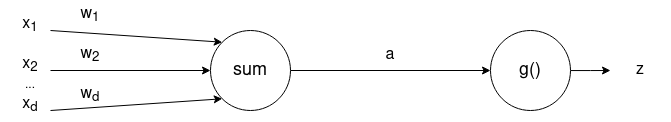
\includegraphics[width=0.8 \linewidth]{figures/neuron.png}
	\caption{The McCulloch-Pitts model of a single neuron uses a weighted sum with the inputs $x_i$ and weights $w_i$ and a 
	non-linear activation function $g()$ in order to compute the output $z$ \cite{10.1063/1.1144830}}
	\label{fig:neuron}
\end{figure}
A Neuron is the basic element of a NN. 
Mathematically a neuron can be seen as a nonlinear function, 
which computes the output $z$ based on a set of inputs $x_i, i \in [1,...,d]$ \cite{10.1063/1.1144830}. 
Further, \cite{mcculloch1943logical} introduced the simple mathematical framework, called the McCulloch-Pits model (\cref{fig:neuron}):

\begin{align}
	a &= \sum_{i=1}^{d} w_i \cdot x_i + w_0 \label{eq: wib}\\
	a &= \sum_{i=0}^{d} w_i \cdot x_i \label{eq:ob}\\
	z &= g(a) \label{active}
\end{align}
\newline
Each input $x_i$ is multiplied with its matching weight $w_i$, 
which is a parallel to synaptic strength in biological networks like brains (\cref{eq: wib}). 
In addition, there is an offset which is called \emph{bias} and is analogue to the firing threshold of a biological neuron. 
By using the bias as additional input and setting it to 1, the sum can be further simplified (\cref{eq:ob}). 
The output of the neuron is then computed by giving it to a non-linear \emph{Activation Function} $g()$.

\newpage

\subsubsection{Activation Function}
\begin{figure}
	\centering
	\begin{subfigure}{0.24\linewidth}
		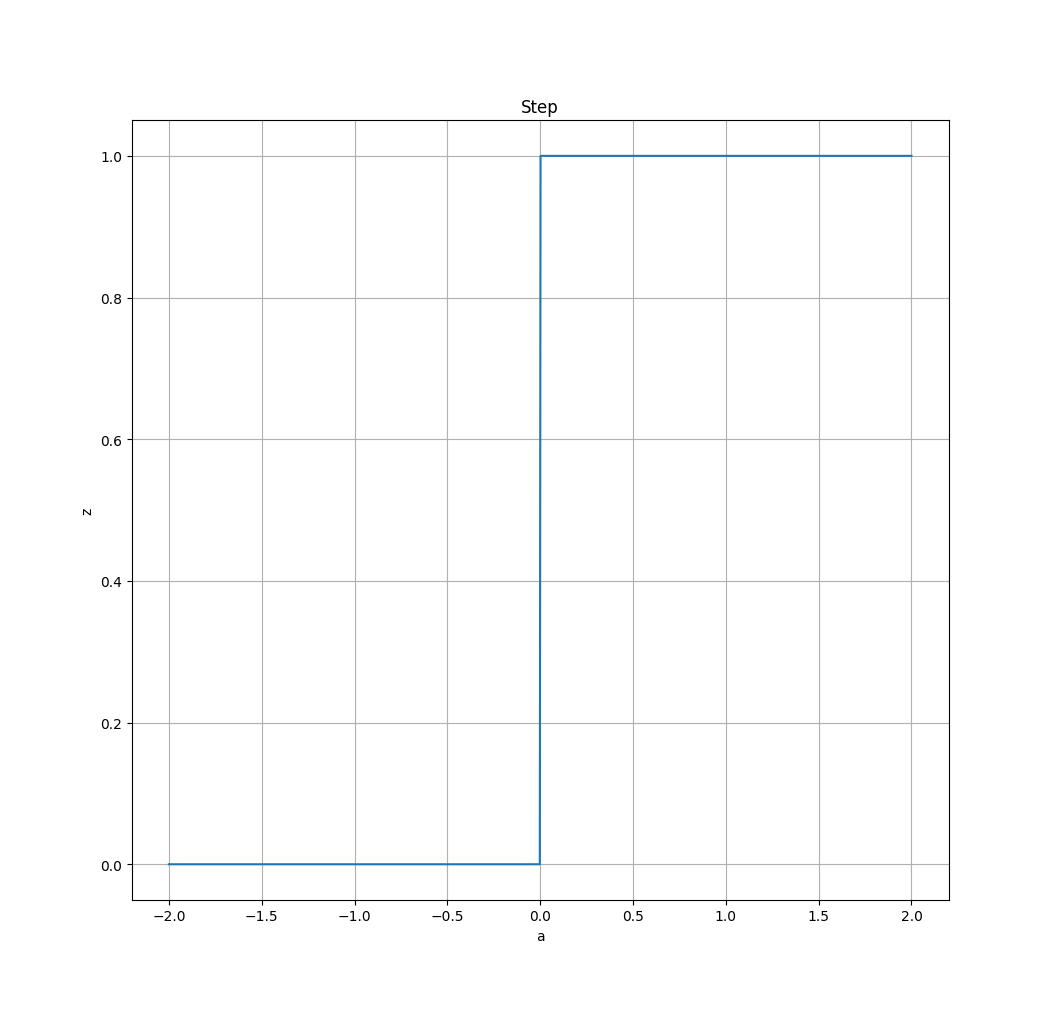
\includegraphics[width=\linewidth]{figures/step.png}
		\caption{Binary Step Function}
	\end{subfigure}
	\begin{subfigure}{0.24\linewidth}
		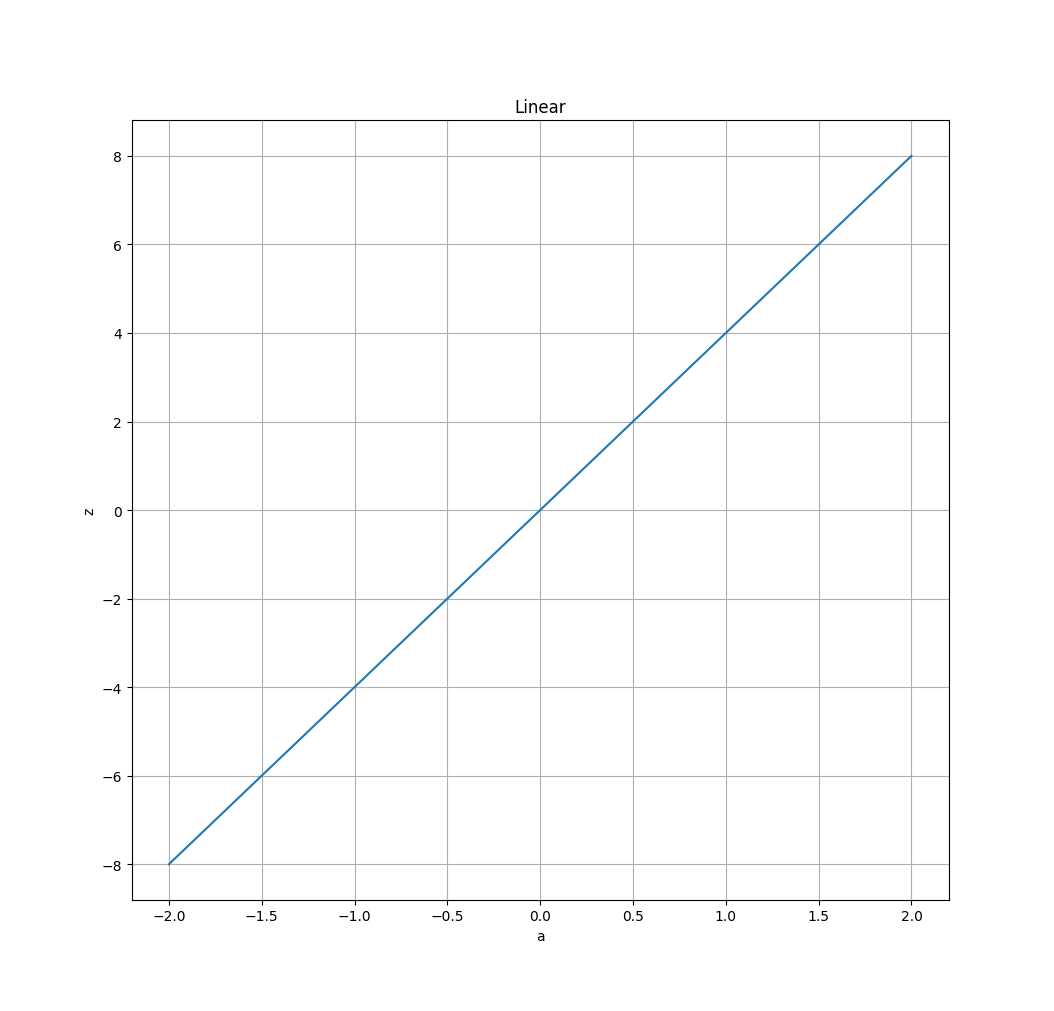
\includegraphics[width=\linewidth]{figures/linear.png}
		\caption{Linear}
	\end{subfigure}
	\begin{subfigure}{0.24\linewidth}
		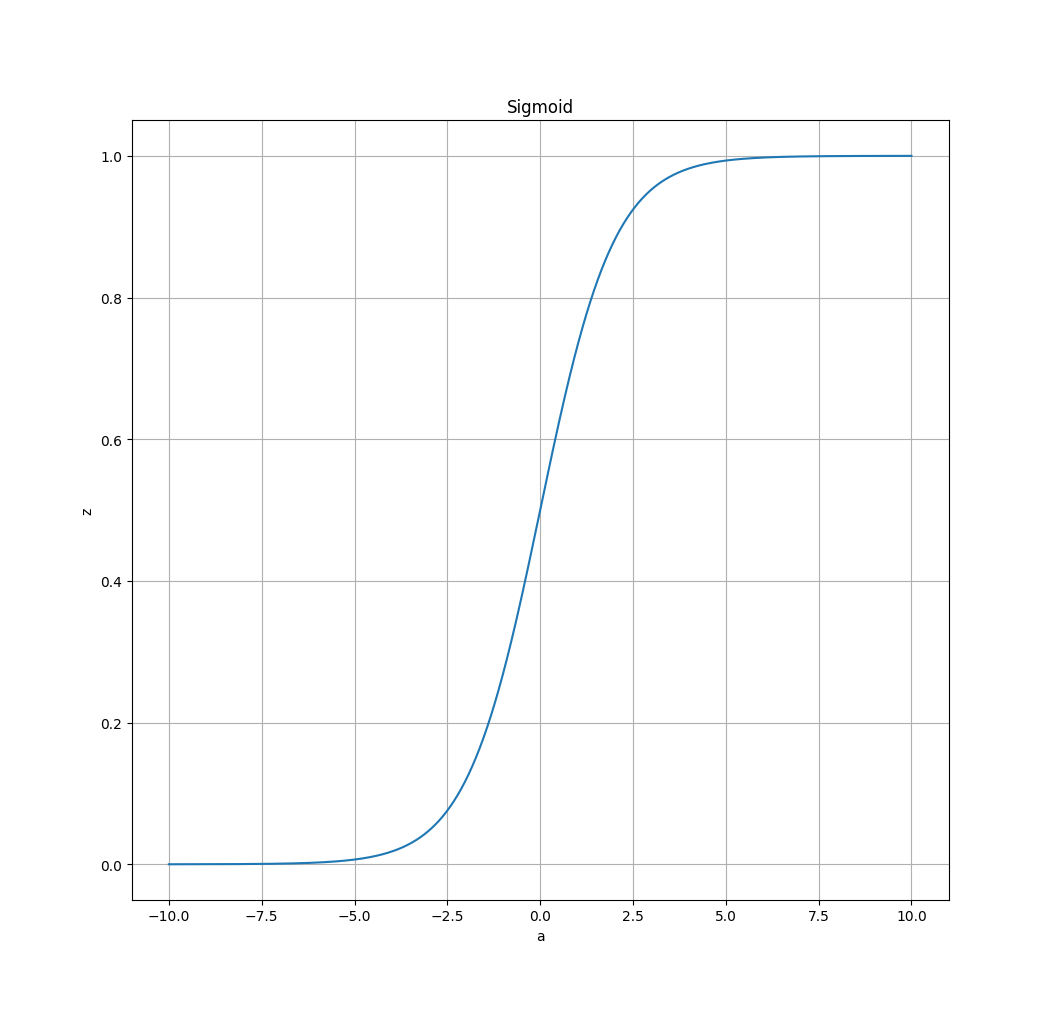
\includegraphics[width=\linewidth]{figures/sigmoid.png}
		\caption{Sigmoid}
	\end{subfigure}
	\begin{subfigure}{0.24\linewidth}
		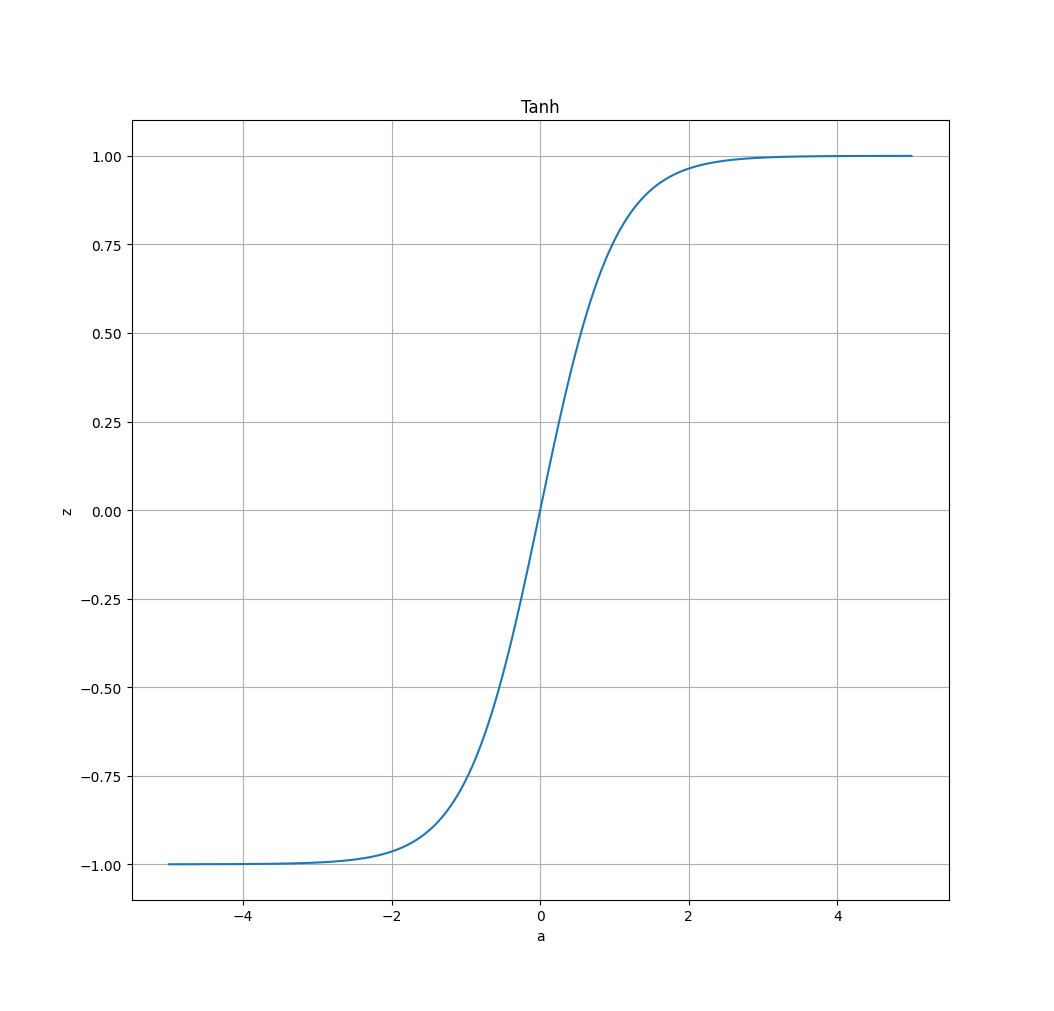
\includegraphics[width=\linewidth]{figures/tanh.png}
		\caption{Tanh}
	\end{subfigure}
	
	\begin{subfigure}{0.24\linewidth}
		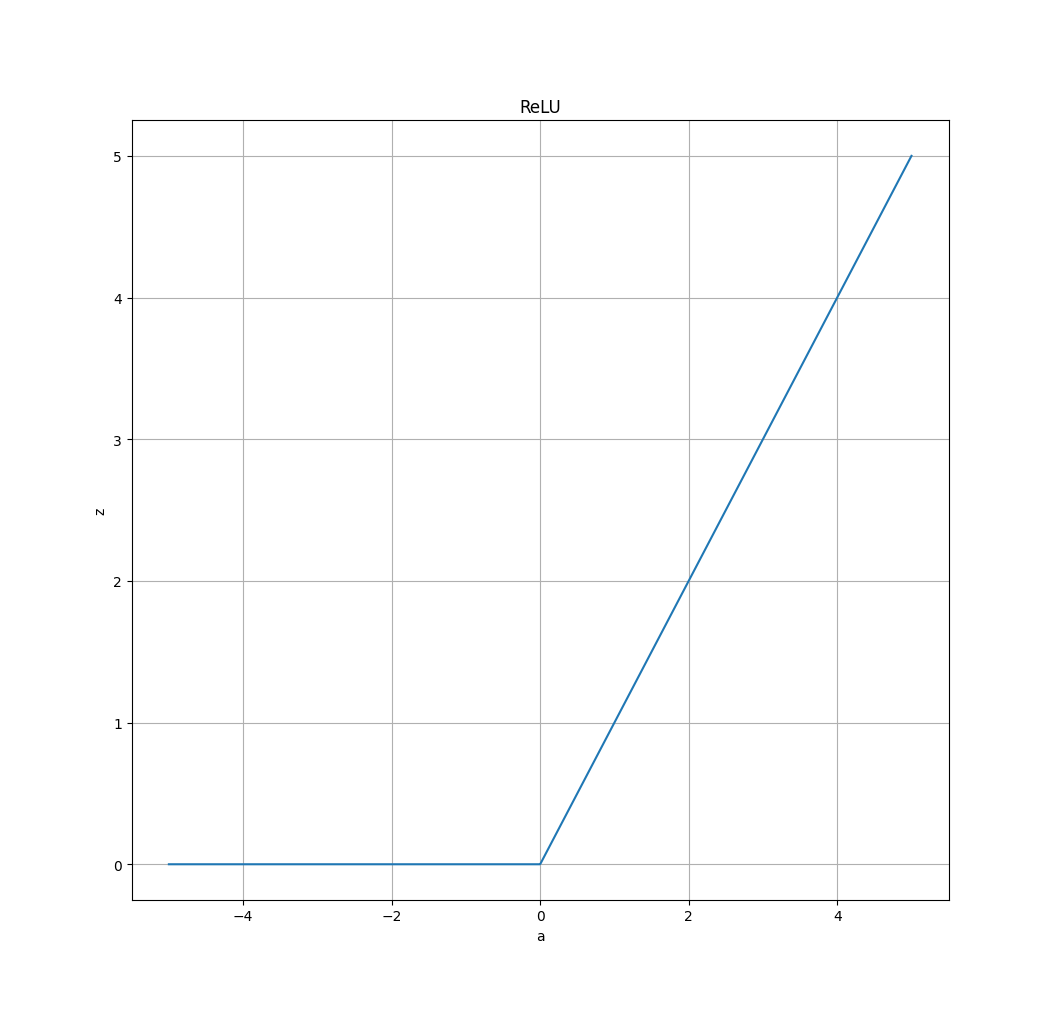
\includegraphics[width=\linewidth]{figures/relu.png}
		\caption{ReLU}
	\end{subfigure}
	\begin{subfigure}{0.24\linewidth}
		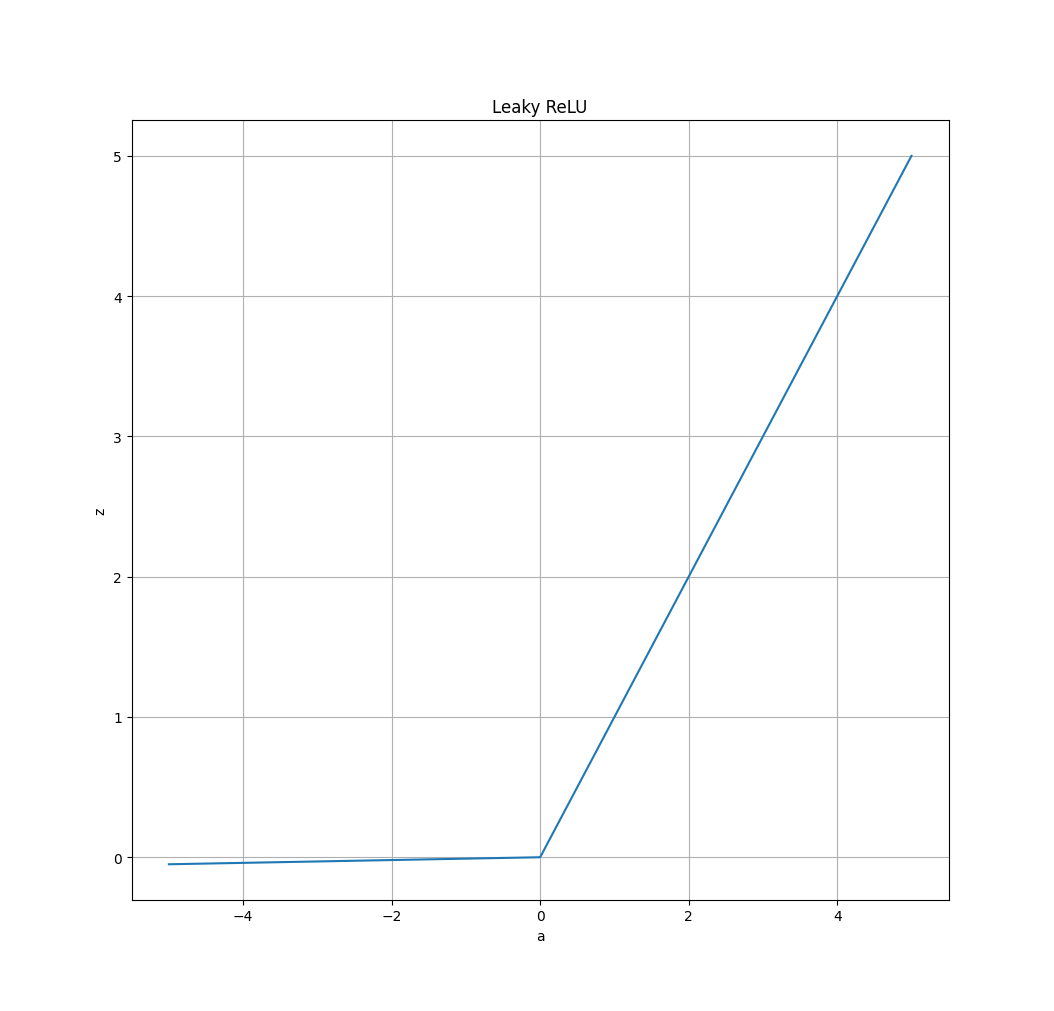
\includegraphics[width=\linewidth]{figures/leakyrelu.png}
		\caption{Leaky ReLU}
	\end{subfigure}
	\begin{subfigure}{0.24\linewidth}
		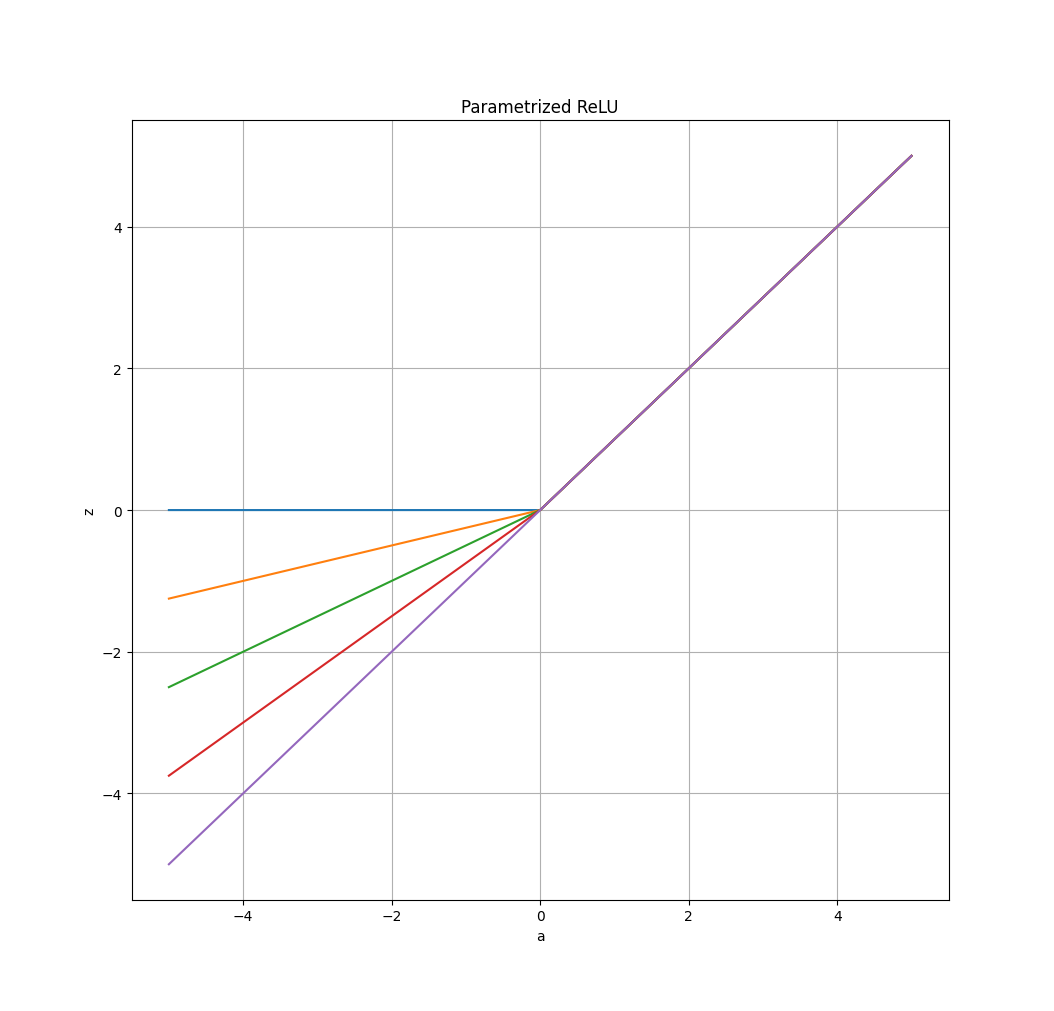
\includegraphics[width=\linewidth]{figures/pararelu.png}
		\caption{Parametrized ReLU}
	\end{subfigure}
	\begin{subfigure}{0.24\linewidth}
		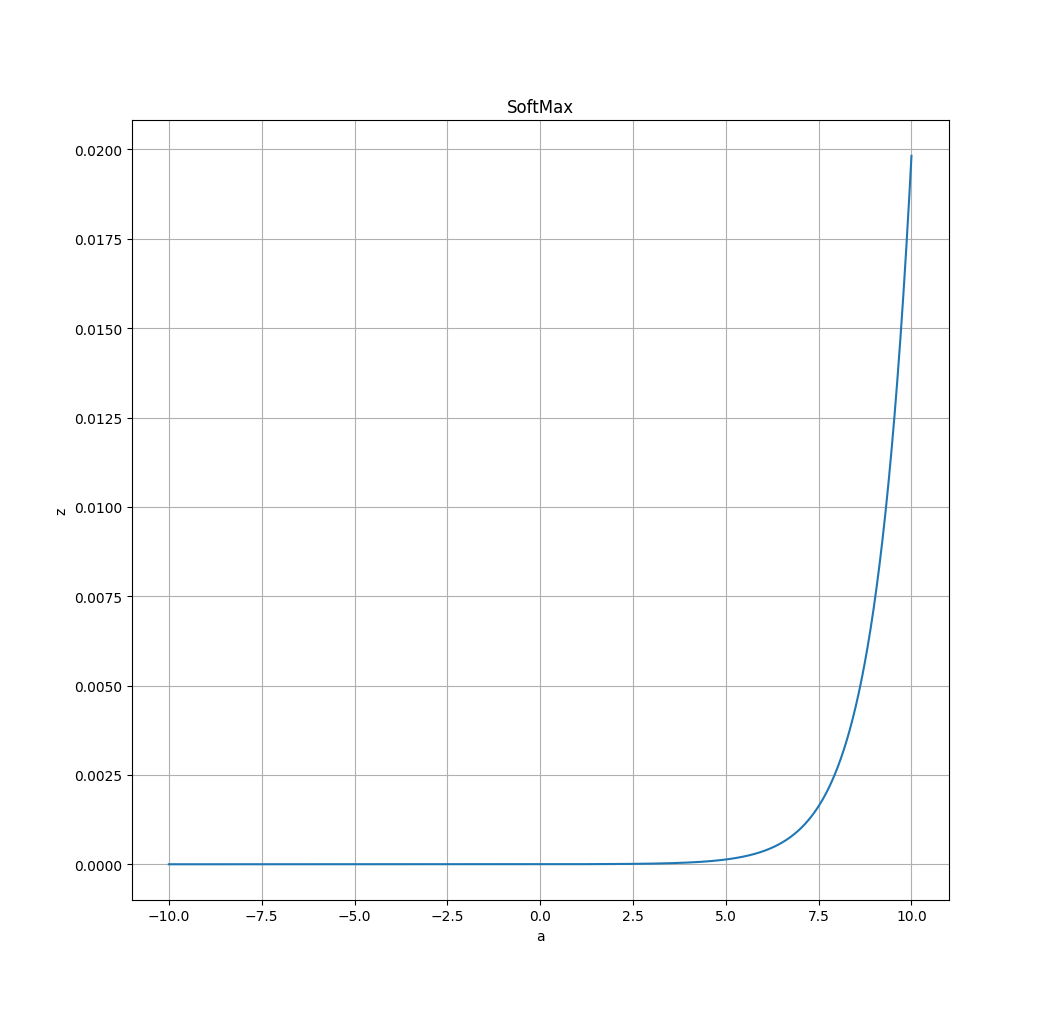
\includegraphics[width=\linewidth]{figures/softmax.png}
		\caption{SoftMax}
	\end{subfigure}
	\caption{8 different Activation Functions.}
	\label{fig:act}
\end{figure}
It was already discussed that NN are universal function approximators and that the neuron consists of a linear sum (\cref{eq:ob}). 
In order to represent nonlinear convoluted functional mappings between input and output, nonlinearity is added to each neuron with an \emph{Activation Function}. 
It is important that these functions are differential in order to implement a back propagation optimization strategy \cite{sharma2017activation}. \\
At the moment, there are different activation functions commonly used (\cref{fig:act}):
\begin{itemize}
	\item Binary Step Function
	\item Linear
	\item Sigmoid
	\item Tanh
	\item ReLU
	\item Leaky ReLU
	\item Parametrized ReLU
	\item SoftMax
\end{itemize} 
Each of this different functions has its advantages. For example, SoftMax is good at multiclass classification problems, 
while Sigmoid is good at binary classification problems. Also, in a NN with ReLU not all neurons are activated at the same time, which increases efficiency.

\newpage

\subsubsection{Simple Feed-Forward Network}
\begin{figure}
	\centering
	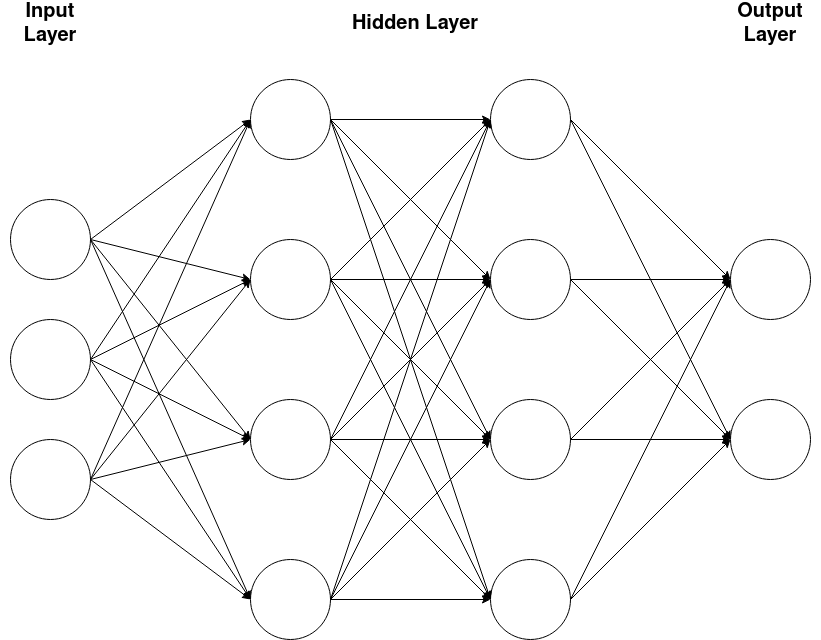
\includegraphics[width=0.55\linewidth]{figures/feedforward.png}
	\caption{Simple Feed-Forward Network with 3 neurons in the input layer, 2 hidden layers with 4 neurons and with 2 layers in the output layer}
	\label{fig:ffn}
\end{figure}
A \emph{Feed-Forward Network} is an artificial network wherein information directly flows forward in one direction from the input to the output. 
In contrast to \emph{Recurrent Neural Networks}, it does not contain cycles of nodes and information can not flow in loops. 
It can be described as a directed graph $G = (V,E,w)$ with neurons as the set of nodes $V$ and the set of edges $E$ with the matching weight $w$ (\cref{fig:ffn}). 
The neurons are grouped into different Layers:
\begin{itemize}
	\item Input Layer: each node receives its input $x$ and calculates the output $z$ with the use of \cref{eq:ob} and passes it to each node of the next layer
	\item Hidden Layer: each node receives its inputs $x_i, i \in [1...d]$ from the $d$ nodes of the previous layer and uses \cref{eq:ob} and the weights $w_i, i \in [1..d]$ in order to calculate the output $z$ and pass it to each node of the next layer
	\item Output Layer: each node receives its inputs $x_i, i \in [1...d]$ from the $d$ nodes of the previous layer and uses \cref{eq:ob} and the weights $w_i, i \in [1..d]$ in order to calculate the output $z$ of the NN
\end{itemize}
The number of hidden layers can differ, likewise the amount of neurons in each layer. 
Due to the structure of neurons even simple Feed-Forward Networks can approximate functions $F: \mathbb{R}^j \to \mathbb{R}^k$, 
where the dimension $j$ equals the amount of nodes in the input layer and $k$ equals the amount of nodes in the output layer.

\subsubsection{Deep Neural Network}
\emph{Deep Neural Networks} differ from the previous mentioned NN in terms of complexity. 
Due to the large amount of neurons and a lot of hidden layers, the NN is able to approximate very complex mappings from the input to the output space.

%%%%%%%%%%%%%%%%%%%%%%%%%%%%%%%%%%%%%

\subsection{State-of-the-Art Algorithms}
\begin{figure}
	\centering
	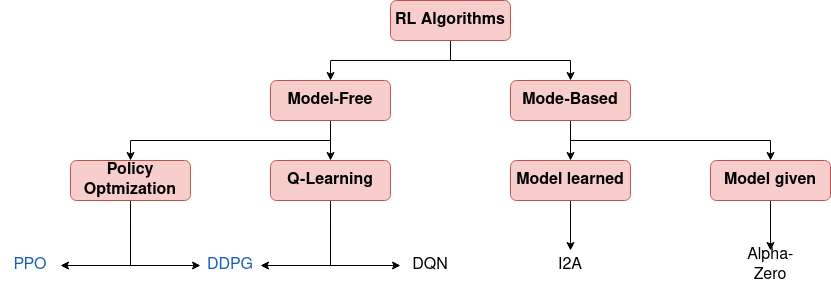
\includegraphics[width=\linewidth]{figures/algo.png}
	\caption{Overview of the different categories of RL algorithms with examples: PPO and DDPG Algorithm colored because they were used in this work.}
	\label{fig:algo}
\end{figure}

Modern state-of-the-art RL algorithms can be divided into different categories (\cref{fig:algo}):\\
\emph{Model-based Algorithms} uses its experience in order to construct a model of the environment by modelling the MDP transitions. 
With the use of this model the optimal actions are chosen for the policy. This category can be further divided into \emph{model learning algorithms} 
like I2A and \emph{model given algorithms} like Alpha-Zero. 
Model learning algorithms observe the trajectory $\tau$ while following a policy $\pi$ and use it in order to learn a dynamics model. 
Then the algorithms plan through the dynamics model in order to choose the actions.
Model given algorithms work quite similar, but the dynamic model is already given.\\
In \emph{Model-free Algorithms} the agent constructs a policy based on trial-and-error experience and can be further divided into 
\emph{Policy Optimization} and \emph{Q-Learning}.
Policy Optimization algorithms like \emph{PPO} (\cref{sec:ppo}) the policy is learned directly. 
In contrast, Q-Learning algorithms like \emph{Deep Q-Learning} learns the Q-function and updates it in order to get an optimal Q-function. 
In addition, there are hybrid algorithms like \emph{SAC} (\cref{sec:sac}) that combines learning the policy function and Q-function.\\
RL algorithms can be further categorized into \emph{on-policy} and \emph{off-policy} algorithms. 
On-policy algorithms use the current optimized policy in order to gain experience that is then used to further optimize the policy. 
In contrast, off-policy algorithms learn from actions that may not be according to the current policy. 
This experience is then used to construct the optimal policy.\\
The algorithms used in this work are part of \emph{Stable Baselines 3}\cite{stable-baselines3}, 
which is a set of reliable implementations of RL algorithms in \emph{PyTorch} that promise efficient learning and a good base to build projects on top of. 
Each of the main state-of-the-art RL algorithms can be found there and used with custom policies, custom environments and custom callback functions. 
In addition, it offers \emph{Tensorboard} support, which is a tool that can be used to visualize the training process.

\newpage
\subsubsection{PPO - Basics} \label{sec:ppo}
PPO algorithms \cite{schulman2017proximal} are a family of policy gradient methods for RL, 
they directly try to improve the policy $\pi$ as much as possible in a single step without stepping to far and avoiding performance collapse. 
It is an \emph{Actor-Critic Method} that approximates the value function $V_{\phi}$ and the policy $\pi_{\Theta}$ with the matching set of parameters $\phi, \Theta$. 
In each step the actor updates the policy parameters and the critic updates the value function parameters. 
In order to measure how good a policy $\pi_{\Theta}$ performs in relation to an old policy $\pi_{\Theta_{old}}$ a surrogate objective is used, 
that keeps the new policies close to the old one:
\begin{align}
	L^{PPO} (\Theta) &= \mathbb{E}_{\tau \sim P(\cdot | \pi_{\Theta_{old}})}[\sum_{t=0}^{T} L(s_t, a_t, \Theta_{old}, \Theta)] \label{eq:obj} \\
	L(s_t, a_t, \Theta_{old}, \Theta) &= \min (
	\frac{\pi_{\Theta}(a_t|s_t)}{\pi_{\Theta_k}(a_t|s_t)} A(s_t, a_t), g(\epsilon, A(s_t, a_t))) \label{eq:obj2}\\
	g(\epsilon, A) &= 
	\left\{
	\begin{array}{ll}
		(1 + \epsilon) \cdot  A  & \mbox{if } A \geq 0\\
		(1 - \epsilon) \cdot A & \mbox{if } A < 0
	\end{array}
	\right. \label{eq:g}
\end{align}
\newline
This surrogate objective mainly depends on the hyperparameter $\epsilon$ which is an upper bound to the distance 
between the policies and the advantage function $A$, that estimates how good an action is compared to the average action for a specific state.\\
\cref{eq:obj} can be explained intuitively by observing a single state-action pair:\\
If the advantage of the state-action pair is positive \cref{eq:obj2} is reduced to
\begin{align}
	L(s_t, a_t, \Theta_{old}, \Theta) &= \min (\frac{\pi_{\Theta}(a_t|s_t)}{\pi_{\Theta_k}(a_t|s_t)}, (1 + \epsilon)) \cdot A(s,a)
\end{align}
Because of the positive advantage the objective will increase with $\pi_{\Theta} (a|s)$, 
but is still limited to $(1 + \epsilon) \cdot A(s,a)$ by the minimum expression. \\
If the advantage of the state action pair is positive \cref{eq:obj2} is reduced to 
\begin{align}
	L(s_t, a_t, \Theta_{old}, \Theta) &= \max (\frac{\pi_{\Theta}(a_t|s_t)}{\pi_{\Theta_k}(a_t|s_t)}, (1 - \epsilon)) \cdot A(s,a)
\end{align}
Because of the negative advantage the objective will increase with the decrease of $\pi_{\Theta} (a|s)$, 
but is still limited to $(1 - \epsilon) \cdot A(s,a)$ by the maximum expression.\\
As a consequence the policy does not profit from changing a lot.\\
PPO is an on-policy algorithm, so the actions are selected according to the latest policy. 
Therefore, the randomness of the action selection decreases over time, which may causes the problem of being trapped in a local optima.

\newpage
\subsubsection{PPO - Algorithm}
The PPO algorithm (\cref{alg:ppo})first initializes the policy and value net with the matching parameters $\Theta_0$ and $\phi_0$.\\
Then the following steps are executed until convergence:\\
By running the current policy $\pi_{\Theta_k}$ a set of Trajectories $D_k$ is collected and the rewards $R_t$ are computed. 
Then the advantage $A$ is computed based in the current value function approximation $V_{\phi_k}$. 
With the use of these values the surrogate objective (\cref{eq:obj}) is calculated and used to update the policy $\pi$. 
Typically, stochastic gradient ascent is used in order to update the policy. At last the value function is updated by using regression on the mean squared error.\\
\newline
Since the release of PPO it is known to be a state-of-the-art algorithm with a good performance that is at least as good as other 
Policy Optimization methods on a variety of environments. In addition, the base algorithm is quite easy to implement.\\
Nevertheless, there are still known problems:\\
The algorithm is quite sensitive to the initialization parameters $\Theta_0, \phi_0$. Like previously mentioned PPO can get stuck in local optima. 
This is the case if there are local optimal actions close to initialization.\\
PPO seems to be unstable when the reward function is not bounded on continuous action spaces. 

\begin{algorithm}
	\caption{Proximal Policy Optimization \cite{schulman2017proximal}}
	\label{alg:ppo}

	Initialize policy parameters $\Theta_0$ and value function parameters $\phi_0$
	
	$k = 0$
	
	\Repeat{convergence}{
		Collect set of trajectories $D_k = \{ \tau_i\}$ by running policy $\pi_{\Theta_k}$
		
		Compute rewards-to-go $R_t$
		
		Compute advantage estimates $A$ based on the current value function $V_{\phi_k}$
		
		Update the policy by maximizing the PPO objective
		\[\Theta_{k+1} = \underset{\Theta}{\arg\max} (\frac{1}{|D_k|} \sum_{\tau_i \in D_k} \sum_{t=0}^{T} \min (
		\frac{\pi_{\Theta}(a_t|s_t)}{\pi_{\Theta_k}(a_t|s_t)} A(s_t, a_t), g(\epsilon, A(s_t, a_t))))\] 
		typically via stochastic gradient ascent
		
		Fit value function by regression on mean-squared error
		\[\phi_{k+1} = \underset{\phi} {\arg \min} (\frac{1}{|D_k|T}
		\sum_{\tau_i \in D_k} \sum_{t=0}^{T} (V_{\phi}(s_t) - R_t)^2)\]
		
		$k += 1$
	}
\end{algorithm}

\subsubsection{SAC - Basics}\label{sec:sac}
\emph{Soft Actor-Critic (SAC)} \cite{haarnoja2018soft} is an off policy RL algorithm that optimizes a stochastic policy. 
It can be categorized as a mixed method between policy optimization and value based methods.
A key feature of SAC is entropy regularization. The policy is trained to maximize a trade-off between expected return and entropy. 
The entropy of a policy can roughly be defined as a metric of measuring the randomness in a policy. 
Increasing the entropy results in more exploration, which accelerates training and can prevent the policy from converging to a bad local optimum.
As a consequence, the RL problem changes to \cref{eq:sac1} with trade-off coefficient $\alpha$ and entropy $H$.
\begin{align}
	\pi^* = \underset{\pi} {\arg \max} \enspace \mathbb{E}_{\tau \sim \pi} [\sum_{t = 0}^{\infty} \gamma^t \cdot 
	(R(s_t, a_t, s_{t+1} + \alpha H (\pi(\cdot | s_t)))] \label{eq:sac1}
\end{align}
As a consequence the definition of the V function and Q function changes to \cref{eq:sacv} and \cref{eq:sacq}.
\begin{align}
	V^{\pi}(s) &= \mathbb{E}_{\tau \sim \pi} [\sum_{t=0}^{\infty} \gamma^t \cdot (R(s_t, a_t, s_{t+1} + 
	\alpha H (\pi(\cdot |s_t))) | s_0 = s] \nonumber\\
	&= \mathbb{E}_{\tau \sim \pi} [\sum_{t=0}^{\infty} \gamma^t \cdot (R(s_t, a_t, s_{t+1} - \alpha \log \pi(a|s)]
	\nonumber \\
	&= \mathbb{E}_{a \sim \pi} [Q^{\pi} (s,a) - \alpha \log \pi(a|s) ]\label{eq:sacv}\\
	Q^{\pi} (s, a) &= 
	\mathbb{E}_{\tau \sim \pi} [\sum_{t=0}^{\infty} \gamma^t \cdot R(s_t, a_t, s_{t+1} + \alpha
	\sum_{t=1}^{\infty} \gamma^t \cdot H(\pi(\cdot | s_t))
	)|s_0 = s, a_0 = a]
	\label{eq:sacq}
\end{align}
SAC solves this new RL problem by learning a policy $\pi_{\Theta}$ and two Q functions $Q_{\phi_1}, Q_{\phi_2}$.
The Q functions are learned by regressing to a single shared target with the loss function seen in \cref{eq:sacloss}.

\begin{align}
	L(\phi_i, \mathcal{D}) &= \mathbb{E}_{(s, a, r, s',d) \sim D} [(y(r,s',d) - Q_{\phi_i}(s,a))^2] \label{eq:sacloss}\\
	y(r,s',d) &= r + \gamma \cdot (1-d) \cdot
	(
	\min_{j=1,2} 
	{{}Q_\phi}_{targ_j}
	(s', \tilde{a}') - \alpha \log 
	\pi_{\Theta} (\tilde{a}'|s') )\label{eq:sactarget}\\
	\tilde{a}' &\sim \pi_{\Theta}(\cdot | s') \nonumber
 \end{align}
 There, $\tilde{a}'$ is the next action. Unlike $r,s'$ the next action is sampled from the policy and not from the replay buffer $\mathcal{D}$.
 \newpage
 The policy should learn to maximize the value of each state $V^{\pi} (s)$ (\cref{eq:sacv}). 
 Therefore, the \emph{reparameterization trick} is used, in which a sample from $\pi_{\Theta}(\cdot | s)$ 
 is collected with the use of a squashed Gaussian policy. 
 There, samples are collected according to \cref{eq:sacsq} and used in the V function (\cref{eq:secv2}). 
 Then, the policy is loss is given by choosing the minimum of the 2 Q function approximators as Q function (\cref{eq:secv3}).
 
 \begin{align}
 	\tilde{a_\Theta} (s, \xi) &= tanh(\mu_{\Theta}(s) + \sigma_{\Theta}(s) \odot \xi) \qquad \xi \in \mathcal{N}(0,I) \label{eq:sacsq}\\
 	V^{\pi} (s) &= \mathbb{E}_{\xi \sim \mathcal{N}} [Q^{\pi_\Theta} (s, \tilde{a}_\Theta(s, \xi)) - \alpha \cdot 
 	\log \pi_\Theta (\tilde{a}_\Theta(s, \xi)| s)
 	] \label{eq:secv2}\\
 	&= \mathbb{E}_{s \sim \mathcal{D}, \xi \sim \mathcal{N}} [\min_{j=1,2}
 	 Q_{\phi_j} (s, \tilde{a}_\Theta(s, \xi)) - \alpha \cdot 
 	\log \pi_\Theta (\tilde{a}_\Theta(s, \xi)| s)
 	] \label{eq:secv3}
 \end{align}
  The explore-exploit trade off is controlled with $\alpha$. 
  A lower $\alpha$ corresponds to more exploitation, a higher $\alpha$ to more exploration. 
  During training, it is optimized in order to avoid getting stuck in local optima.

\subsubsection{SAC - Algorithm}
The SAC algorithm (\cref{alg:sac}) gets the policy parameters $\Theta$, 
function parameters $\phi_1, \phi_2$ and an empty replay buffer $\mathcal{D}$ as input. 
First, the target parameters are set equal to the main parameters.\\
Then the following steps are executed until convergence:\\
The state $s$ is observed and an action is taken with the use of the policy $\pi_{\Theta}$ and executed.
Then, the next state $s'$, reward $r$ and the done signal $d$ are observed and the 5-tupel $(s, a, r, s', d)$ 
is stored in the replay buffer $\mathcal{D}$. If the done signal $d$ indicated that $s'$ is a terminal state, the environment is reset.
If it is time to update an amount of updates is performed.\\
In the update a batch of transitions $\mathcal{B}= \{(s,a,r,s', d)\}$ is sampled from the replay buffer $\mathcal{D}$ 
and the targets are computed according to \cref{eq:sactarget} and used to update the two Q functions via gradient descent. 
Then, the policy is updated with the use of gradient ascent with the loss seen in \cref{eq:secv3}.
At last, the target networks are updated with Polyak averaging, where $\rho \in [0,1]$ is a hyperparameter.\\
\newline
Sometimes, implementations use a trick to improve exploration at the start of the training by taking actions sampled from a uniform random distribution 
over valid actions for a fixed amount of steps. Afterwards, the algorithm works like previously defined.\\
SAC is known for stable performance.

\begin{algorithm}
	\caption{Soft Actor-Critic \cite{haarnoja2018soft}}
	\label{alg:sac}
	
	\KwIn{initial policy parameters $\Theta$, Q function parameters $\phi_1, \phi_2$, empty replay buffer $\mathcal{D}$}
	
	Set target parameters equal to main parameters $\phi_{targ,1} \leftarrow \phi_1, \phi_{targ,2} \leftarrow \phi_2$
	
	 \Repeat{convergence}{
	 	Observe state $s$ and select action $a \sim \pi_{\Theta}(\cdot | s)$
	 	
	 	Execute $a$ in the environment
	 	
	 	Observe next state $s'$, reward $r$ and done signal $d$ to indicate whether $s'$ is terminal
	 	
	 	Store $(s, a, r, s', d)$ in replay buffer $\mathcal{D}$
	 	
	 	\If{$s'$ is terminal}{reset environment state}
	 	
	 	\If{it is time to update}{
	 		\For{j in range (however many updates)}{
	 		Randomly sample a batch of transitions, $\mathcal{B} = \{(s,a,r,s', d)\}$ from $\mathcal{D}$
	 		
	 		Compute targets for the Q functions:
	 		\begin{align*}
	 			y(r,s',d) &= r + \gamma \cdot (1-d) \cdot
	 			(
	 			\min_{j=1,2} 
	 			{{}Q_\phi}_{targ_j}
	 			(s', \tilde{a}') - \alpha \log 
	 			\pi_{\Theta} (\tilde{a}'|s') )\\
	 			\tilde{a}' &\sim \pi_{\Theta}(\cdot | s') 
	 		\end{align*}
	 		
	 		Update Q functions by gradient descent:
	 		\begin{align*}
	 			\nabla_{\phi_i} \frac{1}{|\mathcal{B}|} \sum_{(s,a,r,s',d) \in \mathcal{B}}  (y(r,s',d) - Q_{\phi_i}(s,a))^2
	 		\end{align*}
	 		for $i=1,2$
	 		
	 		Update policy by one step of gradient ascent:
	 		\begin{align*}
	 			\nabla_{\Theta} \frac{1}{|\mathcal{B}|} \sum_{s \in \mathcal{B}} (\min_{j=1,2}
	 			Q_{\phi_j} (s, \tilde{a}_\Theta(s, \xi)) - \alpha \cdot 
	 			\log \pi_\Theta (\tilde{a}_\Theta(s, \xi)| s))
	 		\end{align*}
	 		where $\tilde{a_\Theta}(s)$ is a sample from  $\pi_{\Theta}(\cdot|s)$ which is differentiable wrt $\Theta$
	 		
	 		Update target networks with Polyak averaging:
	 		\begin{align*}
	 			\phi_{targ,i} \leftarrow \rho \phi_{targ,i} + (1 - \rho ) \phi_i
	 		\end{align*}
	 		for $i=1,2$
	 	}
	 	}
	 }
\end{algorithm}

\newpage

%%%%%%%%%%%%%%%%%%%%%%%%%%%%%%%%%%%%%%%%%%%%%%%%
\section{Pybullet Physics Simulator \& Gym Pybullet Drones}
\emph{Pybullet}  is a Python simulator that provides a fast and easy to use module for machine learning and robotics simulation. 
It provides dynamics simulation, inverse dynamics computation, forward and inverse kinematics, collision detection and ray intersection queries \cite{coumans2021}. \\
\emph{Gym Pybullet Drones} \cite{panerati2021learning} is an \emph{OpenAI Gym environment} based on the previously mentioned Pybullet physics simulator as back-end. 
It aims at multi-agent reinforcement learning for quadrocopter simulations. 
Therefore, it provides a small variety of dronemodels as urdf files, for example based on the \emph{Bitcraze's Crazyflie 2.x nano-quadrocopter} and gym environments.\\

\subsection{BaseAviary Class}
In Gym Pybullet Drones all aviary classes inherit from the \emph{BaseAviary Class}. It provides a couple of useful methods, the most important ones named hereafter:
\begin{itemize}
	\item init: initializes environment and loads the drone urdf file
	\item reset: resets the environment
	\item step: simulates one step and returns the observation, reward, a done information and an info
	\item render: renders the environment as textual output
	\item startVideoRecording: starts the recording of a mp4 video
	\item physics: the base PyBullet physics implementation
	\item dynamics: the drone dynamics implementation
\end{itemize}

\subsection{BaseSingleAgentAviary Class}
The \emph{BaseSingleAgentAviary Class} is the most important environment class for this work, since it provides a framework for single agent RL problems. 
It inherits from the BaseAviary Class and defines typical action types, observation types and preprocesses the action that is passed to the step method of its mother class.\\
The implemented environment in this work inherits from this class.


%\chapter{State of the Art Algorithms}
%	\section{PPO}


%%%%%%%%%%%%%%%%%%%%%%%%%%%%%%%%%%

\section{DDPG}


	
\chapter{Flight-Control Concept}
	It was already discussed in \cref{sec: autoquad} how the flight control of modern UAV is structured. Since this work aims at using reinforcement learning to learn a robust control of a quadrocopter, the explained does not fit this structure. 
\cref{fig:autoquad} shows the use of a mission goal controller that shows some distant resemblance to the implemented intelligent agent. In Contrast, it does not output a desired attitude to achieve the defined goal, but directly outputs actions that are more or less the motor values. As a consequence there is no need for a classic Attitude Control but a need of controlling the motor signals to match the actions.
This chapter proposes a flight control concept with the use of an intelligent agent. Also, it provides a general concept of the implementation in order to get a wider view at the different implemented classes, tools and scripts.\\
\newline
At each timestep $t$ the agent receives a mission goal $g=(g_x, g_y, g_z)$ and a normalization of the position/state estimation $p=(p_x, p_y, p_z, p_{roll}, p_{pitch}, p_{yaw}, \dot{p_x}, \dot{p_y}, \dot{p_z}, \dot{p_{roll}}, \dot{p_{pitch}}, \dot{p_{yaw}})$ and outputs a 4-tupel of actions $a = (a_0, a_1, a_2, a_3)$ with each $a_i \in [-1,1], i \in [0,1,2,3]$. This can be denormalized to a signal $S_N$. On a real UAV this would be most likely a pwm signal. With the use of a speed controller the signal is held at the specific value. With the use of the motors and props there is a thrust $f$ and a corresponding state transition that can be observed by the sensors. These sensor values $\sigma$ can be used in order to estimate the position and normalize it to the range $[-1,1]$. This concept is visualized in \cref{fig:conceptAuto}.

\begin{figure}[htp]
	\centering
	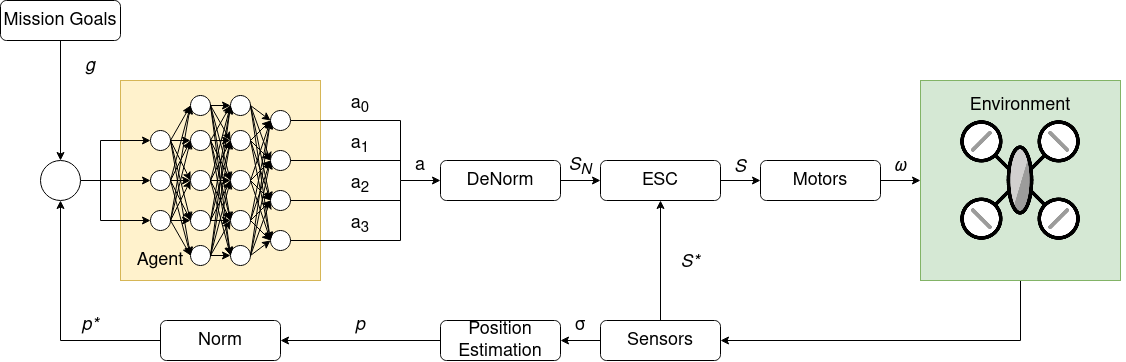
\includegraphics[width= 0.9 \linewidth]{figures/conceptAuto.png}
	\caption{Proposed Concept of autonomous flight control with the use of a intelligent agent implemented with the use of a NN. The output of the NN is denormalized in order to translate them to motor signals. With the use of the sensors and position estimation the input for the next control step are calculated.}
	\label{fig:conceptAuto}
\end{figure}

\newpage



\chapter{Implementation}
	The concept of implementation can be divided into the used packages (\emph{Stable Baselines3, Gym Pybullet Drones, ...}), the scripts, the environment classes and different support classes (\cref{fig:concept}).\\
Stable Baselines3 is used as implementation of the PPO algorithm (\cref{alg:ppo}) in order to achieve the tasks. Gym Pybullet Drones has already some environments and is the foundation of the simulation. It already provides a suitable step function and a well designed physics engine.\\
The scripts (\cref{sec:scripts} , lila) are used to either learn the agent on a given environment or evaluate it.\\
The environment classes(\cref{sec:env}, green) inherit from a \emph{Gym Environment} and models a MDP. By modelling this MDP precisely, it is defined what is learned later by the intelligent agent. It uses the wind class in order to model a harsh environment.
In addition, there are a couple of evaluation tools (\cref{sec:tools}, red), that supports the implemented classes.\\
\newline
The whole concept is implemented in Python3.x with the use of a \emph{conda environment}.

\begin{figure}[htp]
	\centering
	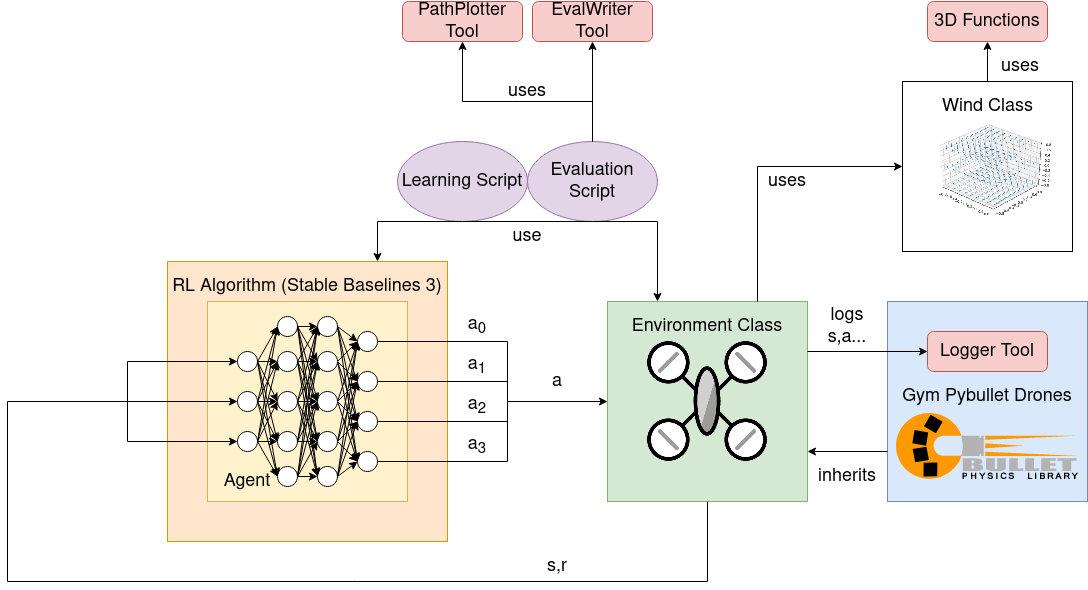
\includegraphics[width= \linewidth]{figures/concept.png}
	\caption{Concept of the implemented software: the different tools(red), scripts(violet) that are used in order to learn the intelligent Agent robust flight control with the use of RL.}
	\label{fig:concept}
\end{figure}
\newpage

\section{Environment Classes} \label{sec:env}



\subsection{WindSingleAgentAviary Environment Class}

\newpage

\subsubsection{Wind Class}

\newpage

\subsubsection{Modes}\label{sec:modes}

\newpage

\subsubsection{Observation Space \& State Space}
The state space $S$ defines the state vector of the drone in the environment and possesses a dimensionality of $23$. This state is only used inside the evironment and consists of the current position $x_p, y_p, z_p$ in each axis, the roll, pitch and yaw angles $\Theta_p, \phi_p, \psi_p$ as well as represented as quaterion $q$, the velocities $\dot{x_p}, \dot{y_p}, \dot{z_p}$, the angular velocities $dot{\Theta_p}, \dot{\phi_p}, \dot{\psi_p}$, the goal position $x_g, y_g, z_g$ and the last clipped action $a_t$. With the use of this drone state space the observations are calculated.\\
\newline
The observation space $\sigma$ is a subset of the state space $S$ with the dimensionality of 15. The observation space is implemented as a \emph{spaces box} of type \emph{float32} wich are mainly ranged within $[-1, 1]$ with the exception of the z coordinate of the position $z_p$ and goal $z_g$. Because there is floor defined as a plain at the height of $0$, which inherits a collision body, the drone is not able to reach a negative z coordinate. As a consequence, these are ranged to $[0,1]$.
\newline
\begin{align}
	\sigma_t &= (x_p,y_p,z_p, \Theta_p, \phi_p, \psi_p, \dot{x_p}, \dot{y_p}, \dot{z_p}, \dot{\Theta_p}, \dot{\phi_p}, \dot{\psi_p}, x_g, y_g, z_g) \label{eq:obs}
\end{align}
\newline
Each observation $\sigma_t$ consists of the current position $x_p, y_p, z_p$ in each axis, the roll, pitch and yaw angles $\Theta_p, \phi_p, \psi_p$, the velocities $\dot{x_p}, \dot{y_p}, \dot{z_p}$, the angular velocities $dot{\Theta_p}, \dot{\phi_p}, \dot{\psi_p}$ and the goal position $x_g, y_g, z_g$ (\cref{eq:obs}). These observations are given to the NN in order to approximate the optimal action $a$ that satefies the defined RL problem.\\
\newline
Like previously mentioned, all observations are ranged in order to prohibit inputs of different magnitude that could disrupt the learning process. This is done with the use of the method \emph{\_clipAndNormalizeState} which gets the current state $s_t$ and normalizes it to the defined range (\cref{eq:clipnorm}). First, it clips it to predifined values $v$ and then normalizes it by deviding with the matching predefined value $v_i, i\in[0,11]$. If wanted, a warning can be printed each time a state parameter has to be clipped. By clipping x and y to a value in $[-20,20]$ there is a predifed limit of maximal distance, in which there is a reasonable option to learn robust flight. Analogue the z component is clipped to $[-10,10]$, roll and pitch to $[-\pi, \pi]$, the translation velocities to $[-3, 3]$ in x,y and to $[-2,2]$ in z direction. 
\newline
\begin{align}
	\sigma_t \leftarrow clip(s_t) / v \label{eq:clipnorm}
\end{align}
\newline

\newpage

\subsubsection{Action Space}
The WindSingleAgentAviary Environment possesses three different type of action spaces, that are processed in different ways to the \emph{rpm (rotation per minute)} of the four motors (\cref{tab:act}). Nevertheless, all action types are continuous and are ranged in $[-1, 1]$.\\
\newline
\emph{one\_d\_rpm} is a one dimensional action space. The chosen action $a$ is processed to range of $\alpha$ about the \emph{hover\_rpm} to a 4-tupel of rpms. The hover\_rpm is defined as the rpm that corresponds to hovering (\cref{sec:hover}). The 4-tupel is then forwarded to the motors. As a consequence of this limitation, the drone can only perform hovering, rising and falling movements and can not influence its $x,y$ position or $\Theta, \phi, \psi$. Also, the translational speed $v_z$ is limited by the size of $\alpha$.\\
\newline
\emph{rpm} is a 4 dimensional action space. The actions are processed within a range of $\alpha$ about the hover\_rpm to a 4-tupel of rpms. The drone is not limited in any dimensionality, but the task increases in complexity. Due to \cref{form:quad}, \cref{form:quad2}, \cref{form:quad3}, \cref{form:quad4} even a small difference in rpms can lead to an unstable flight or even a crash, because the roll or pitch angle is to high. Also, all translational an rotational speeds are limited by the size of $\alpha$. Because of the higher complexity, it is expected, that the training takes noticeable more time.\\
\newline
\emph{vel} is a top level, 4-dimensional action space. The action consists of a velocity vector $v = (a_0, a_1, a_2)$ and its size $a_3$.  Since it is a top level action space, the actions are not corresponding directly to the rpms, but a pid controller (\cref{sec:pid}) is used in order to control the rpms. The basic pid controller is part of Gym Pybullet Drones \cite{panerati2021learning} and must be tuned for the used quadrocopter. It mainly receives the state $S$ of the drone, as well as the targeted velocity, which is calculated with the use of the actions. Therefore, $a_3$ is multiplicated with speed limit of the drone in order to derange the action. Also, the velocity vector $v$ is normalized to a length of $1$.\\
The drone is not limited in any dimensionality and the task is less complex then setting rpm directly. Stability of the flight is now mainly controlled by the pid controller, so it is bounded by the typical pid constraints in harsh environments and not adaptable.
\begin{table}
	\centering
	\caption{The different ActionTypes with the corresponding dimensionality of the action, its range and how it is processed.}\label{tab:act}
	\begin{tabular}{c|c|c|c}
		ActionType & dim & range & processing\\
		\hline
		\emph{one\_d\_rpm} & $|a| = 1$ & $a_i \in [-1, 1]$ & $rpm = (hover\_rpm \cdot (1 + \alpha \cdot  a)) \cdot (1, 1, 1, 1)$ \\
		\emph{rpm} & $|a| = 4$ & $a_i \in [-1, 1]$ & $rpm =  hover\_rpm \cdot (1 + \alpha \cdot  a)$ \\
		\emph{vel} & $|a| = 4$ & $a_i \in [-1,1]$ & $rpm = pid(S, vel= limit \cdot  |a_3| \cdot \frac{(a_0,a_1,a_2)}{|(a_0,a_1,a_2)|})$
	\end{tabular}
\end{table}


\newpage

\subsubsection{Reward}
\begin{figure}
	\centering
	\begin{subfigure}{0.3\linewidth}
		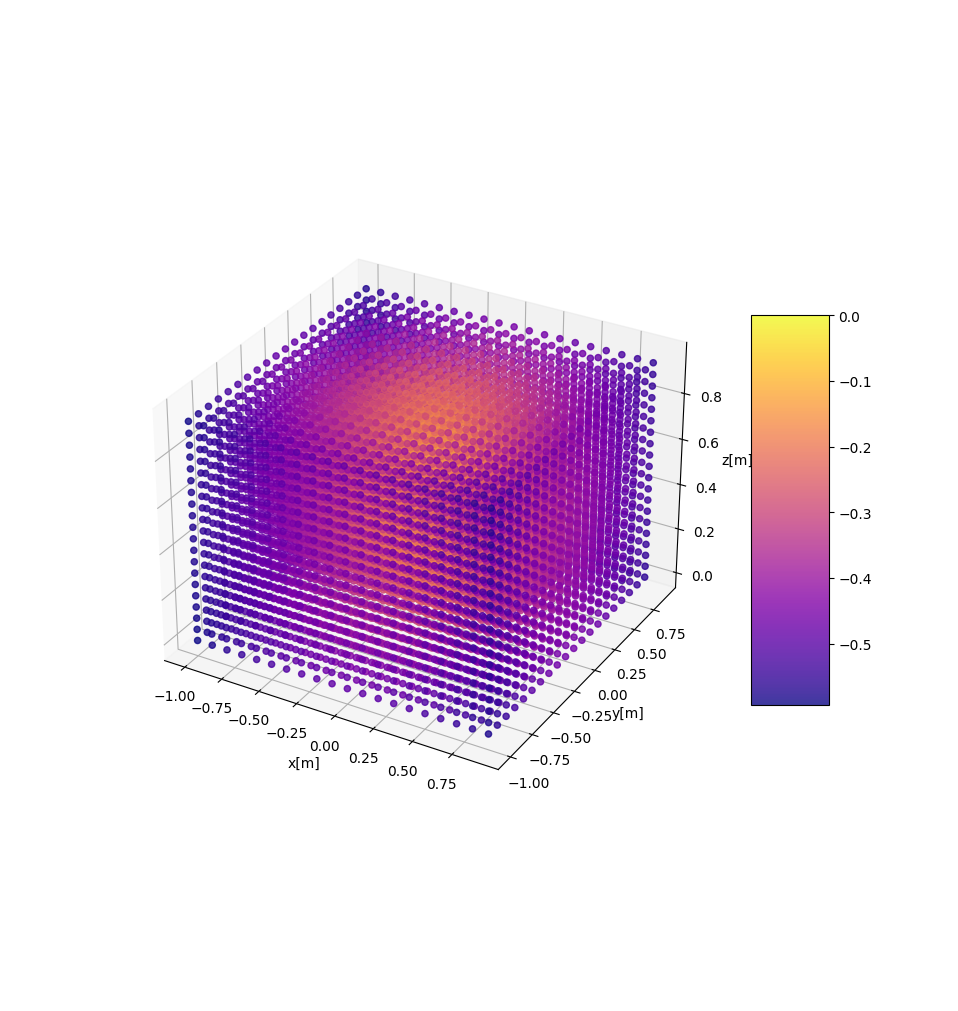
\includegraphics[width=\linewidth]{figures/rew3d.png}
		\caption{}
	\end{subfigure}
	\begin{subfigure}{0.3\linewidth}
		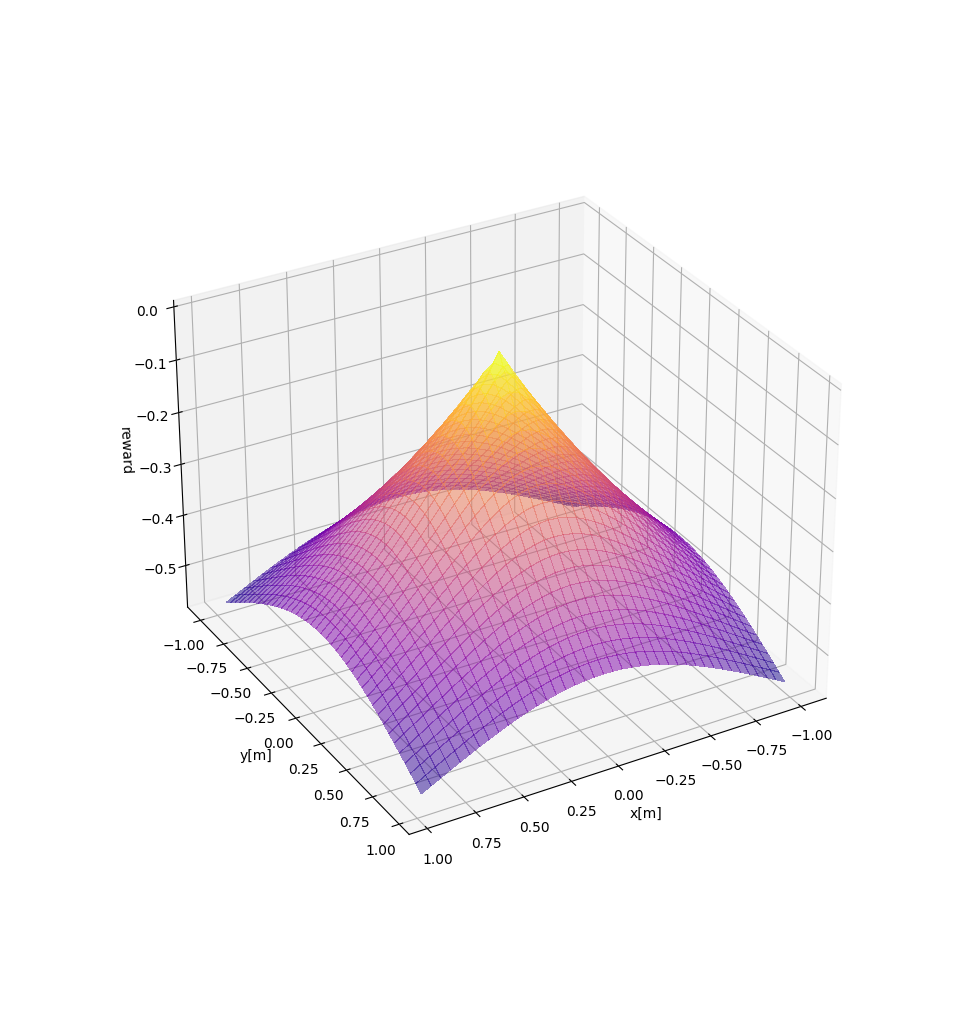
\includegraphics[width=\linewidth]{figures/rewXY.png}
		\caption{}
	\end{subfigure}
	\begin{subfigure}{0.3\linewidth}
		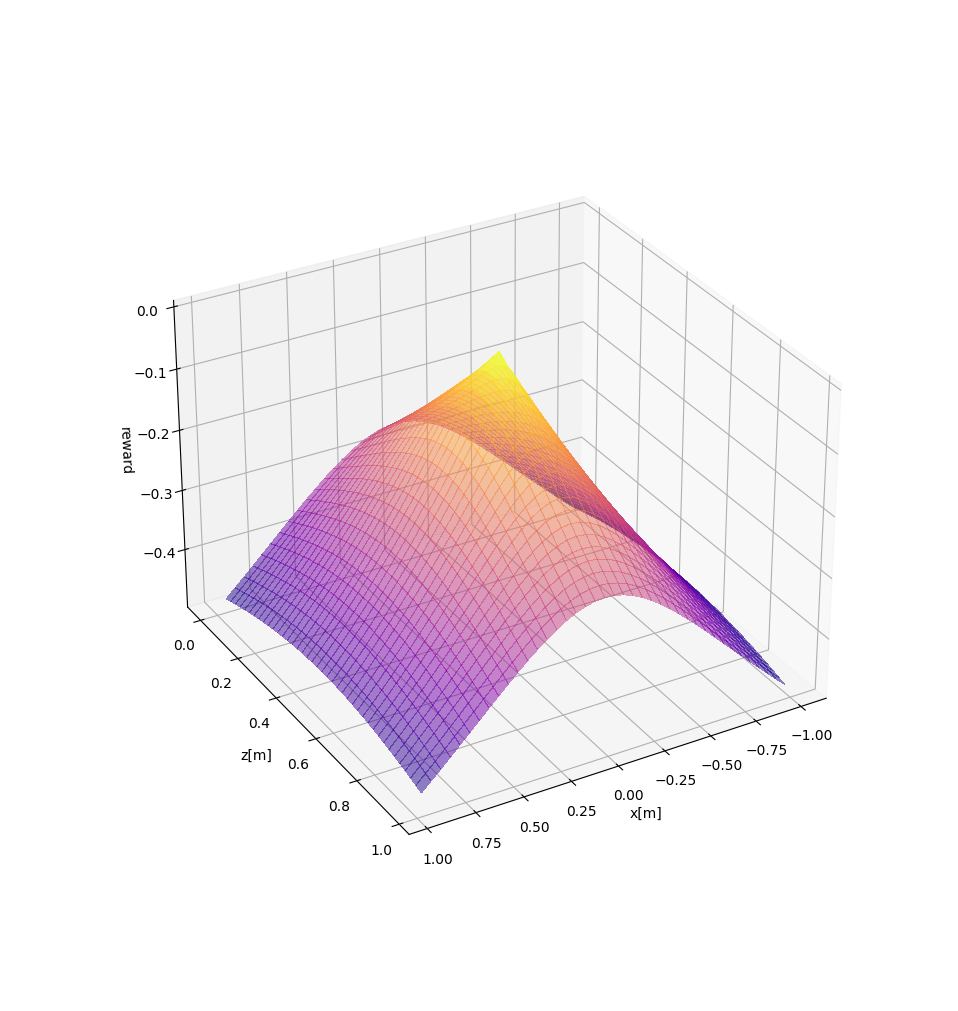
\includegraphics[width=\linewidth]{figures/rewXZ.png}
		\caption{}
	\end{subfigure}
	\caption{Visualization of the used reward function with the goal ($0,0,0.5$) and a colour scale for different positions in space.}
\end{figure}

\begin{align}
	r_t &= e^{-0.6 \cdot |goal - pos|} - 1 \label{eq:rew}
\end{align}

\newpage

\begin{figure}
	\centering
	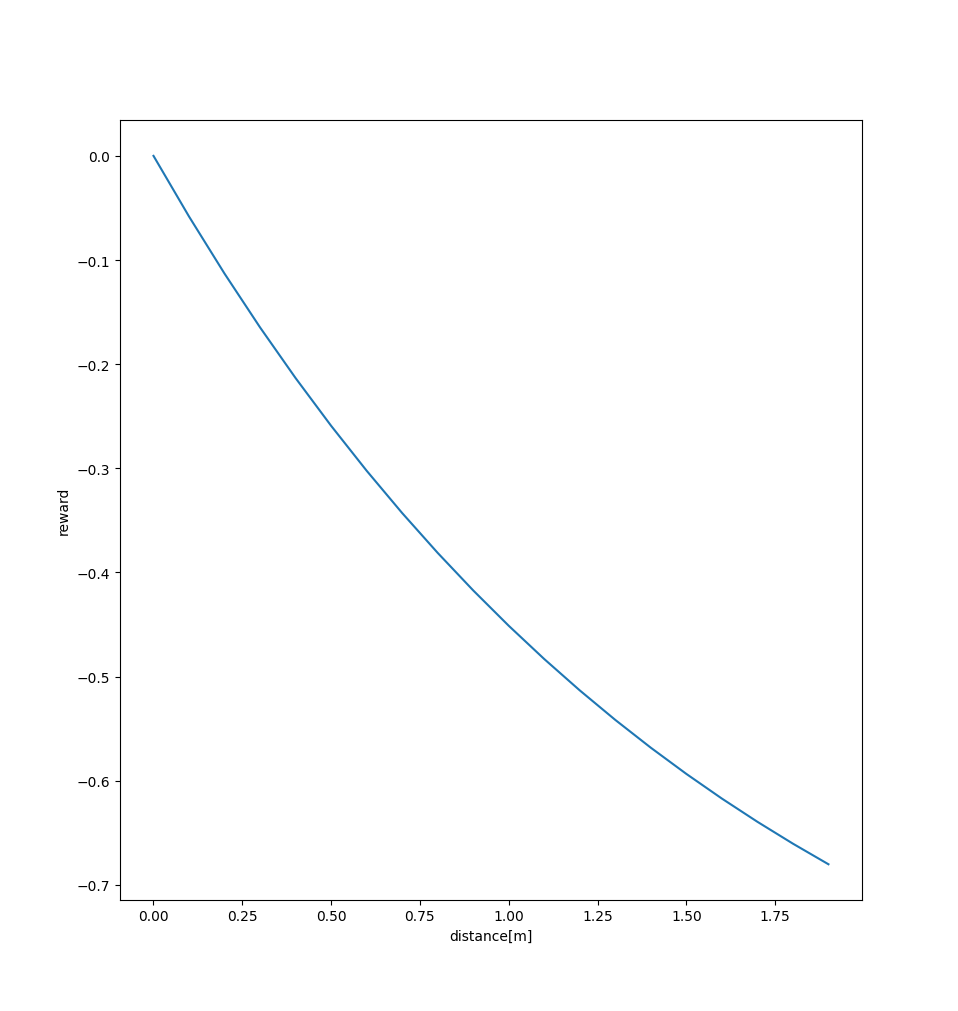
\includegraphics[width= 0.5\linewidth]{figures/reward.png}
	\caption{Visualization of the reward functions over the total distance[m]}
\end{figure}

\subsubsection{Constraints}
\begin{align}
	z_{p_t} \leq z_{min} \land \frac{t}{f} \geq 0.1 \to r_t = e^{-0.6 \cdot |goal - pos|} - 1 -200 \land done
\end{align}

\newpage

\subsubsection{Optimal Rewards}
Based on the modes (\cref{sec:modes}) different optimal rewards can be defined, that are helpful in order to determine how good the learned desicion making is.\\
\newline
\emph{Mode 0} is due to its fixed goal position $g$ rather easy to define:
\begin{align}
R_{opt} &= \sum_{t=0}^{f \cdot episode\_len} r_t \label{eq:oprew}\\
d_0 &= 0.5\\
d_{t+1} &= d_t - |v_{opt}| \cdot f \label{eq:dt1}\\ 
r_{t} &= e^{-0.6 \cdot (d_{t+1} )} - 1 \label{eq:rew2}
\end{align}
The distance at start $d_0$ is always 0.5. An optimal decision of the agent corresponds to an optimal velocity vector $v_{opt}$ that minimizes the distance to the goal with the given bounds of the maximum speed at the $\alpha$ of the action processing. The reward (\cref{eq:rew}) can then be reduced to \cref{eq:rew2} for every control step and summed up to the total optimal reward $R_{opt}$ (\cref{eq:oprew}).\\
\newline
Since \emph{mode 1} does not posess a fixed goal position, only a expected optimal reward $\mathbb{E}(R_{opt})$ can be defined. Therefore, an expected starting distance $\mathbb{E}(d_0)$ has to be used:
\begin{align}
	\mathbb{E}(d_0) &= \sqrt{\mathbb{E}(d_x)^2 + \mathbb{E}(d_y)^2 + \mathbb{E}(d_z)^2} \\
	\mathbb{E}(d_i) &= \int_{b_{min}}^{b_{max}} |i| di \\
	&= 
	\left\{
	\begin{array}{ll}
		 \int_{b_{min}}^{b_{max}} i di & \mbox{if } 0 \leq b_{min} \leq b_{max} \\
		 \int_{b_{min}}^{b_{max}} -i di & \mbox{if } b_{min} \leq b_{max} \leq 0\\
		\int_{b_{min}}^{0} -i di + \int_{0}^{b_{max}} i di  & \mbox{if } b_{min} \leq 0 \leq b_{max}
	\end{array}
	\right. \\
	&=
	\left\{
	\begin{array}{ll}
		\frac{1}{2} \cdot (b_{max}^2 - b_{min}^2) \enspace \enspace \enspace \enspace  & \mbox{if } 0 \leq b_{min} \leq b_{max} \\
		\frac{1}{2} \cdot (b_{min}^2 - b_{max}^2)  & \mbox{if } b_{min} \leq b_{max} \leq 0\\
		\frac{1}{2} \cdot (b_{min}^2 + b_{max}^2) & \mbox{if } b_{min} \leq 0 \leq b_{max}
	\end{array}
	\right.
	\label{eq:expd}
	%\int_{b_{min}}^{0} -i di + \int_{0}^{b_{max}} i di = [-\frac{1}{2}i^2]_{b_{min}}^{0} + [\frac{1}{2}i^2]_0^{b_{max}}\\
	%&= -(- \frac{1}{2} b_{min}^2) + \frac{1}{2} b_{max}^2 = \frac{1}{2} \cdot (b_{min}^2 + b_{max}^2)
\end{align}
The expected distance in each axis $\mathbb{E}(d_i)$ mostly depend on the defined bounds of the goal.\\
\newline
All other modes possess a wind class that trys to disrupt the agent. Since there are random wind fields and the corresponding force is not noramlly distributed, the optimal reward can just estimated downwords. Therefore, the used maximum wind force $W$ is used in order to approximate the maximum of disruptive distance and use it in order to update \cref{eq:dt1}.
\begin{align}
	d_{t+1} &= d_t - | v_{opt} | \cdot f + \frac{W}{m} \cdot f
\end{align}
\newpage

\subsection{WindSingleAgentPathfollowingAviary Environment Class}


\newpage

%%%%%%%%%%%%%%%%%%%%%%%%%%%%%%%%%%%%%%%%%%%%%
\section{Scripts \& Evaluation Tools} \label{sec:scripts}


%\subsection{TestInstall Script}

\subsection{Learning Script}
\begin{algorithm}
	\caption{Learning Script}
	\label{alg:learn}
	 Parse the arguments to the Script
	 
	 Check the parsed arguments on contradiction and raise ParsingError if needed
	 
	 Create training environment with the parsed parameters
	 
	 Define the size of the actor and critic policy network
	 
	 Create or load the model based on the parsed load argument
	 
	 Create evaluation environment with the parsed parameters
	 
	 Define evaluation callbacks
	 
	 Learn the model with the parsed amount of time steps
	 
	 Save the model with the parsed preferred name
	 
	 
\end{algorithm}

\newpage

\subsection{Evaluation Script}
\begin{algorithm}
	\caption{Evaluation Script}
	\label{alg:eval}
	Parse the arguments to the Script
	
	Check the parsed arguments on contradiction and raise ParsingError if needed
	
	Create evaluation environment with the parsed parameters
	
	Define the size of the actor and critic policy network
	
	Load the model
	
	Instantiate an EvalWriter and evaluate the model
	
	\If{gui parameter was parsed as true}{
		Instantiate a test environement, logger and a pathplotter
		
		Reset environment and safe an observation $\sigma$
		
		
		Safe current time $t$
		
		\Repeat{done or time is over}{
		Get action $a$ and the observation $\sigma$
		
		Execute a step in the test environment and receive an observation $\sigma$, a reward $r$, a done value and a info
		
		Add current pose to pathplotter
		
		Log current drone state
		
		Sync simulation time $t_sim$ to the real time $t$}
		Close test environment, show the plotted path and the values.
	}


\end{algorithm}

\newpage

%%%%%%%%%%%%%%%%%%%%%%%%%%%%%%%%%%%%%%%%%%%%%%
\subsection{Evaluation Tools} \label{sec:tools}

\subsubsection{EvalWriter Class}

\newpage

\subsubsection{PathPlotter Class}


%\chapter{Evaluation Tools}
%	\input{content/evalsetup.tex}

\chapter{Evaluation}
	\section{Drone Model}

\newpage

\section{Setup}

\newpage

\section{Metric}

\newpage

\section{Results}

\chapter{Conclusion \& Future Work}
	\section{Of Migrating to a real Drone}

\newpage

\section{Of Hovering \& Pathfollowing}

\newpage

\section{Of Improvents in Self-Pased Curriculm Learning}

\newpage

\section{Of Policy Ensembles for Sub-Problem-Solving}


%\chapter{Appendix}
	\chapter*{Appendix A - Algorithms for Evaluation}
\addcontentsline{toc}{chapter}{Appendix A}

\begin{algorithm}
	\caption{Update Algorithm of EvalWriter}
	\label{alg:upd}
	Get current $dist$ and $t_{sim}$ from environment $\epsilon$ and save it
	
	\If{$e = 1$}{
		Add pose of the drone from $\epsilon$ to pathplotter
		}
		
	\If{$t_{sim} = \frac{T}{2}$}{
		Save current $dist$ to matching set of distances
		}
		
	\If{$t_{sim} = T$}{
		Save current $dist$ to matching set of distances
	}
	
	\If{episode already reached goal and overshoot}{
		Save current $dist$ to overshoot set
	}
	
	Check if the episode succeeded in this time step
\end{algorithm}

\begin{algorithm}
	\caption{Evaluation Algorithm of EvalWriter}
	\label{alg:evalwriter}
	\KwIn{policy $\pi$}
	\KwOut{tupel ($\mu_r, \sigma_r$)}
	
	Get mean return $\mu_r$ and the std of the return $\sigma_r$ from $evaluate\_policy (\pi , \epsilon, e)$
	
	reset $\epsilon$ and receive $\daleth_t$
	
	\For{$j=0 \to \gimel$}{
		\Repeat{$done$}{
			Get action $a$ from $\pi$ with input $\daleth_t$
			
			Step $\epsilon$ and get the new observation $\daleth_t$, reward $r_t$, done signal $d$  and info
			
			Update EvalWriter
			
			\If{$d$}{
				Reset $\epsilon$
				}
		}
		\If{not $j = \gimel$}{
			Use Housekeeping of the EvalWriter class
			}
	}
	Close EvalWriter and $\epsilon$.
	
	\Return ($\mu_r, \sigma_r$)
	
\end{algorithm} 

\newpage

\chapter*{Appendix B - Flight \& Distance Data}
\addcontentsline{toc}{chapter}{Appendix B}

\begin{figure}[htp]
	\centering
	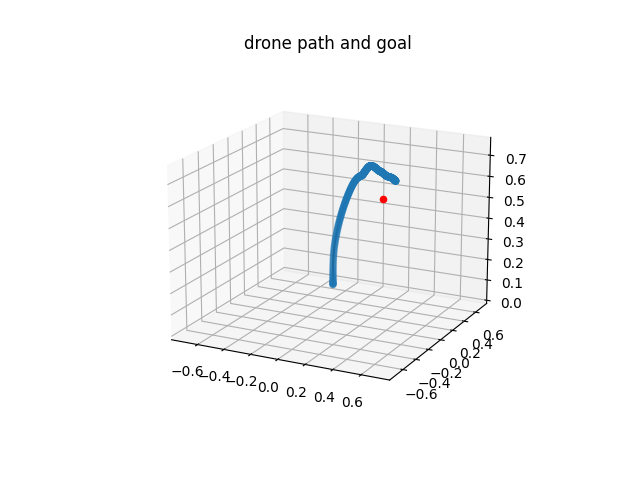
\includegraphics[width=0.6\linewidth]{figures/exampleflight1.png}
	\caption{Example of a flight with SAC policy on mode 2 within a radius of $0.5m$}
	\label{fig:flight0}
\end{figure}

\begin{figure}[htp]
	\centering
	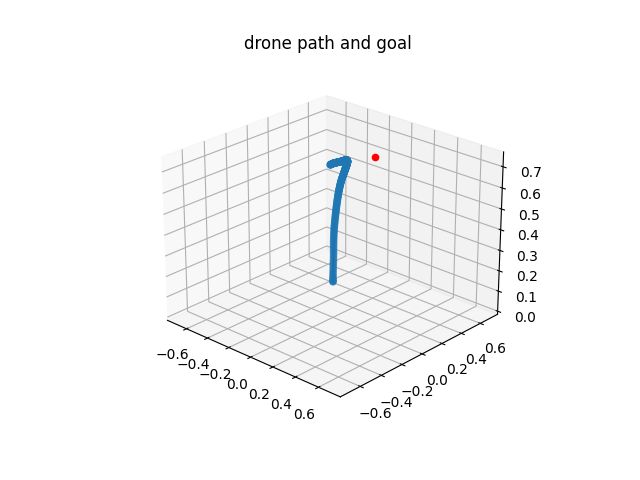
\includegraphics[width=0.6\linewidth]{figures/flight2.png}
	\caption{Example of a flight with SAC policy derived from LCL with $\delta = 0.4$ on mode 2 within a radius of $0.5m$}
	\label{fig:flight1}
\end{figure}

\begin{figure}[htp]
	\centering
	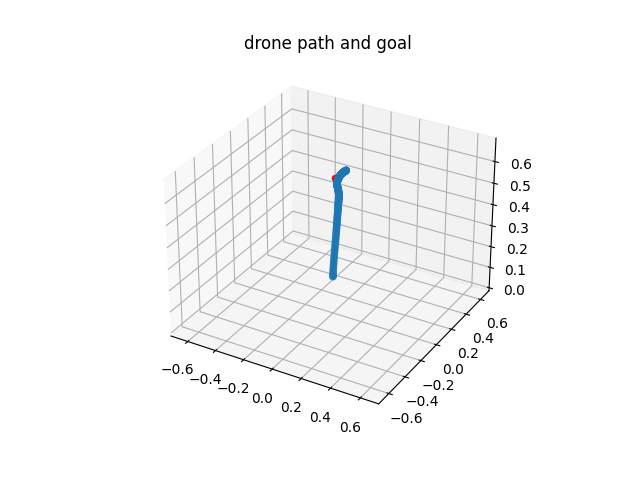
\includegraphics[width=0.6\linewidth]{figures/flight3.png}
	\caption{Example of a flight with SAC policy derived from LCL with $\delta = 0.2$ on mode 2 within a radius of $0.5m$}
	\label{fig:flight2}
\end{figure}

\begin{figure}[htp]
	\centering
	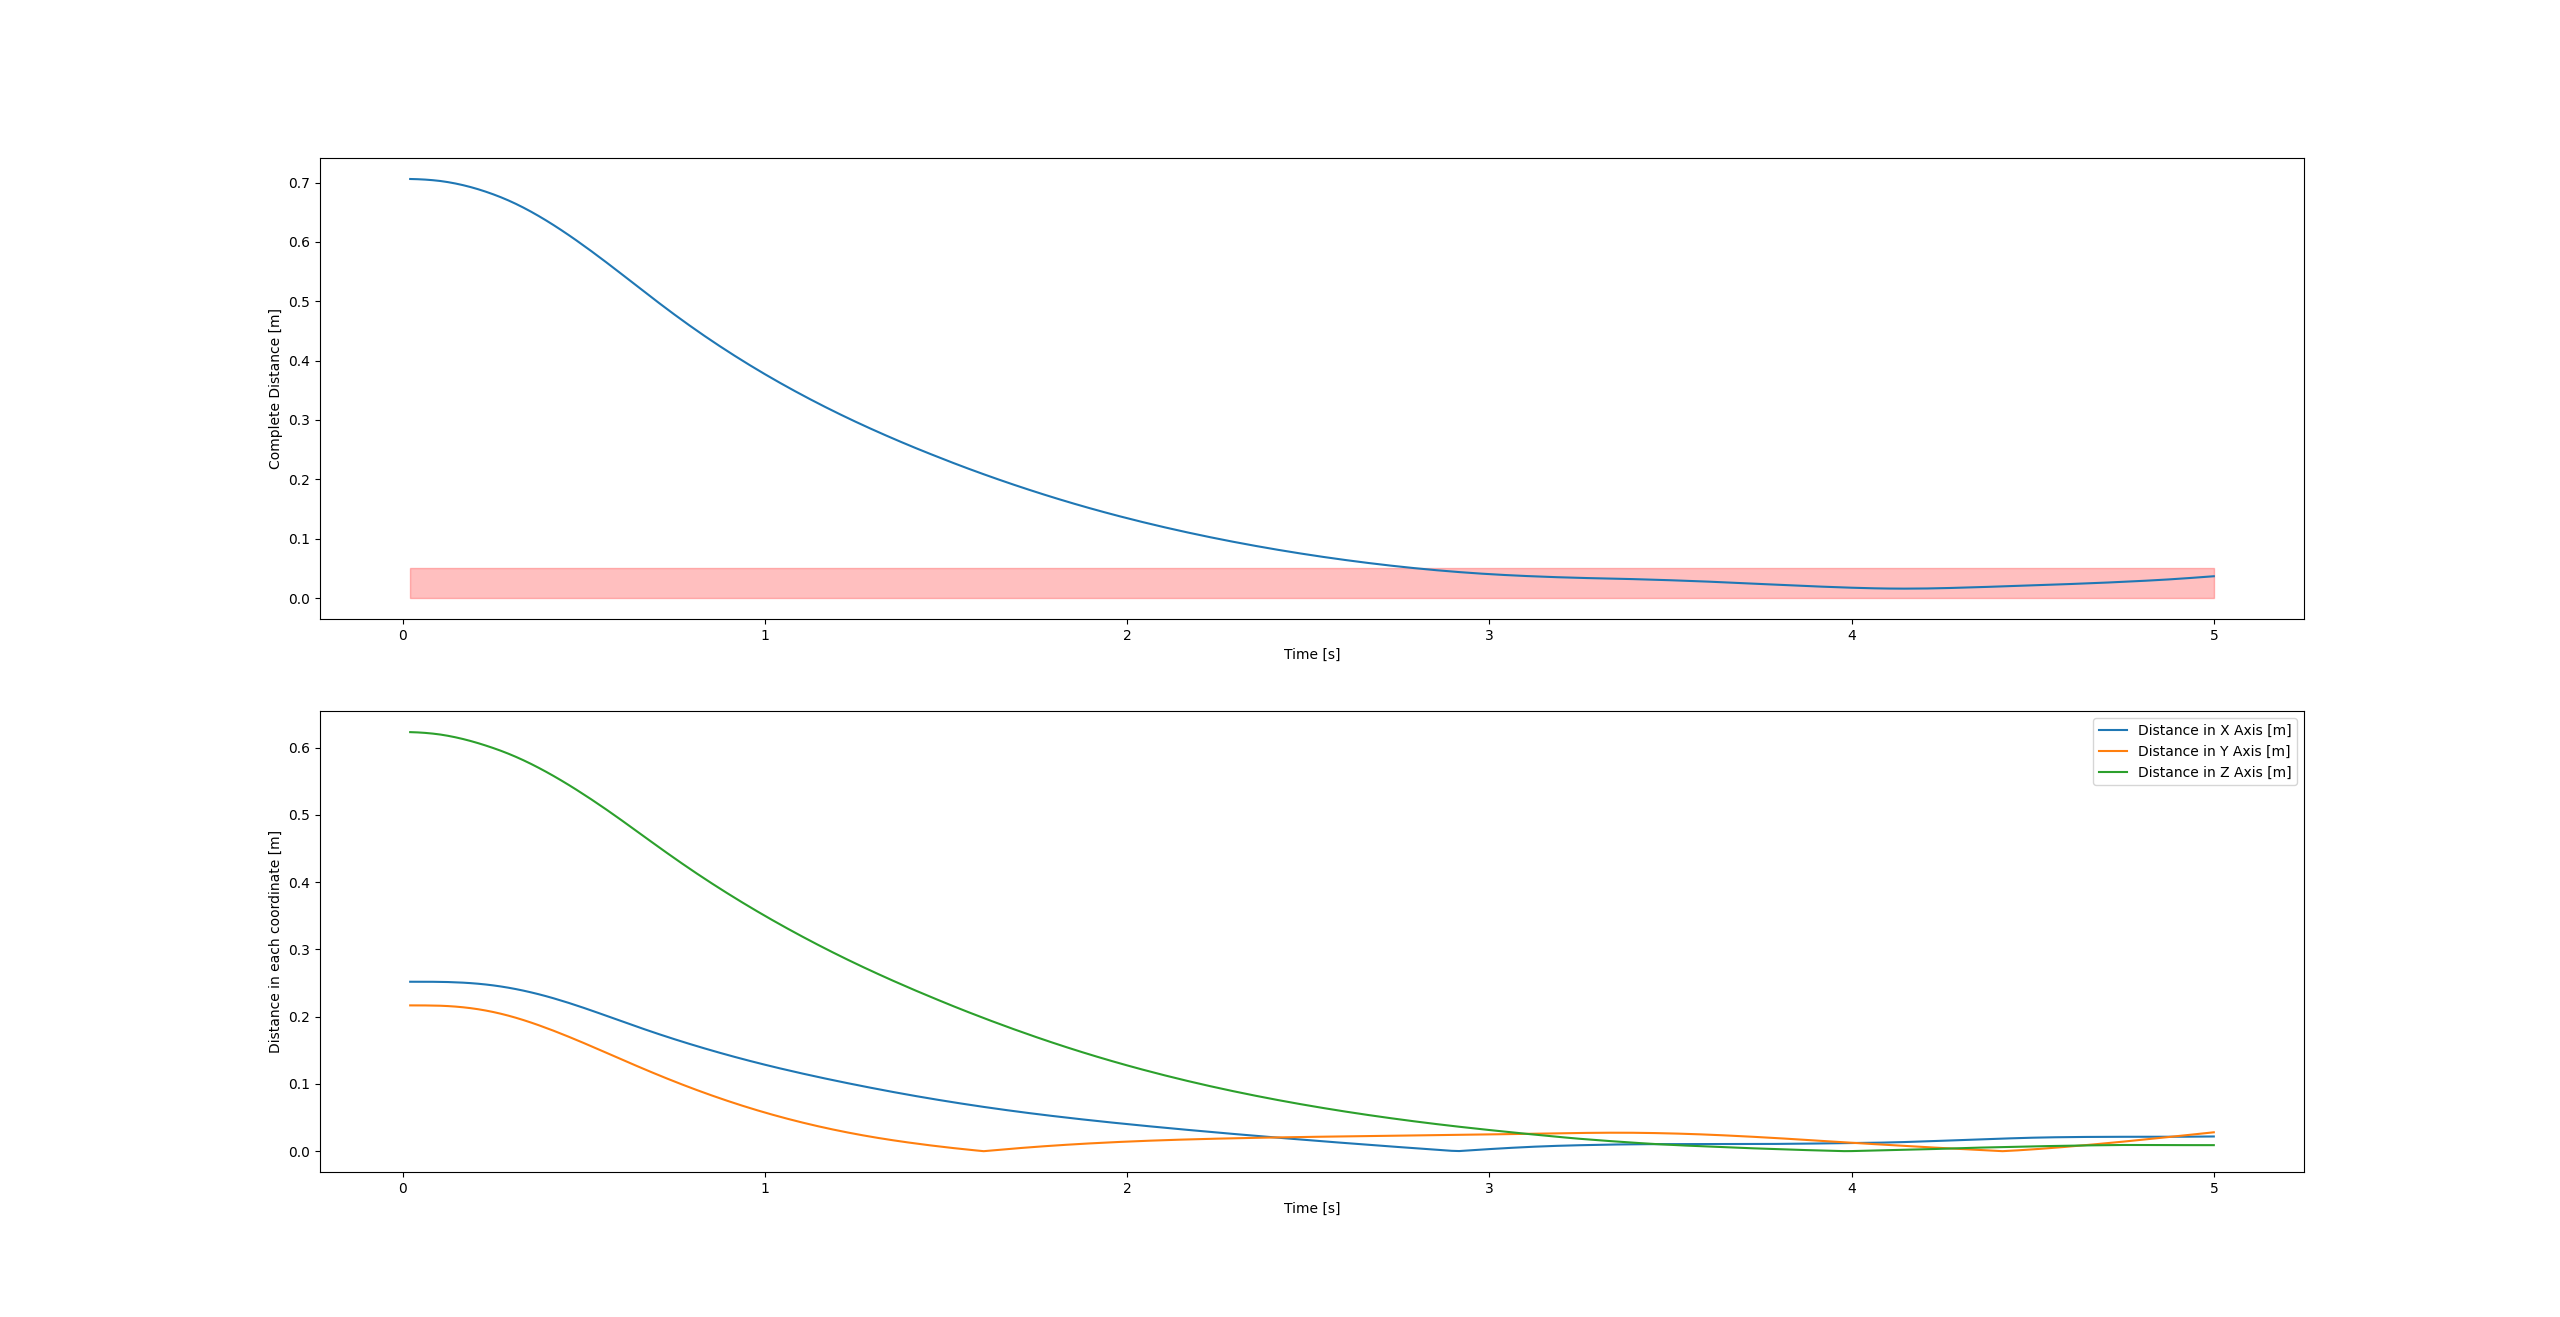
\includegraphics[width=\linewidth]{figures/flight4dist.png}
	\caption{Example of distances with SAC policy on mode 2 within a radius of $0.5m$}
	\label{fig:flight3}
\end{figure}

\begin{figure}[htp]
	\centering
	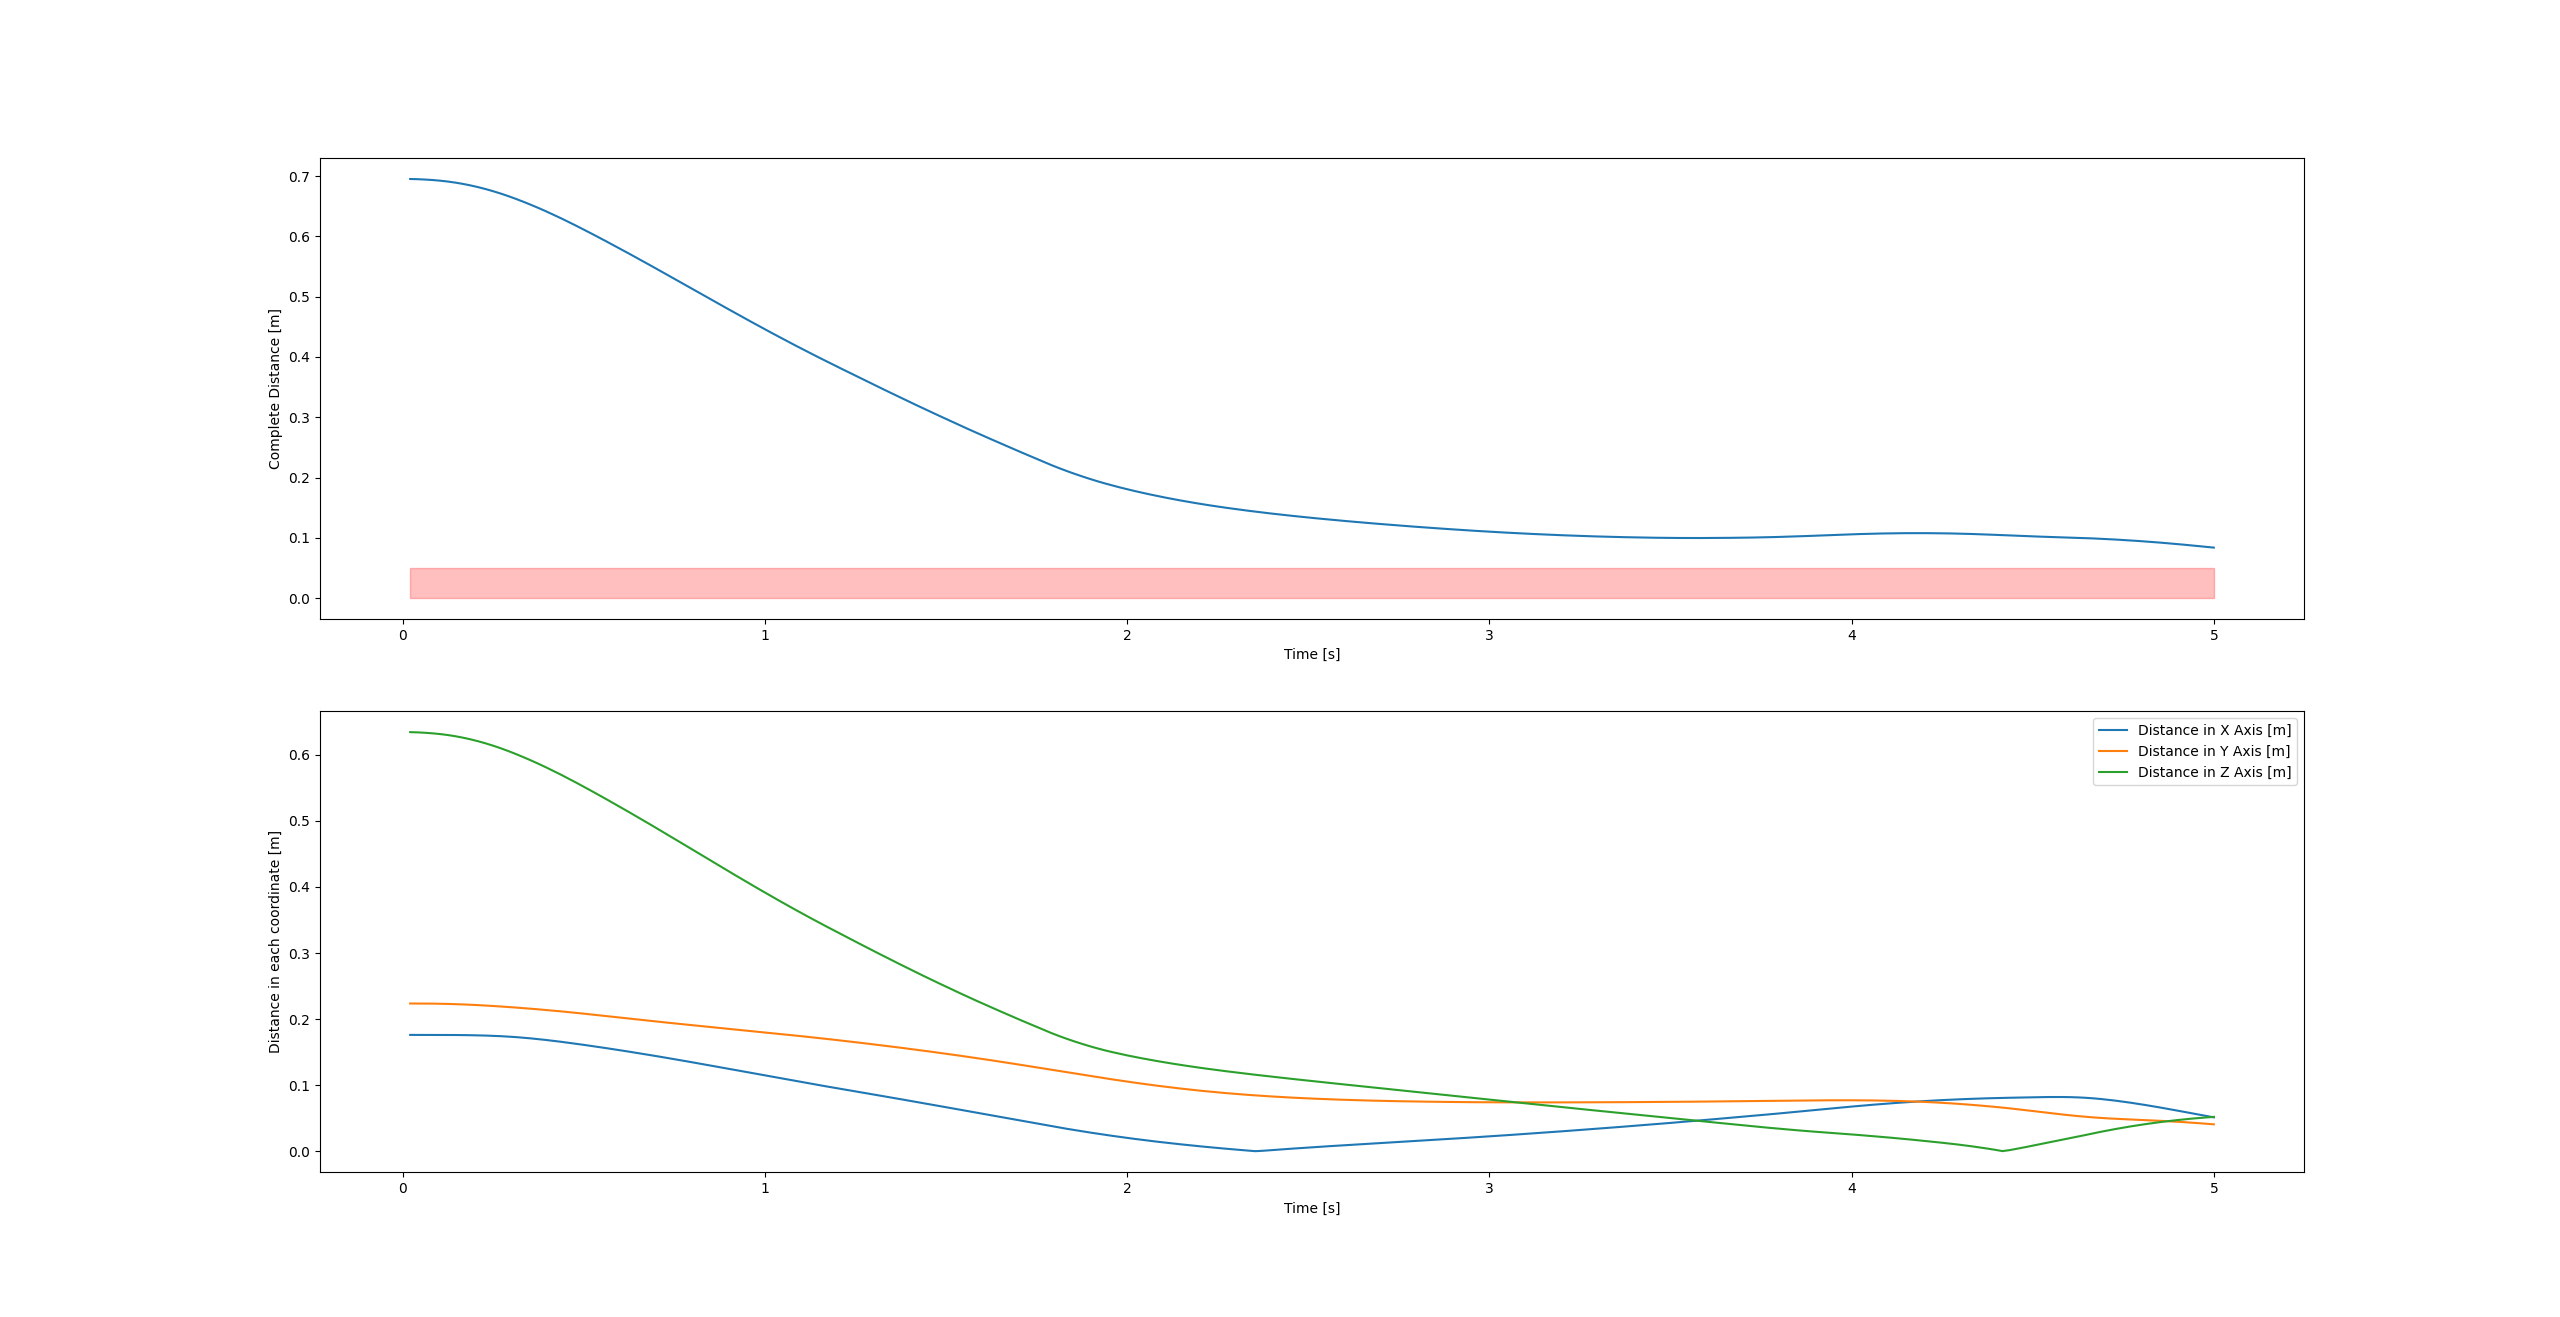
\includegraphics[width=\linewidth]{figures/flight5dist.png}
	\caption{Example of distances with SAC policy derived from LCL with $\delta = 0.4$ on mode 2 within a radius of $0.5m$}
	\label{fig:flight4}
\end{figure}

\begin{figure}[htp]
	\centering
	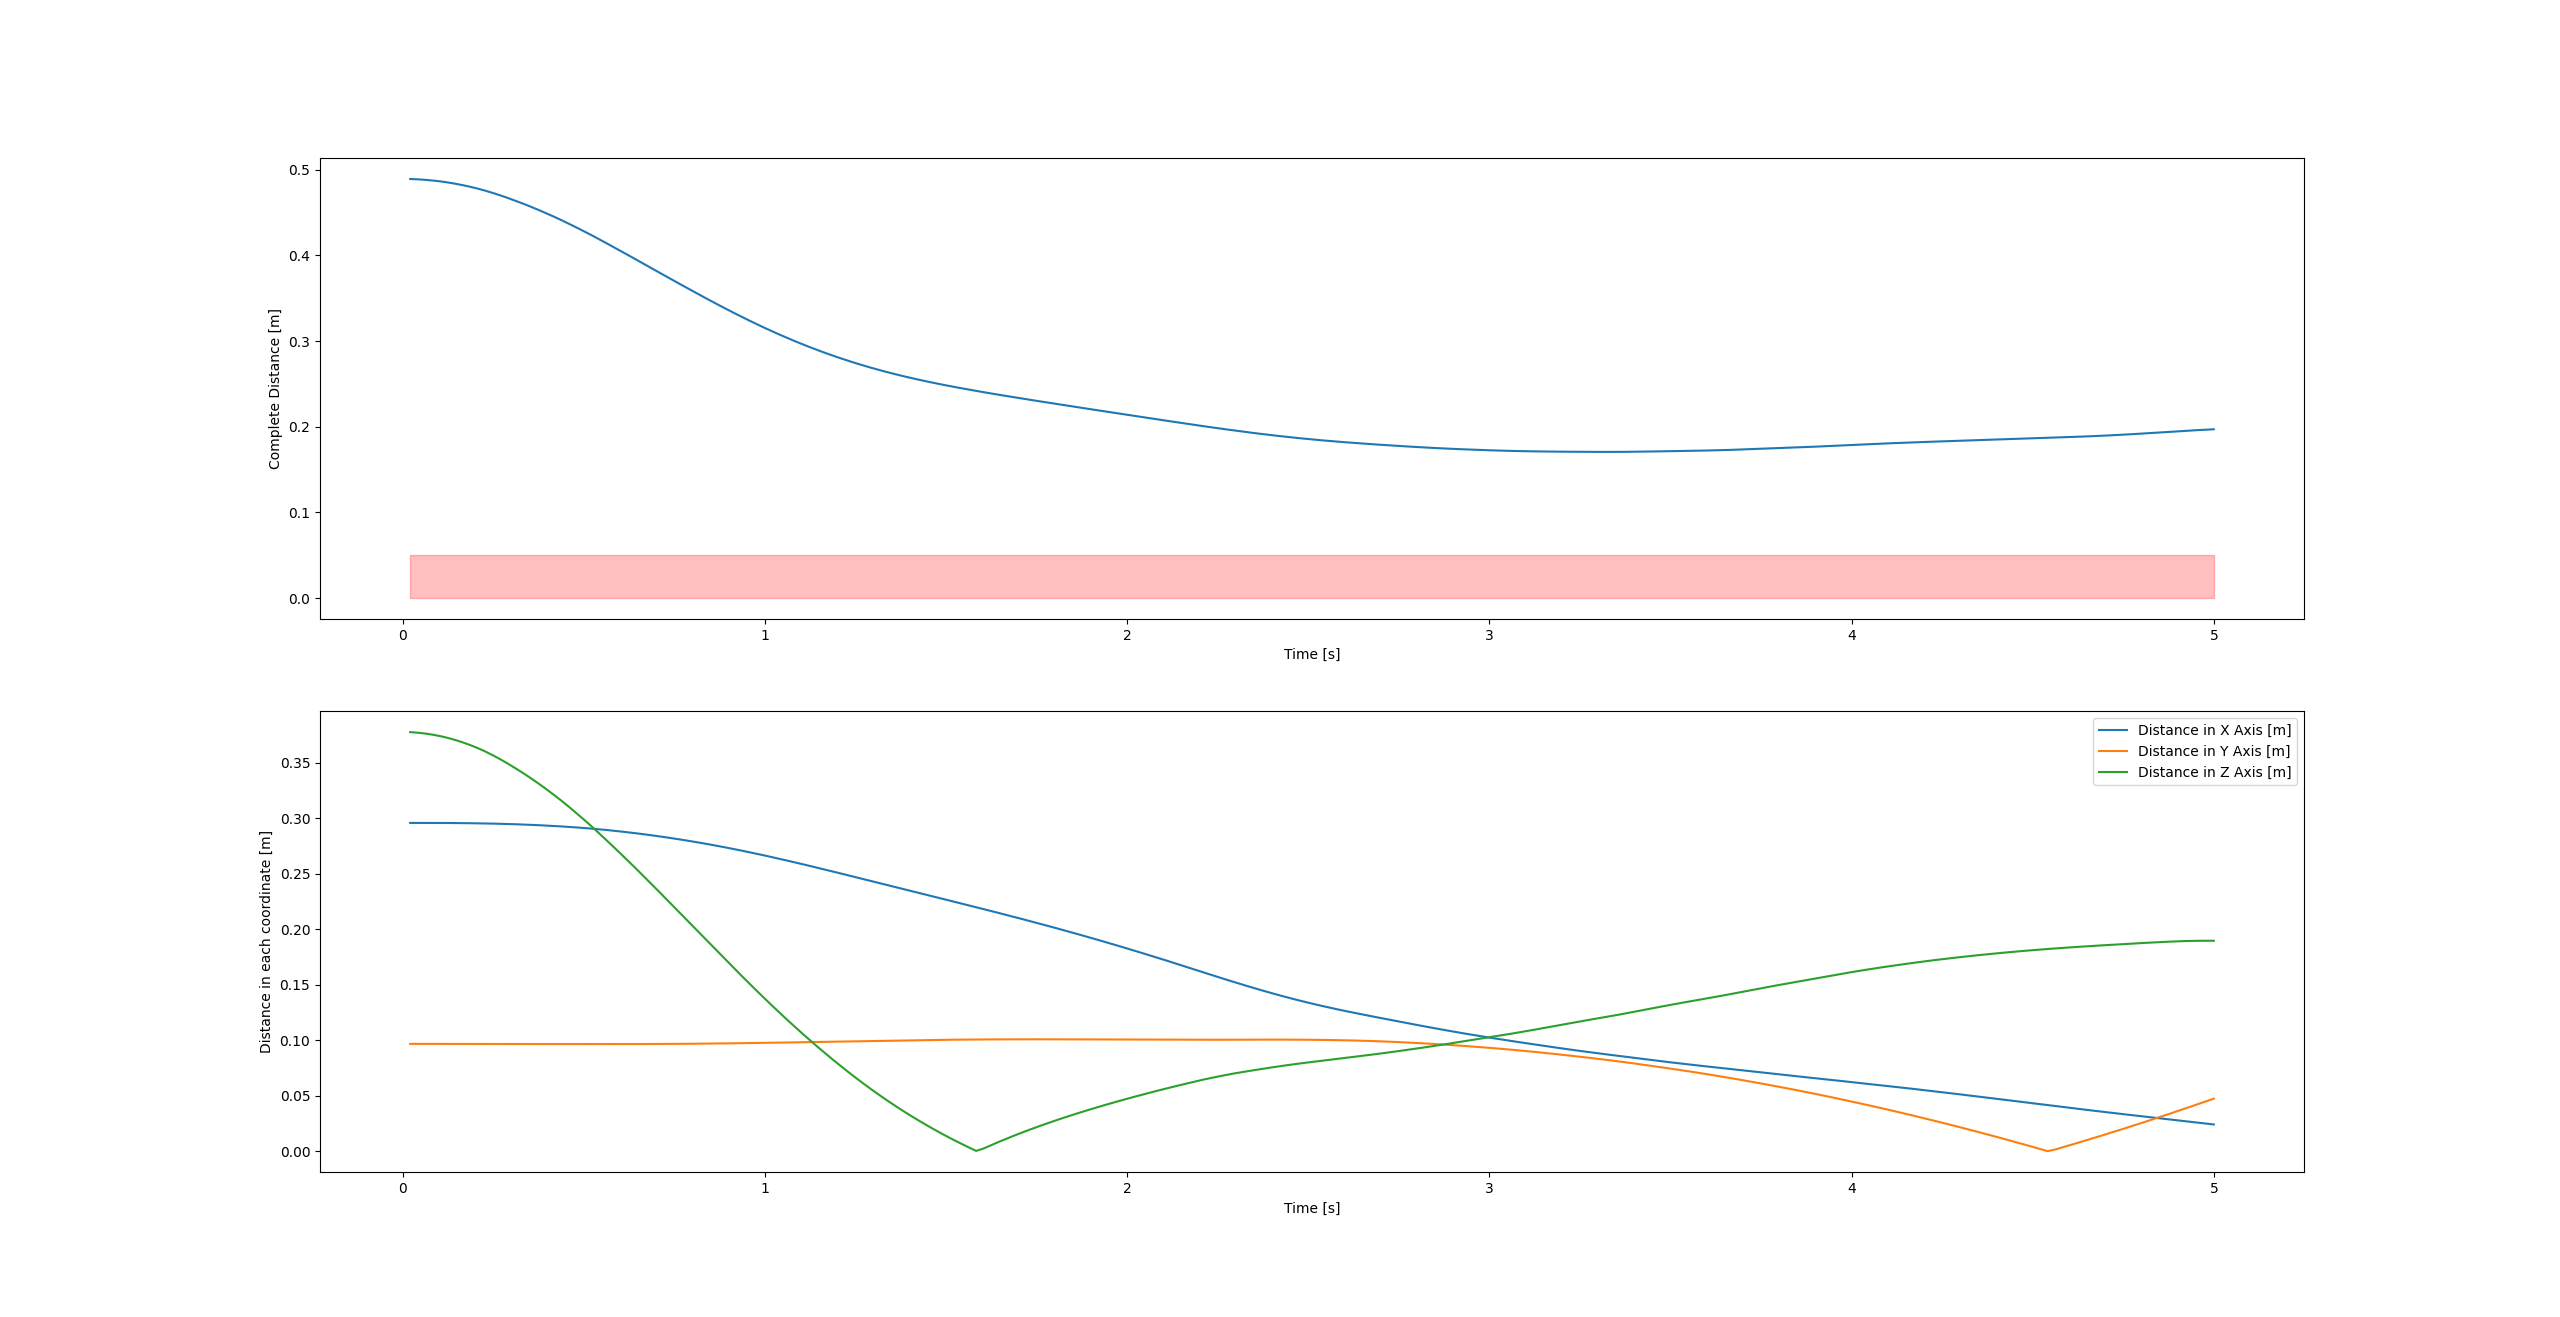
\includegraphics[width=\linewidth]{figures/flight6dist.png}
	\caption{Example of a distances with SAC policy derived from LCL with $\delta = 0.2$ on mode 2 within a radius of $0.5m$}
	\label{fig:flight5}
\end{figure}

\begin{figure}
	\centering
	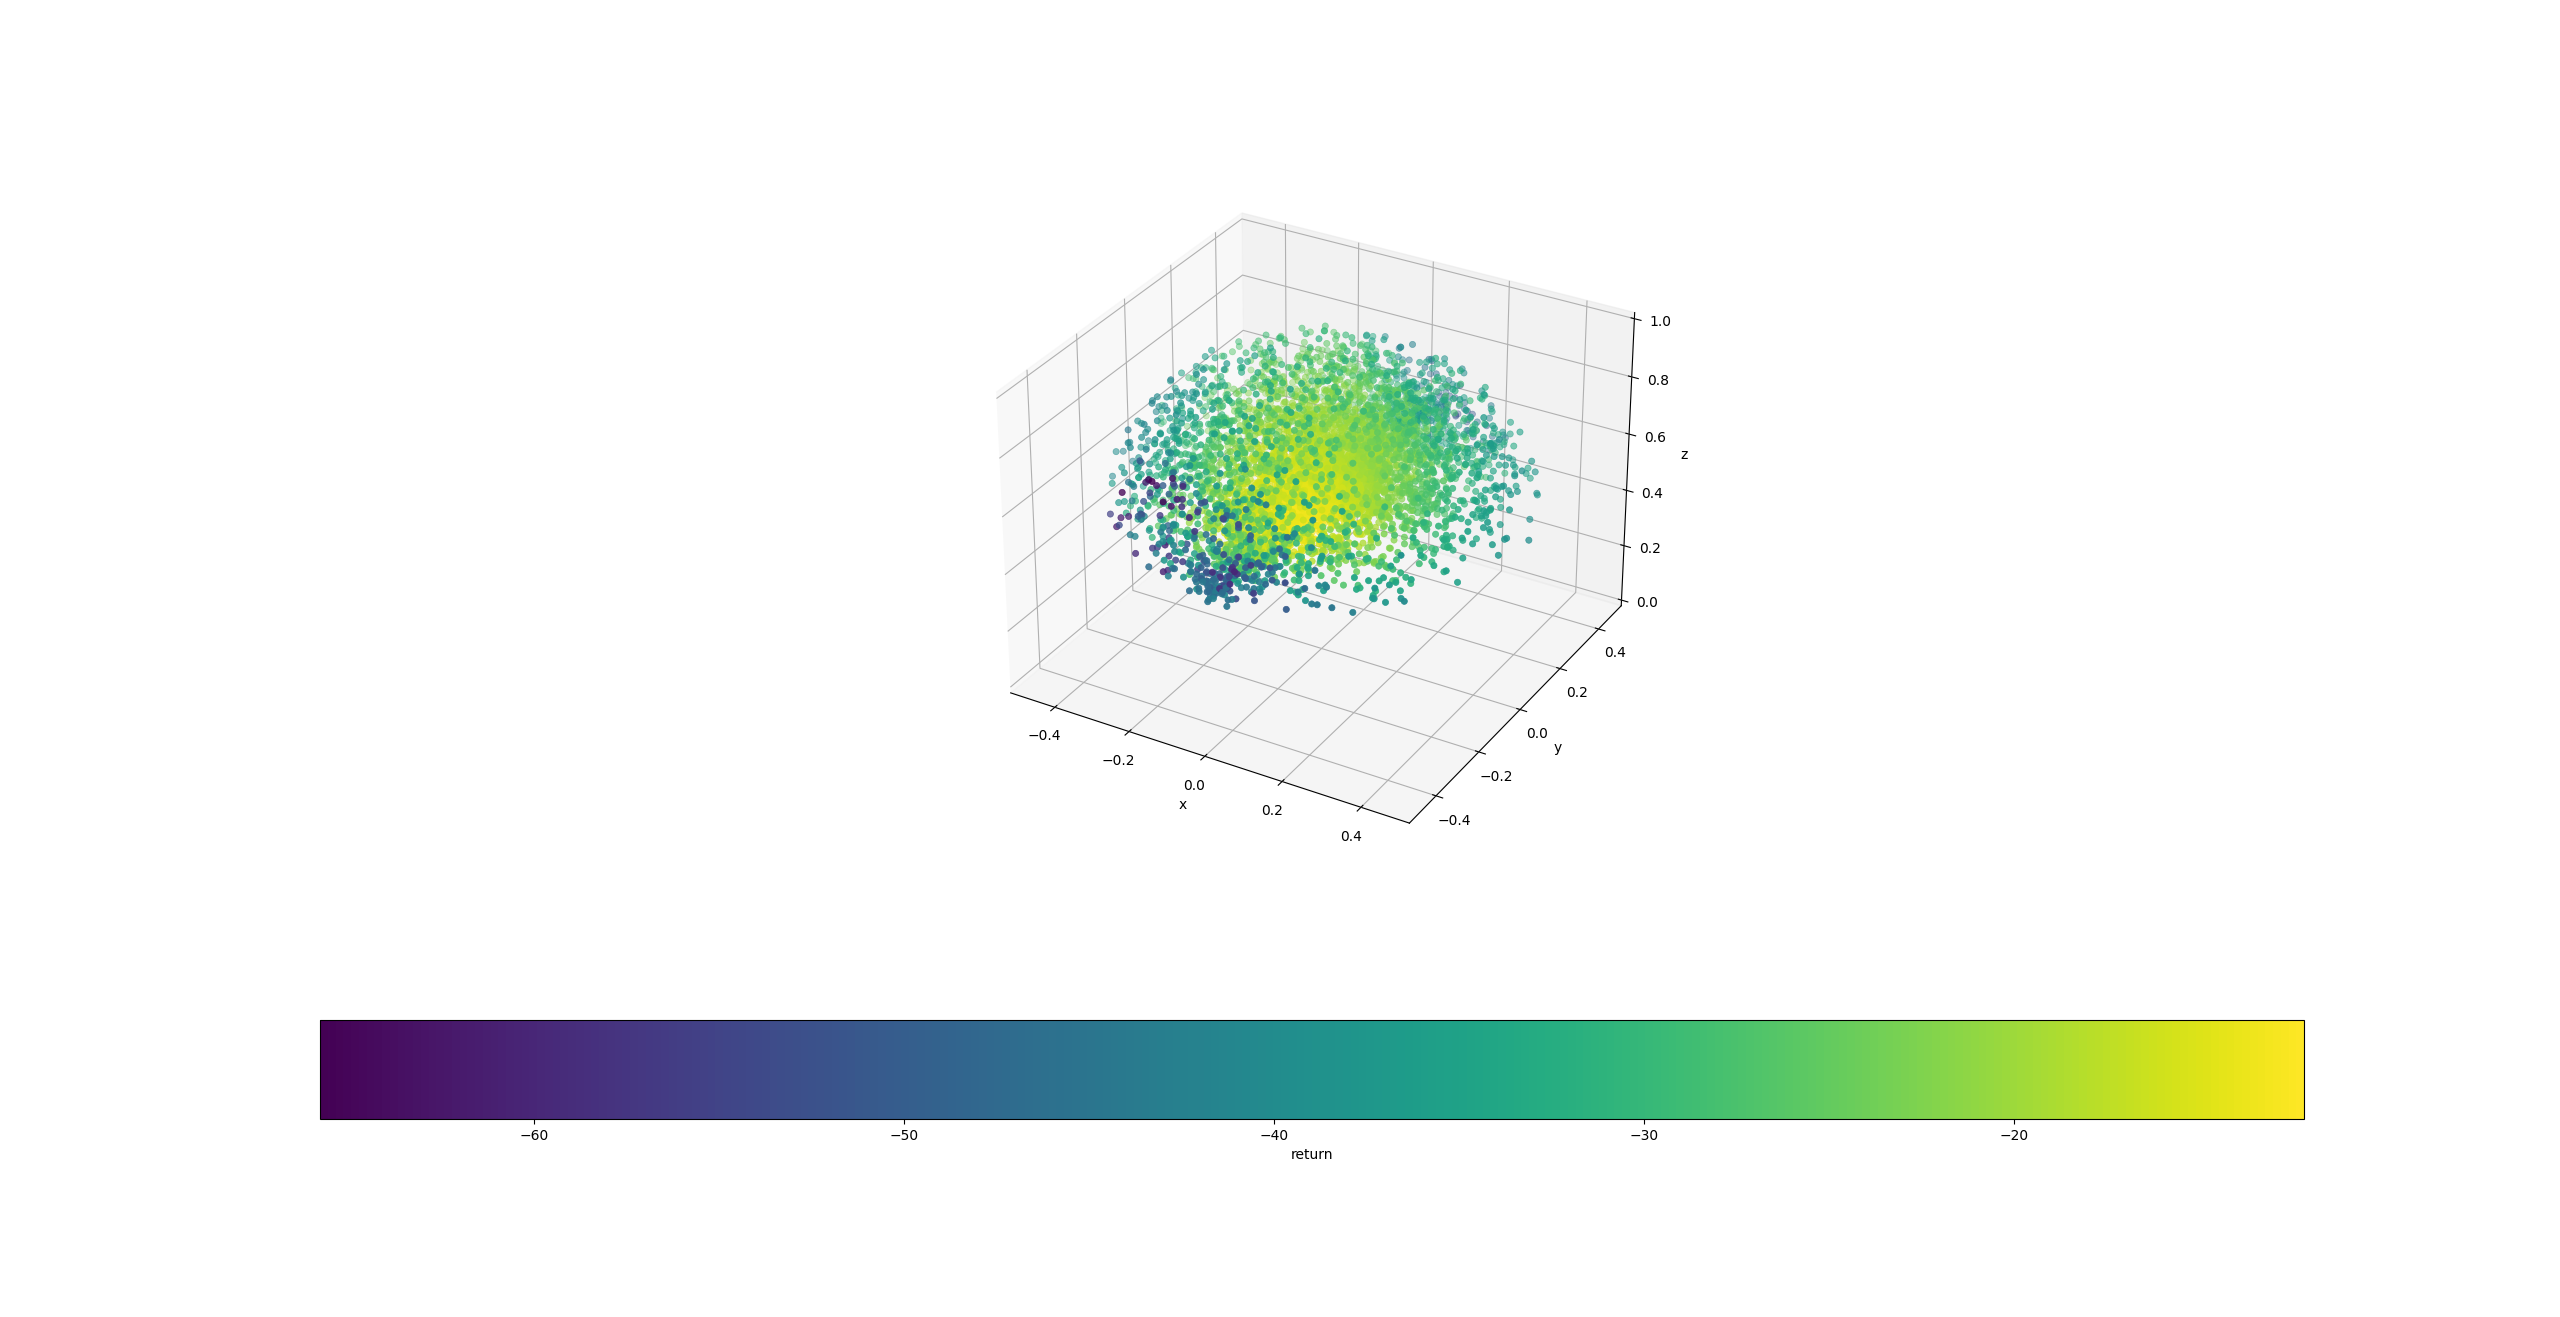
\includegraphics[width=\linewidth]{figures/potentialplot1.png}
	\caption{Expected Return of SAC policy for $7500$ random goals inside the 
	goal ball with a radius of $0.5m$}
	\label{fig:pot1}
\end{figure}

\begin{figure}
	\centering
	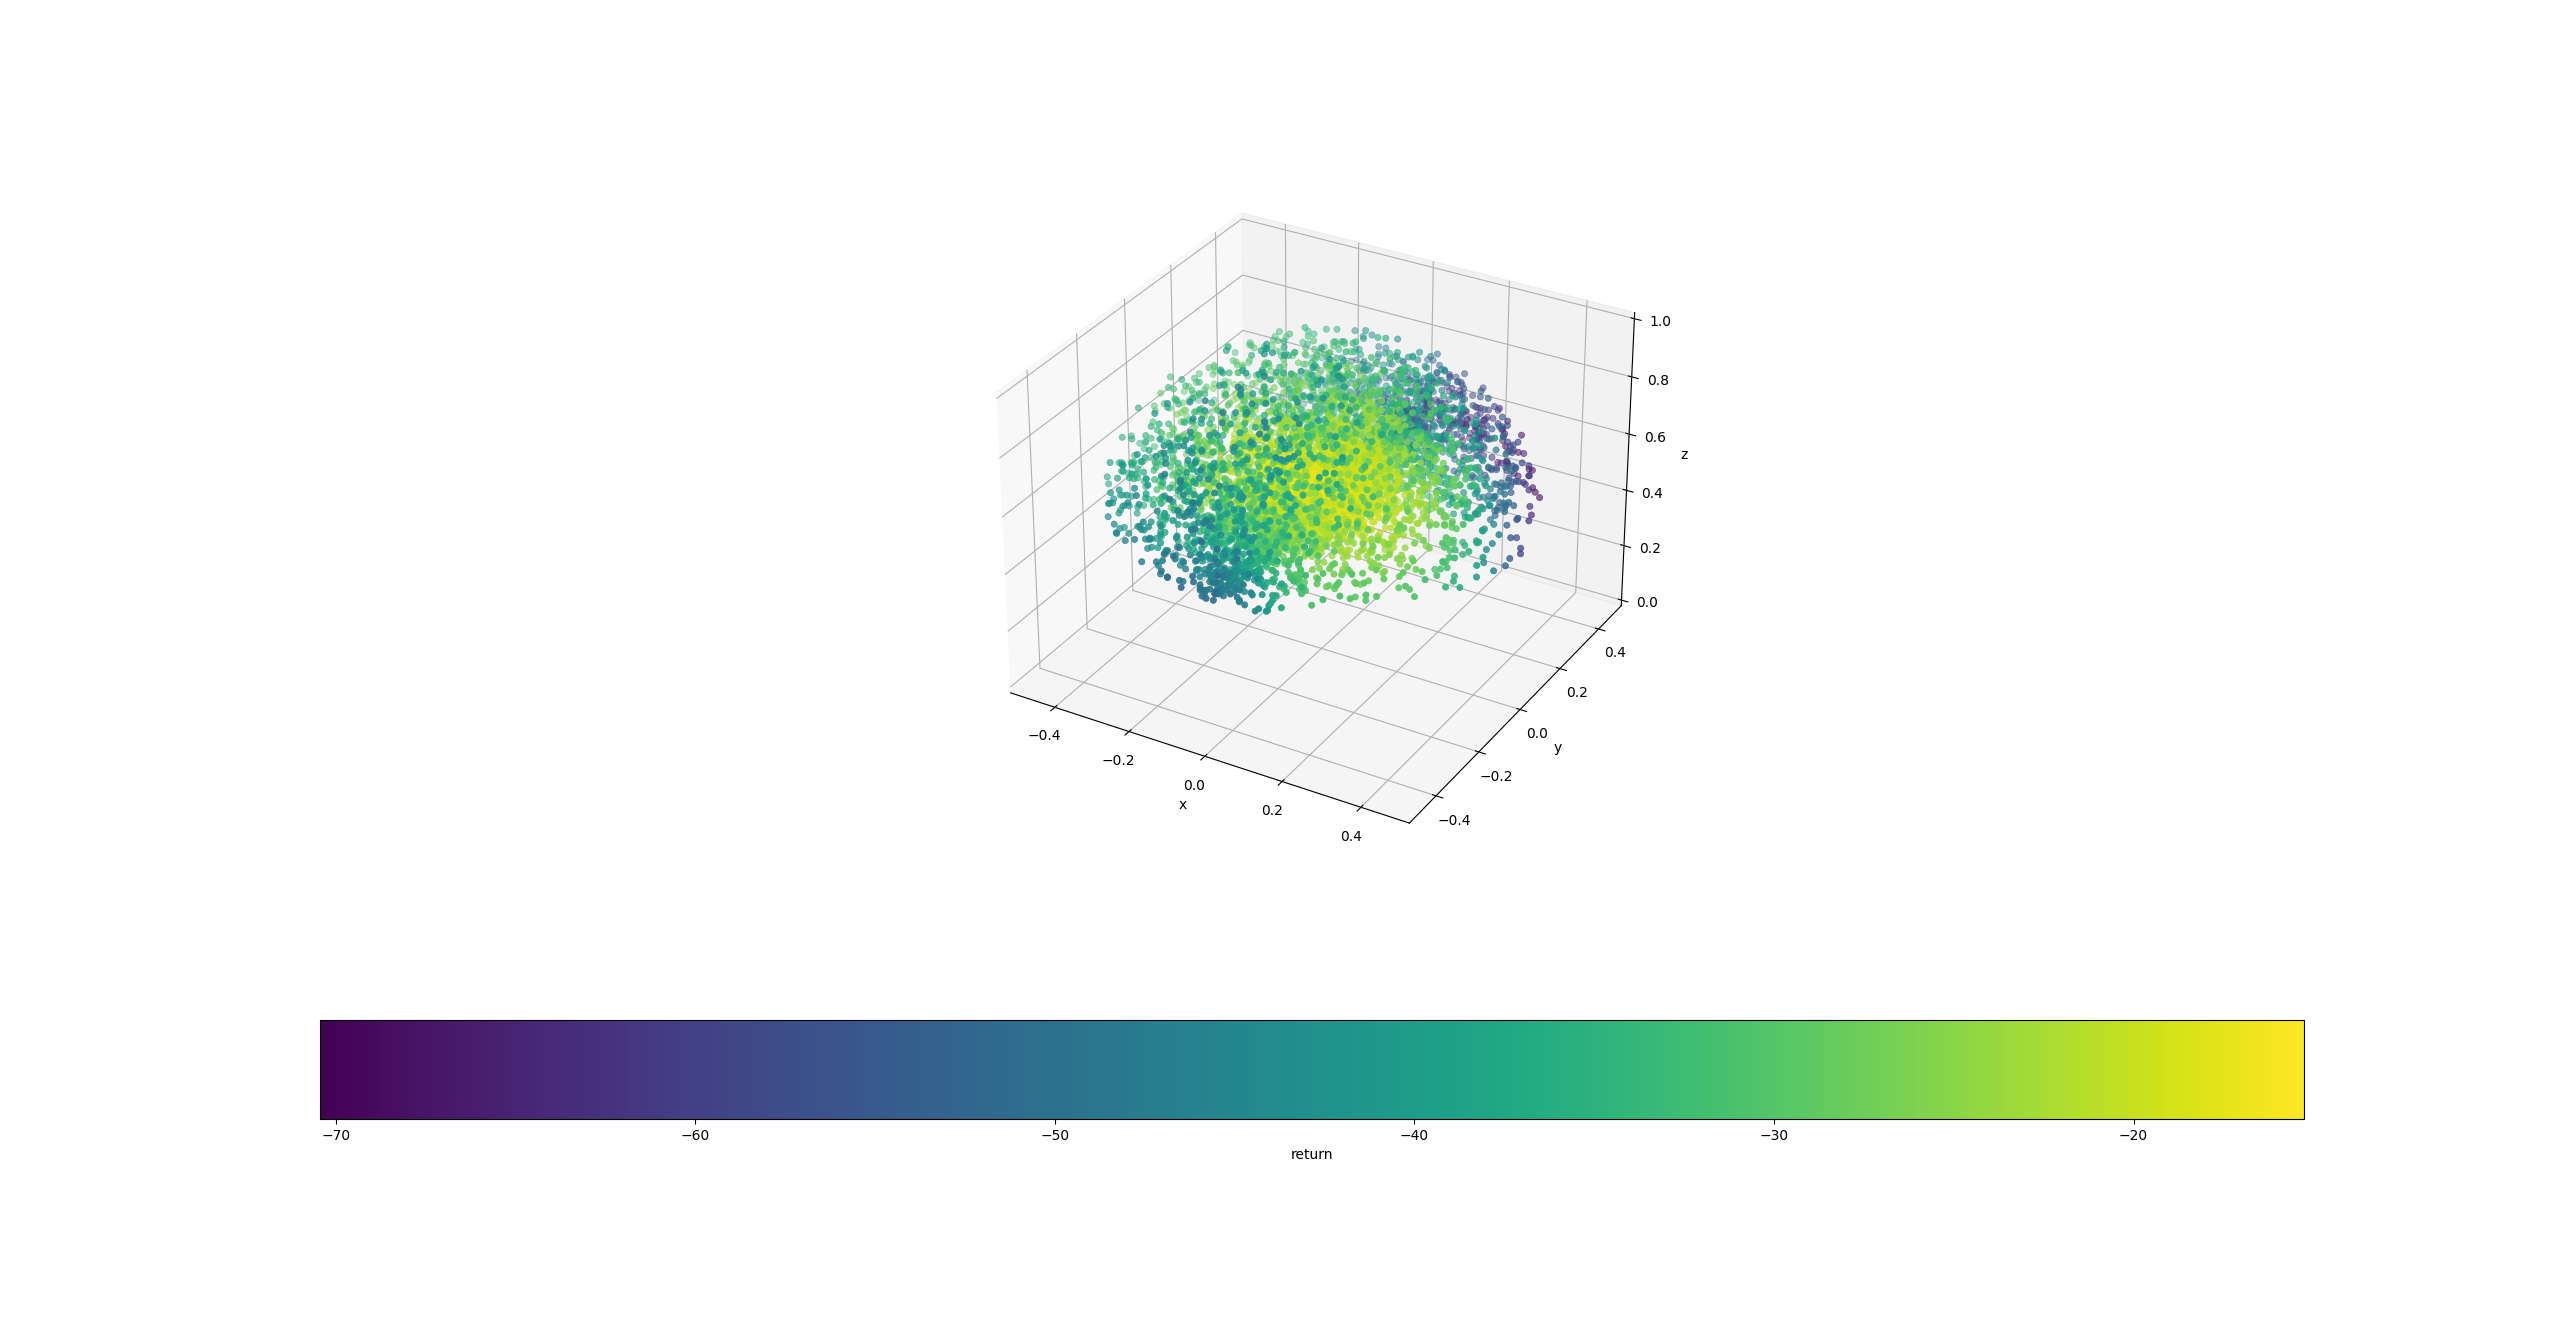
\includegraphics[width=\linewidth]{figures/potentialplot2.png}
	\caption{Expected Return of SAC policy with LCL ($\delta = 0.4$) for $7500$ random goals inside the 
	goal ball with a radius of $0.5m$}
	\label{fig:pot2}
\end{figure}

\begin{figure}
	\centering
	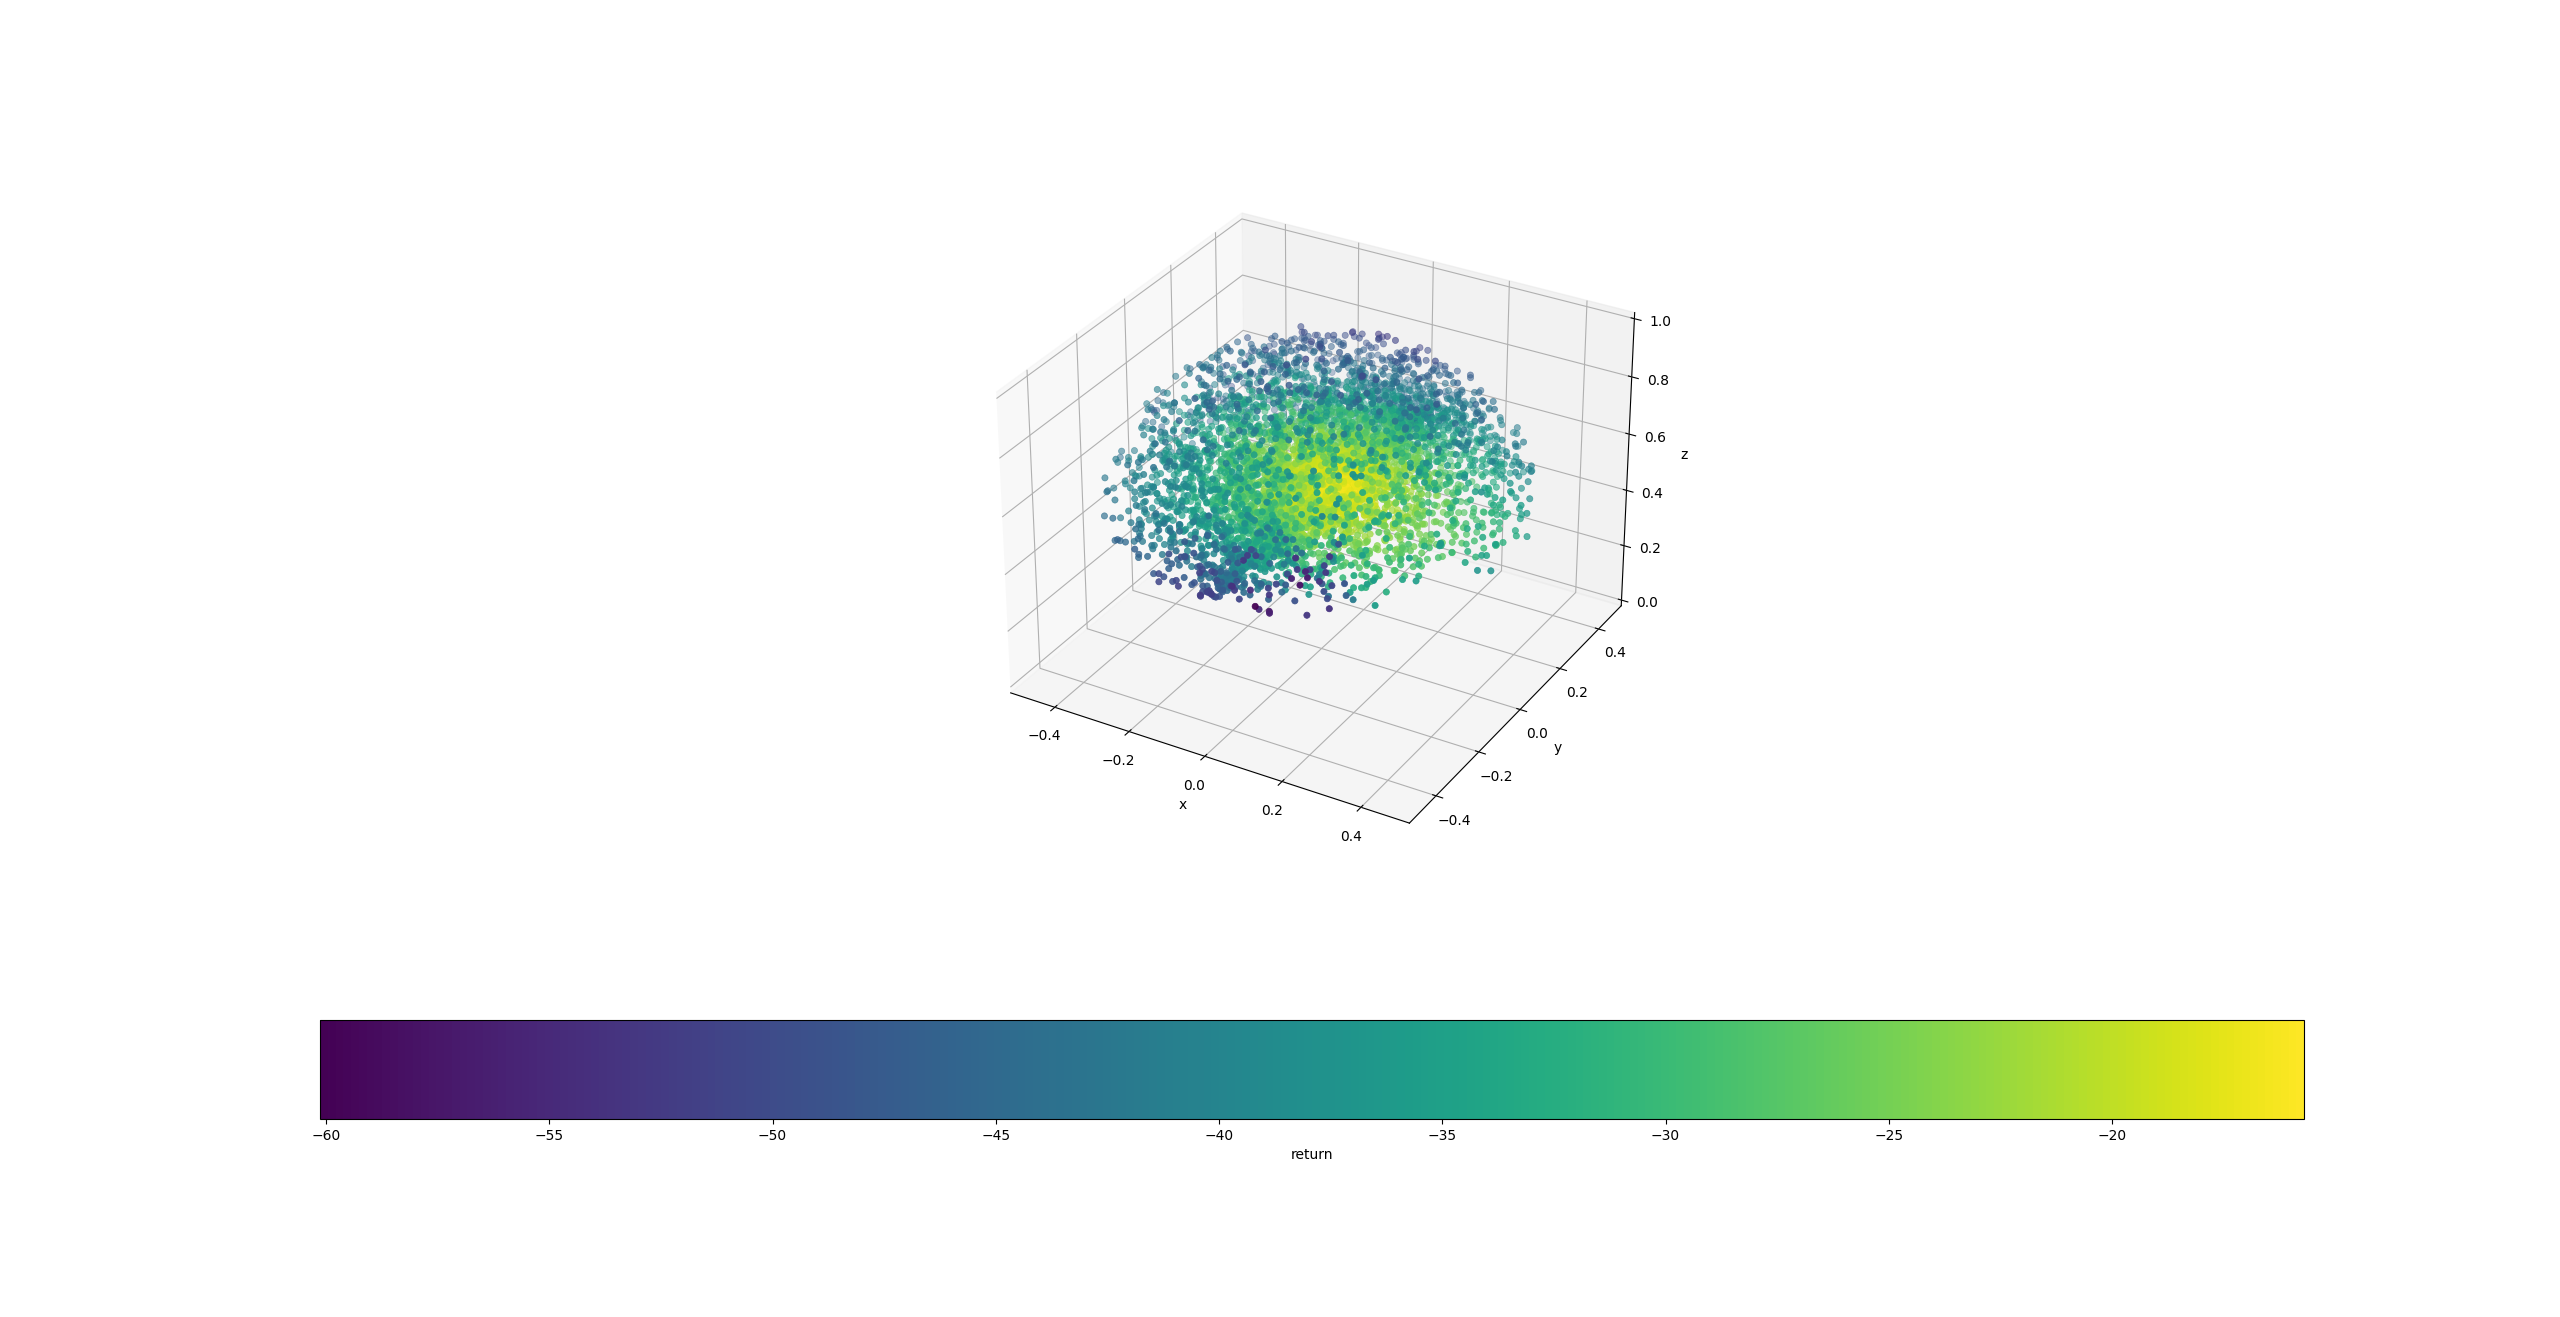
\includegraphics[width=\linewidth]{figures/potentialplot3.png}
	\caption{Expected Return of SAC policy with LCL ($\delta = 0.2$) for $7500$ random goals inside the 
	goal ball with a radius of $0.5m$}
	\label{fig:pot3}
\end{figure}

\begin{figure}
	\centering
	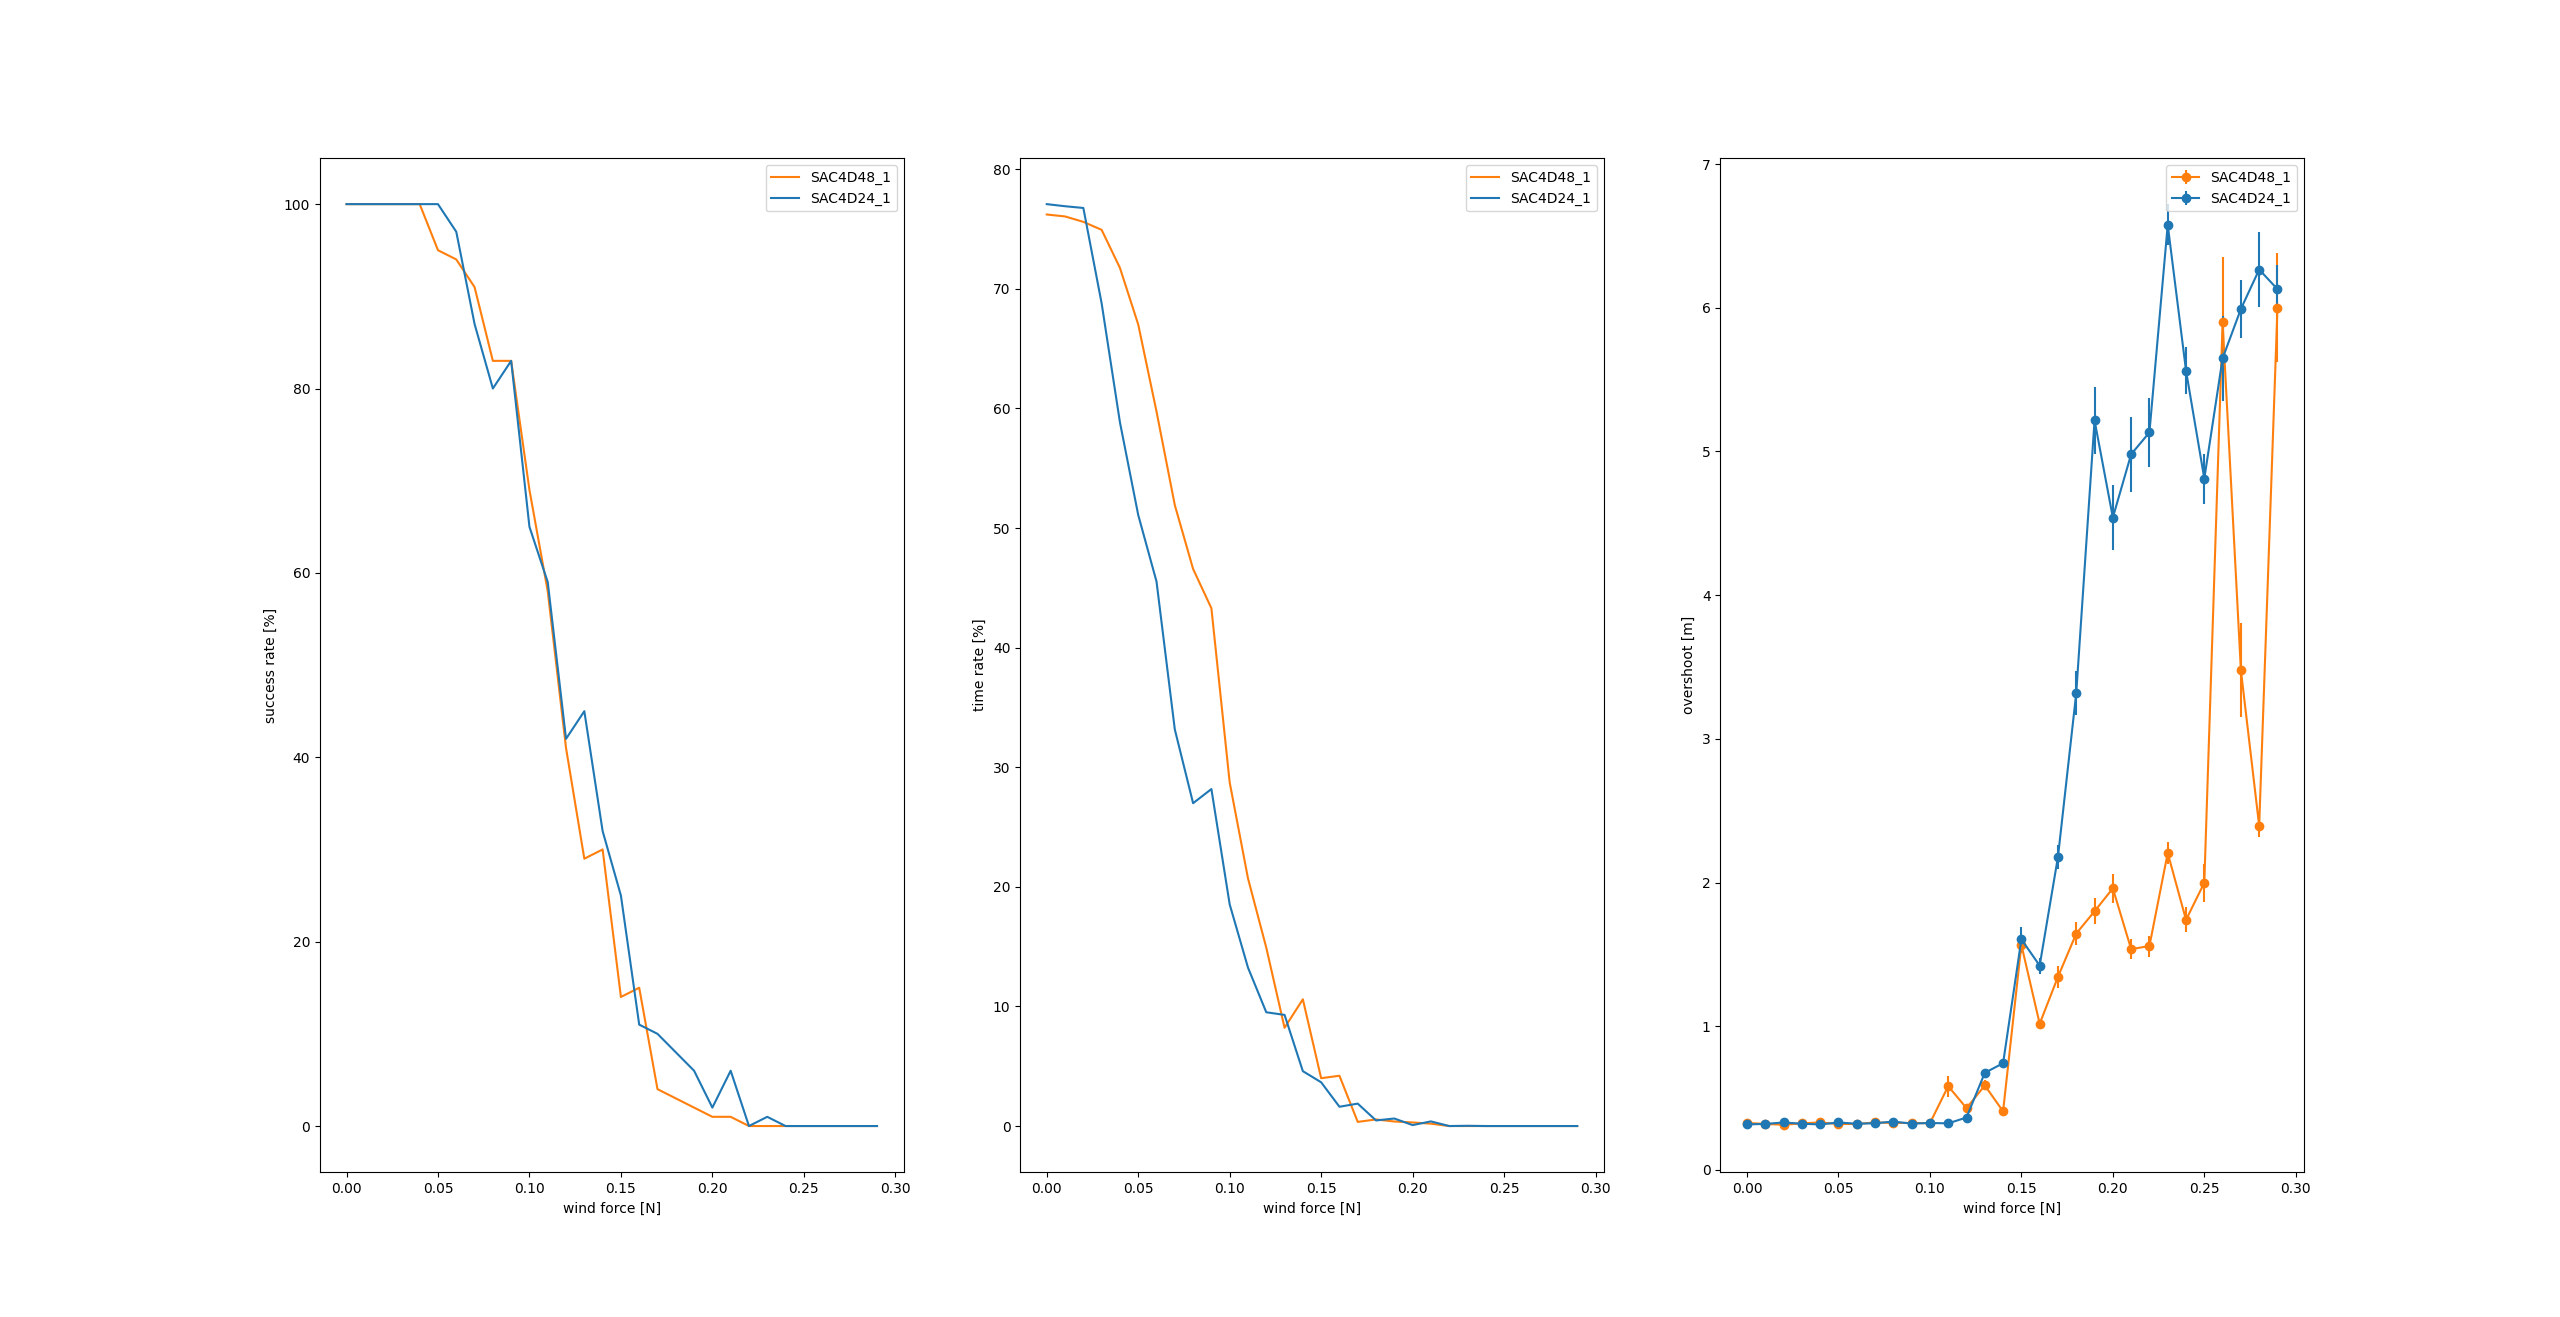
\includegraphics[width=\linewidth]{figures/windsuc.png}
	\caption{Success rate, time rate and overshoot $[m]$ with the associated standard error
	of SAC4D48 (orange) and SAC4D24 (blue) in a wind field of different strengths between $0N$ and $0.3N$}
	\label{fig:succ}
\end{figure}


\chapter*{List of Symbols}
\addcontentsline{toc}{chapter}{List of Symbols}

\begin{description}
	\item $\Theta$ \dotfill Roll Euler Angle
	\item $\phi$  \dotfill Pitch Euler Angle
	\item $\psi$ \dotfill Yaw Euler Angle
	\item $M_i \qquad i \in [1,4]$ \dotfill Motor of a Quadrocopter
	\item $\tilde{f}$ \dotfill Upward Thrust of a UAV
	\item $\omega_i \qquad i \in [1,4]$ \dotfill  Rotational speed of a propeller of a Quadrocopter
	\item $\omega_i^* \qquad i \in [1,4]$ \dotfill Changed Rotational speed 
	\item $b$ \dotfill Quadrocopter constant
	\item $u_{\Theta}, u_{\phi}, u_{\psi}$ \dotfill Rotational movement
	\item $p_{3D}$ \dotfill Pose in 3D space
	\item $x_p, y_p, z_p$ \dotfill Coordinates in 3D space
	\item $F$ \dotfill Upward Thrust Force
	\item $G$ \dotfill Gravitational Force
	\\
	\item $g$ \dotfill Mission Goal
	\item $a$ \dotfill Attitude
	\item $a^*$ \dotfill Estimated Attitude
	\item $e_a$ \dotfill Attitude Error
	\item $S$ \dotfill Set of Motor Signals
	\item $p$ \dotfill Estimated Pose
	\item $p_{3D}^*$ \dotfill Estimated 3D Pose
	\item $(K_p, K_i, K_d), (K, T_n, T_v)$  \dotfill Tuple of PID control gains
	\item $u(t)$ \dotfill Control Signal
	\item $e(t)$ \dotfill Error Signal
	\item $\tilde{T}$ \dotfill Sampling Time Period
	\item $f'$ \dotfill Throttle Coefficient
	\item $m_{i,\Theta} , m_{i, \phi}, m_{i, \psi}$ \dotfill Mixer Values of the Motors
	\item $\Lambda$ \dotfill Set of Waypoints
	\item $\lambda_i \qquad i \in [0...n]$ \dotfill Waypoint
	\\
	\item $S$ \dotfill Set of states
	\item $A$ \dotfill Set of actions
	\item $R$ \dotfill Reward function
	\item $P$ \dotfill State Transition probability
	\item $p_0$ \dotfill Starting State Distribution
	\item $s_t$ \dotfill Observed State at timestep $t$
	\item $s_t^*$ \dotfill Real State at timestep $t$
	\item $a_t$ \dotfill Action at timestep $t$
	\item $r_t$ \dotfill Reward at timestep $t$
	\item $\pi$ \dotfill Policy
	\item $\pi^*$ \dotfill Optimal Policy
	\item $\tau$ \dotfill Trajectory
	\item $T$ \dotfill Amount of steps in a trajectory
	\item $\gamma$ \dotfill Discount factor
	\item $V^{\pi}(s)$ \dotfill Value Function under a policy
	\item $V^*(s)$ \dotfill Optimal Value Function
	\item $Q^{\pi} (s,a)$ \dotfill Q Function under a policy
	\item $Q^*(s,a)$ \dotfill Optimal Q Function
	\item $x_i$ \dotfill Input to a NN
	\item $w_i$ \dotfill Weight of edge in a NN
	\item $g()$ \dotfill Activation Function
	\item $\Theta$ \dotfill Policy Parameters
	\item $\phi$ \dotfill Value Function Parameters in PPO
	\item $L(s_t, a_t, \Theta_{old}, \Theta)$ \dotfill Policy Loss in PPO
	\item $g(\epsilon, A)$ \dotfill Surrogate Objective
	\item $\epsilon$ \dotfill Learning Rate
	\item $A$ \dotfill Advantage Function
	\item $\alpha$ \dotfill Trade-Off coefficient in SAC
	\item $H$ \dotfill Entropy
	\item $\mathcal{D}$ \dotfill Replay Buffer
	\item $L(\phi_i, \mathcal{D})$ \dotfill Loss Function in SAC
	\item $d$ \dotfill Done Value
	\item $y(r, s', d)$ \dotfill Target in SAC
	\item $\tilde{a}$ \dotfill Next Action sampled from the policy
	\item $\mathcal{B}$ \dotfill Batch of Transitions
	\item $\rho$ \dotfill Polyak averging hyperparameter
	\\
	\item $\overrightarrow{g}$ \dotfill Goal Vector
	\item $g_x, g_y, g_z$ \dotfill Goal Coordinates
	\item $p$ \dotfill Position Tupel
	\item $\overrightarrow{p_t}$ \dotfill Position Vector at time step $t$
	\item $\dot{p_i} \qquad i \in \{x,y,z\}$ \dotfill Linear Velocities
	\item $\dot{\Theta}, \dot{\phi}, \dot{\psi}$ \dotfill Angular Velocities
	\item $\sigma$ \dotfill Sensor Values
	\item $f_s$ \dotfill Simulation Frequency
	\item $\aleph$ \dotfill Number of physics steps within a step
	\item $\omega_w$ \dotfill Wind Force Bound
	\item $T$ \dotfill Episode length
	\item $R$ \dotfill Radius
	\item $\overrightarrow{W}$ \dotfill Wind Force Vector
	\item $\overrightarrow{p_0}$ \dotfill Starting State Vector
	\item $z_{min}$ \dotfill Minimum height of Coordinate Frame
	\item $\daleth$ \dotfill Observation Space
	\item $\daleth_t$ \dotfill Observation at time step $t$
	\item $v_i \qquad i \in [0,11]$ \dotfill Predefined Clipping Values
	\item $dist_t$ \dotfill Distance at time step $t$
	\item $t_s$ \dotfill Simulation time step
	\item $r_{opt}$ \dotfill Optimal Reward
	\item $f_c$ \dotfill Control Frequency
	\item $m$ \dotfill Mass of UAV
	\\
	\item $\xi$ \dotfill Set of parsed arguments to a script
	\item $\tilde{\lambda}$ \dotfill Set of environment arguments
	\item $\nu$ \dotfill Amount of parallel training environments
	\item $t_{total}$ \dotfill Training steps
	\item $\iota$ \dotfill Parsed load parameter
	\item $\zeta$ \dotfill Parsed curriculum parameter
	\item  $\epsilon_t$ \dotfill Training environment
	\item $\epsilon_e$ \dotfill Evaluation environment
	\item $\epsilon$ \dotfill Environment
	\item $R_{max}$ \dotfill Maximum radius in LCL
	\item $\delta$ \dotfill Radius Step Size parameter in LCL
	\item $\tilde{\rho}$ \dotfill Parsed gui parameter
	\item $t^*$ \dotfill Real time
	\item  $t_{sim}$ \dotfill Simulation time
	\item $\Sigma$ \dotfill Threshold of EvalWriter
	\item $\gimel$ \dotfill Evaluation episodes
	\item $\beth$ \dotfill Time Rate
	\item $\mu_r$ \dotfill Mean return
	\item $\sigma_r$ \dotfill Std return
\end{description}

\chapter*{List of Abbreviations}
\addcontentsline{toc}{chapter}{List of Abbreviations}

\begin{description}
	\item DOF \dotfill Degree of Freedom
	\item FC \dotfill Flight controller
	\item PID controller \dotfill Proportional-Integral-Differential controller
	\item RL \dotfill Reinforcement Learning
	\item NLP \dotfill Natural Language Processing
	\item ML \dotfill Machine Learning
	\item MDP \dotfill Markov Decision Process
	\item NN \dotfill Neural Network
	\item PPO \dotfill Proximal Policy Optimization
	\item SAC \dotfill Soft Actor-Critic
\end{description}


%%%%%%%%%%%%%%%%%%%%%%%%%%%%%%%%%%%%%%%%%%%%%%%%%%%%%%%%%%%%%%%%%%%%%%%%%%%%%%%%
\bibliographystyle{mybabalpha-fl}
\bibliography{mybib}


\end{document}
